\documentclass{article}



\usepackage{arxiv}

\usepackage[utf8]{inputenc} % allow utf-8 input
\usepackage[T1]{fontenc}    % use 8-bit T1 fonts
\usepackage{hyperref}       % hyperlinks
\usepackage{url}            % simple URL typesetting
\usepackage{booktabs}       % professional-quality tables
\usepackage{amsfonts}       % blackboard math symbols
\usepackage{nicefrac}       % compact symbols for 1/2, etc.
\usepackage{microtype}      % microtypography
\usepackage{lipsum}		% Can be removed after putting your text content
\usepackage{graphicx}
\usepackage{subcaption}
\usepackage{siunitx} 	% for SI units
\usepackage{textcomp}
\usepackage{subfloat} % subfigures

%% small toc
\usepackage{setspace, tocloft}

%Modifies line spacing of the ToC
\setlength\cftparskip{-1.0pt}
\setlength\cftbeforesecskip{6.3pt}
\setlength\cftaftertoctitleskip{2pt}

%Makes dots after sections/subsections: Sections 1., 2.1., etc
\makeatletter
\renewcommand{\@seccntformat}[1]{\csname the#1\endcsname.\quad}
\makeatother

% new command \co that types CO_2. Definig commands with number (s.a. \co2) in latex is not really possible, so I chose \co
\newcommand{\co}{\text{CO\textsubscript{2} }}

%Makes the dots (above) appear in ToC
\let \savenumberline \numberline
\def \numberline#1{\savenumberline{#1.}}

%More space in tables
\def\arraystretch{1.5}


\setcounter{secnumdepth}{4}

\usepackage{titlesec}
\titleformat{\paragraph}
{\normalfont\normalsize\bfseries}{\theparagraph}{1em}{}
\titlespacing*{\paragraph}
{0pt}{3.25ex plus 1ex minus .2ex}{1.5ex plus .2ex}

\title{Milestone 3: Data Analysis Pipeline}

%\date{September 9, 1985}	% Here you can change the date presented in the paper title
%\date{} 					% Or removing it

\author{Bayrakceken, Kudret Aras\\
	03669629
	\And
	Belkhiria, Zied\\
	03653792
	\And
	Bueno Ulacia, Ion\\
	03726897
	\And
	Egger, Maximilian\\
	03735004
	\And
	Kern, Max-Emanuel\\
	03673151
	\And
	Krüger, Philipp \\
	03673587
	\And
	Martín Cruz, Daniel\\
	03727385
	\And
	Tarasewicz, Damian\\
	03734755
}

%%% Add PDF metadata to help others organize their library
%%% Once the PDF is generated, you can check the metadata with
%%% $ pdfinfo template.pdf
\hypersetup{
pdftitle={Group 1: Data Analysis Pipeline},
pdfsubject={stat.ML},
pdfauthor={Philipp~Krüger},
pdfkeywords={Datasets, COVID-19, Mobility Data, CO2 Data},
}

\begin{document}
\maketitle
\begin{abstract}
In this report we provide our data analysis pipeline. We explain our model in detail and explain which methods we used to obtain our results. Several machine learning methods are introduced, set up and utilized to predict the behavior of \co emissions for the eight main \co emitting countries.  We assume that for each \co emitting sector, we can introduce an indicator where recent, monthly data is readily available. Then, we extract the aforementioned behavior of \co emissions from these indicators for each sector and combine the sectors later. We show our main result and discuss its validity at the end of this report. Currently, our front-end displays the indicators for each sector, covid related data, greenhouse gas data and our current model pipeline. Finally, we explain our further steps regarding the COVID-19 correlations, the front-end and the video.
\end{abstract}


% keywords can be removed
%\keywords{Datasets \and COVID-19\and Mobility Data\and  CO2 Data}


%\setcounter{tocdepth}{1}
\tableofcontents

%Deliverable:
%Submit a document describing
%the data processing pipeline
%the set of candidate machine learning models and
%a short summary of your preliminary assessment of candidate ML models.
%
%A mock-up of a front-end to use and explain the model (design).
%A Python software, implementing a running data analysis pipeline using a simple
%(dummy) test set for testing and verification.

\newpage
\section{Introduction}

In this report, we want to introduce you to our model and discuss several aspects of it, especially its advantages and shortcomings. Eventually, we will see if our model is a valid approach. We researched a lot on data, as this is the most integral part of our project. Unfortunately, a lot of the data we found did not match our criteria of being very up-to-date, having at least a monthly resolution and being publicly accessible. We therefore came up with several ways to especially address the first two criteria.

In the end, we want to see if we can say that countries with higher case numbers of COVID-19 also have less \co emissions and how this is related to one another.
Thus, the two most important fields of data we used for our model are COVID-19 and \co data. We did not have any problems regarding COVID-19 data but had some issues with \co data. Emission data is not up-to-date and is only published as yearly emissions per country. However, the COVID-19 pandemic influences emissions on a shorter time-scale as of now. We thus had to predict and model emission data ourselves.  We first predicted yearly \co emissions in a business-as-usual scenario without COVID-19 and then estimated \co emissions with COVID-19. To do so, we used industry data and developed indicators from that. We even did this for each of the five major sectors of \co emitters of every country individually. Similar approaches can also be found in the literature, for example in~\cite{LeQuere2020}.

We will discuss our model, all our approaches and all techniques in more detail in the respective sections. We used several techniques to process our data, such as moving averages, SARIMA, polynomial regression and support vector machines. The front end will present the input data we used, the model pipeline we implemented and the final answer to the research question.


\section{Assumptions and Model Design}

%Introduction/goal
In this section, we want to briefly present the general assumptions and explain how we approached the issue of predicting real time $CO_2$ emissions, without having readily available emission data. The deviation from the usual emissions should then be used to find correlations with COVID-19 case numbers.%todo: Case numbers or deaths?

%Materials and Methods
The starting point of our analysis was the central question: How can we make as much use as possible from the EDGAR %todo source
dataset, which not only provides emission data per country, but also for the different sectors transport, international aviation/shipping, buildings, other industrial combustion, other sectors and power industry? 

The central hypothesis is as follows: \emph{The emissions of a sector is a function of indicators that measure the activity or demand of a specific economic branch.} We limit the overall analysis to eight important regions: USA, EU, Russia, Brazil, India, China, Japan and Canada. As some indicators are not reliably updated, we consider the first six months of 2020 as the time period of interest.

\subsection{Prediction of 2020 emissions with and without the COVID-19 crisis}

The goal was to find for each sector a method to extrapolate the general country trends from 2018, which is where the EDGAR data ends, to 2020. Here, we also tried to find out whether there exist a general seasonality for the emissions of a sector, and to find out which indicators work best to model the actual emission behavior. This is important as we don't want to confuse emission fluctuations in 2020 with general seasonal trends.

In order to predict the actual 2020 emissions, we need to find real time indicators for each sector such as activity, prices, etc. in order to correlate them with the emissions from the past. Afterwards, the indicator can be used as a tool to predict the actual sector emissions.

\subsection{Calculate the emission drop and correlate it with COVID-19 impact}

From the difference of the two values for 2020, we can estimate a total drop or increase in emissions per country. This can then be correlated with COVID-19 cases. Either we directly look at the correlation to see the general impact. Or we compare the drop or increase with the individual climate goal of the country. Doing the latter, we can estimate the degree that the crisis helped reaching the goal or not.
%Results

\subsection{Discussion and external factors}

In summary, the strength of this approach lies in the validity of the indicators.
%Discussion
External Influences, such as precipitation and other seasonal factors that impact the actual $CO_2$ concentration can be neglected. This is both a strength and a weakness of this approach, as we could not use real time $CO_2$ concentration data.

%Conclusion Outlook








%%%%%%%%%%%%%%%%%%%%%%%

\section{Data Processing Pipeline}

\subsection{Predicting CO\textsubscript{2} Emissions 2020}
\subsubsection{Motivation}
One of the major problems was to find emission data. Our EDGAR dataset ends in 2018. The goal of this part is to predict the emissions for the two next years 2019 and 2020 in the case that the COVID crisis didn't occur. The first idea was to find any relationship between the countries \co emissions and the different activities sector such as industry, mobility, international aviation etc.
The problem we encountered was that these data were not temporally overlapping. As mentioned before, our EDGAR emissions dataset ends in 2018 and the samples are yearly. Furthermore, our mobility and aviation data is daily and starting from January 2020. No relationship can be found if the data are not temporally crossing. The second idea was to predict these emissions for 2019 and 2020 from its evolution since 1970 .
\subsubsection{Predicted Country CO\textsubscript{2} Emissions without Considering COVID-19}
\paragraph*{Polynomial regression}
In order to predict the emissions for each country for the two next years starting from 2018 we need a model that describes the \co emissions evolution. A model based on regression learning is used. The first two questions arising are  which model to use and what the parameters of such a model should be.
Choosing between a linear and a polynomial model is evident. The evolution of \co is for many countries is too complex and a linear model does not offer enough precision to describe such curves.
The easiest curve to learn has is Bangladesh, shwowing an approximately exponential shape, which can be easily expressed with a polynomial. But there are complexer shapes where the emissions increase is not stable.
\begin{figure}[h!]
	\centering
	\subfloat[Bangladesh]{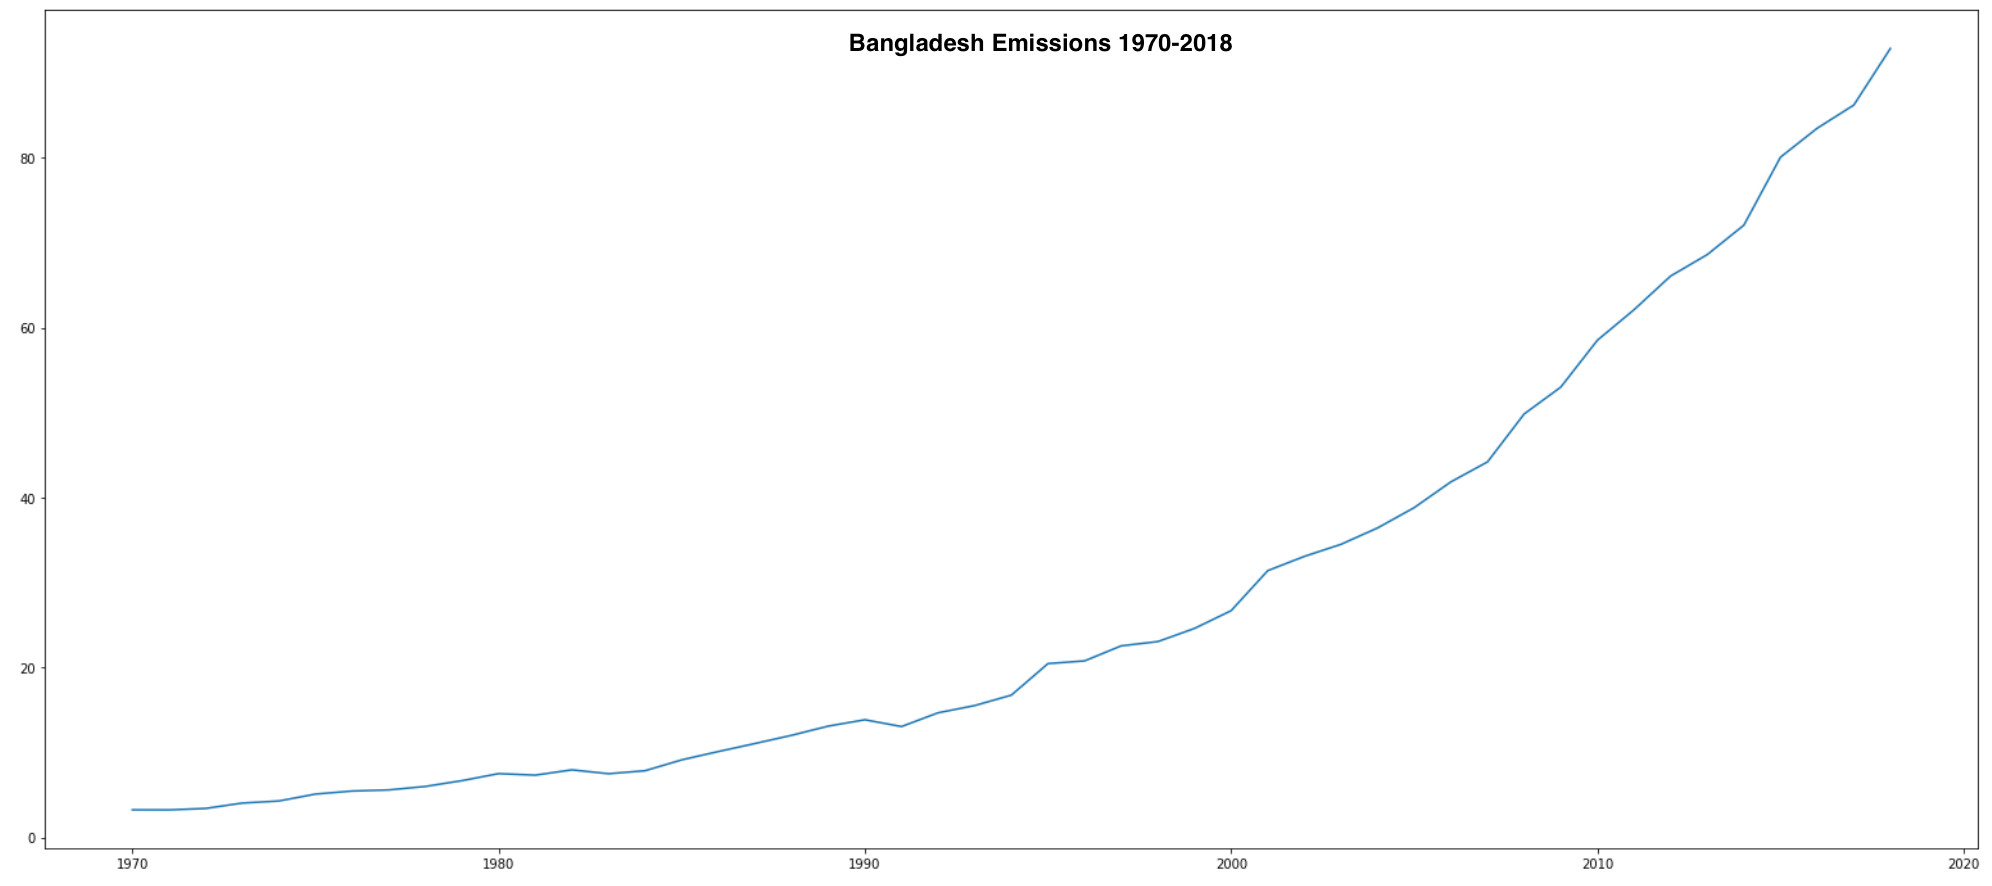
\includegraphics[width=0.5\linewidth]{ziedPNGS/Bangladesh}}
	\subfloat[Ireland]{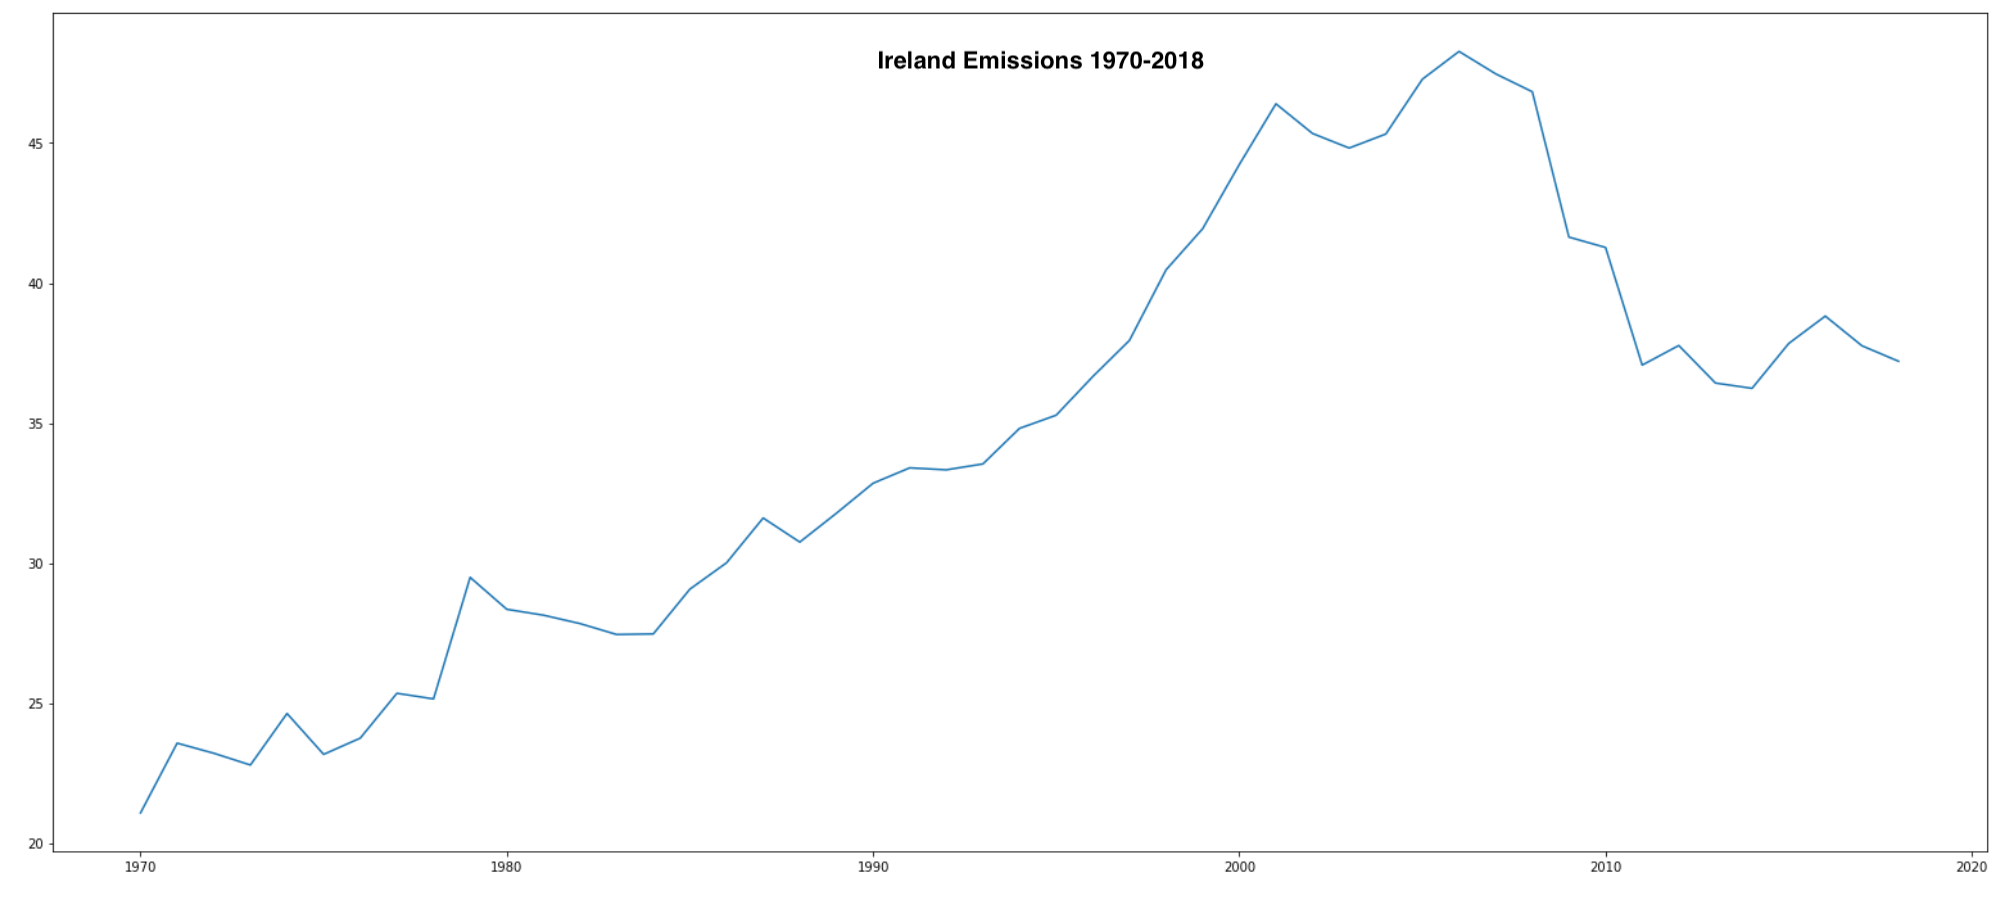
\includegraphics[width=0.5\linewidth]{ziedPNGS/Ireland}}
	\caption{Example of a stable and unstable emissions evolution.}
	\label{fig:Emissions}
\end{figure}
\newline
For choosing the size $k$ of a polynomial $\sum_{n=1}^{k}{a_n*x^n}$, fifteen models of size $k=[1,\dots,15]$ were trained and the results were compared to the real data using the root-mean-sqaure (RMS) in \autoref{fig:RMS}.
\begin{figure}[h!]
	\centering
	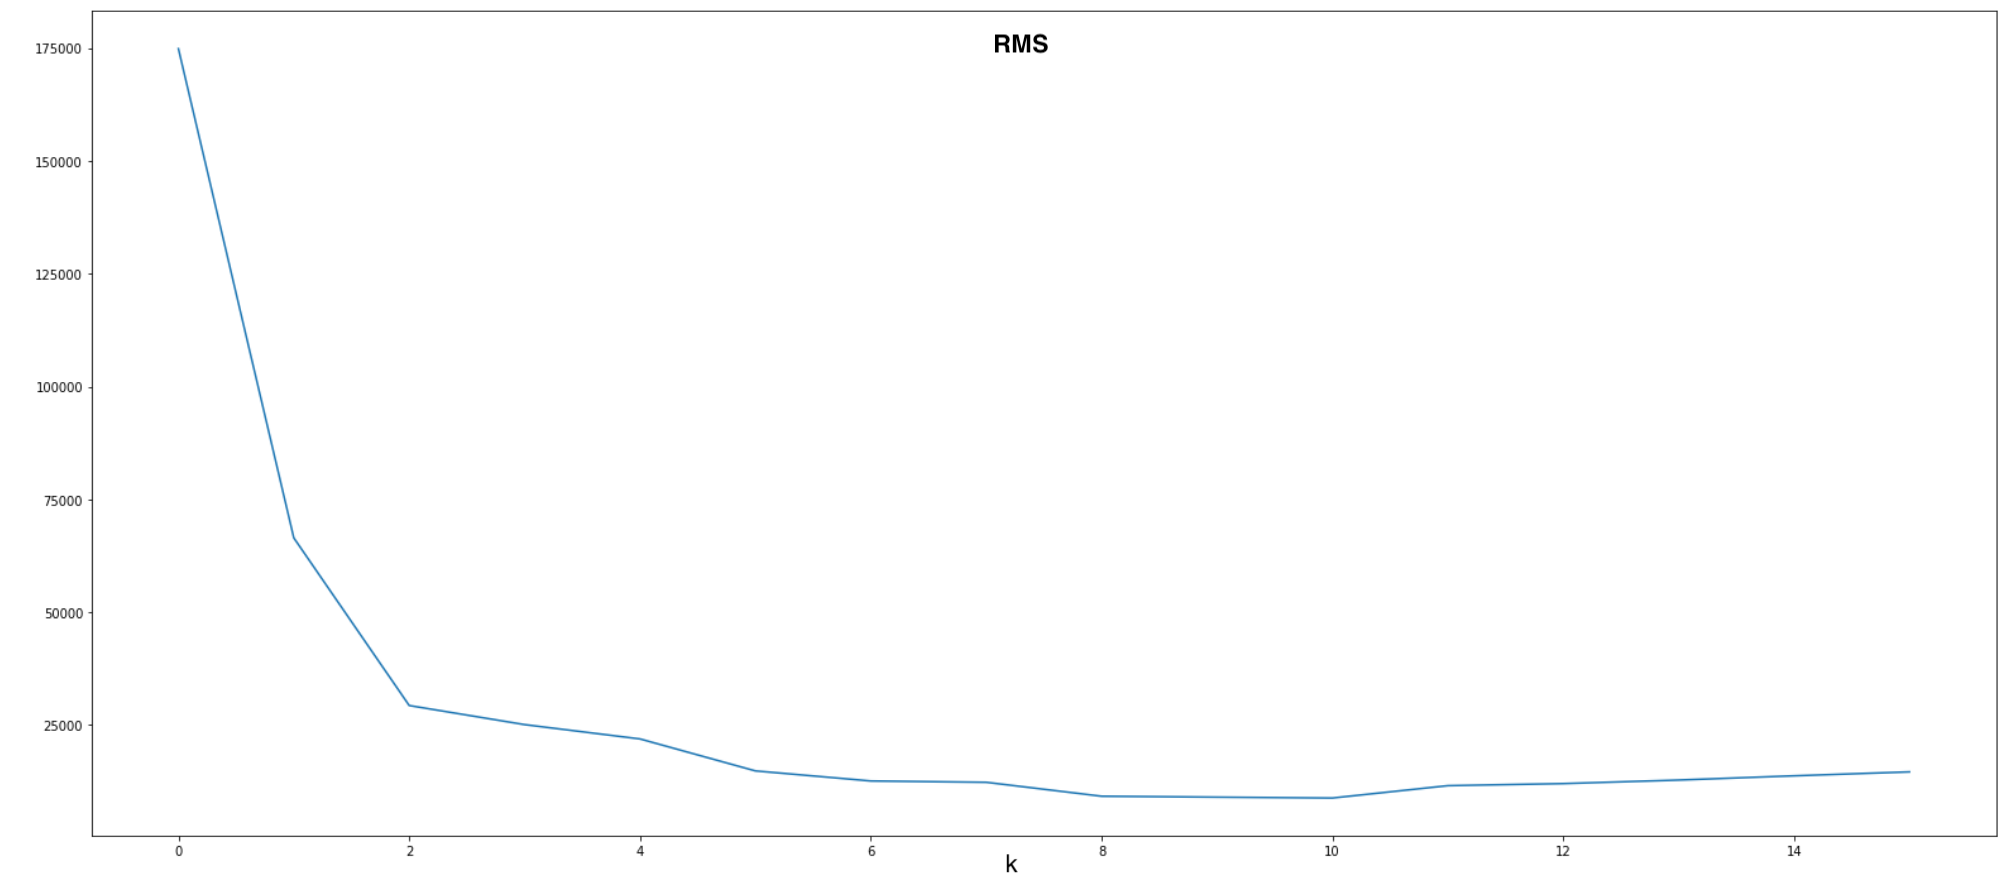
\includegraphics[width=0.7\linewidth]{ziedPNGS/RMS}
	\caption{$k=9$ delivers the smallest error.}
	\label{fig:RMS}
\end{figure}

\paragraph*{Polynomial regression's limitations}
After training a regression model for each country, the polynomials showed some plausible predictions but also many predictions where the curve has a steep drop for 2019 and 2020 \autoref{fig:firstPrediction}. The next step is to manage finding a plausible prediction for each of the eight important regions mentioned before.

\begin{figure}[h!]
	\centering
	\subfloat[Africa]{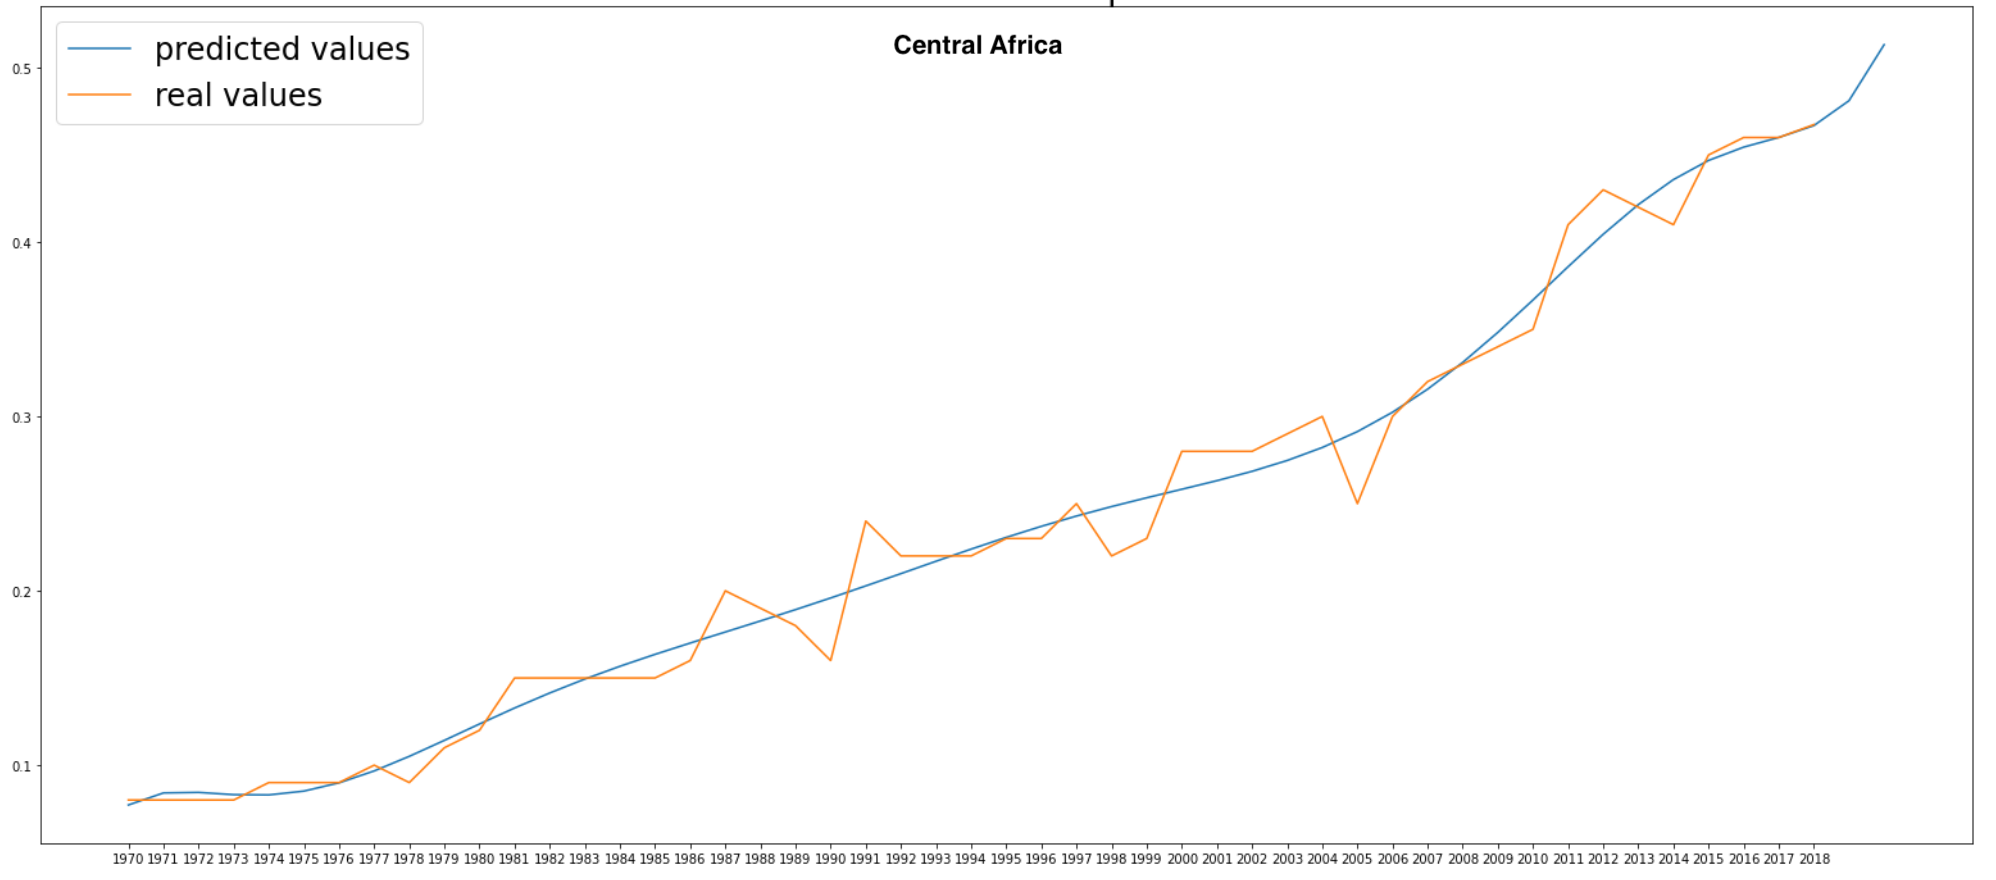
\includegraphics[width=0.5\linewidth]{ziedPNGS/Africa}}
	\subfloat[Chad]{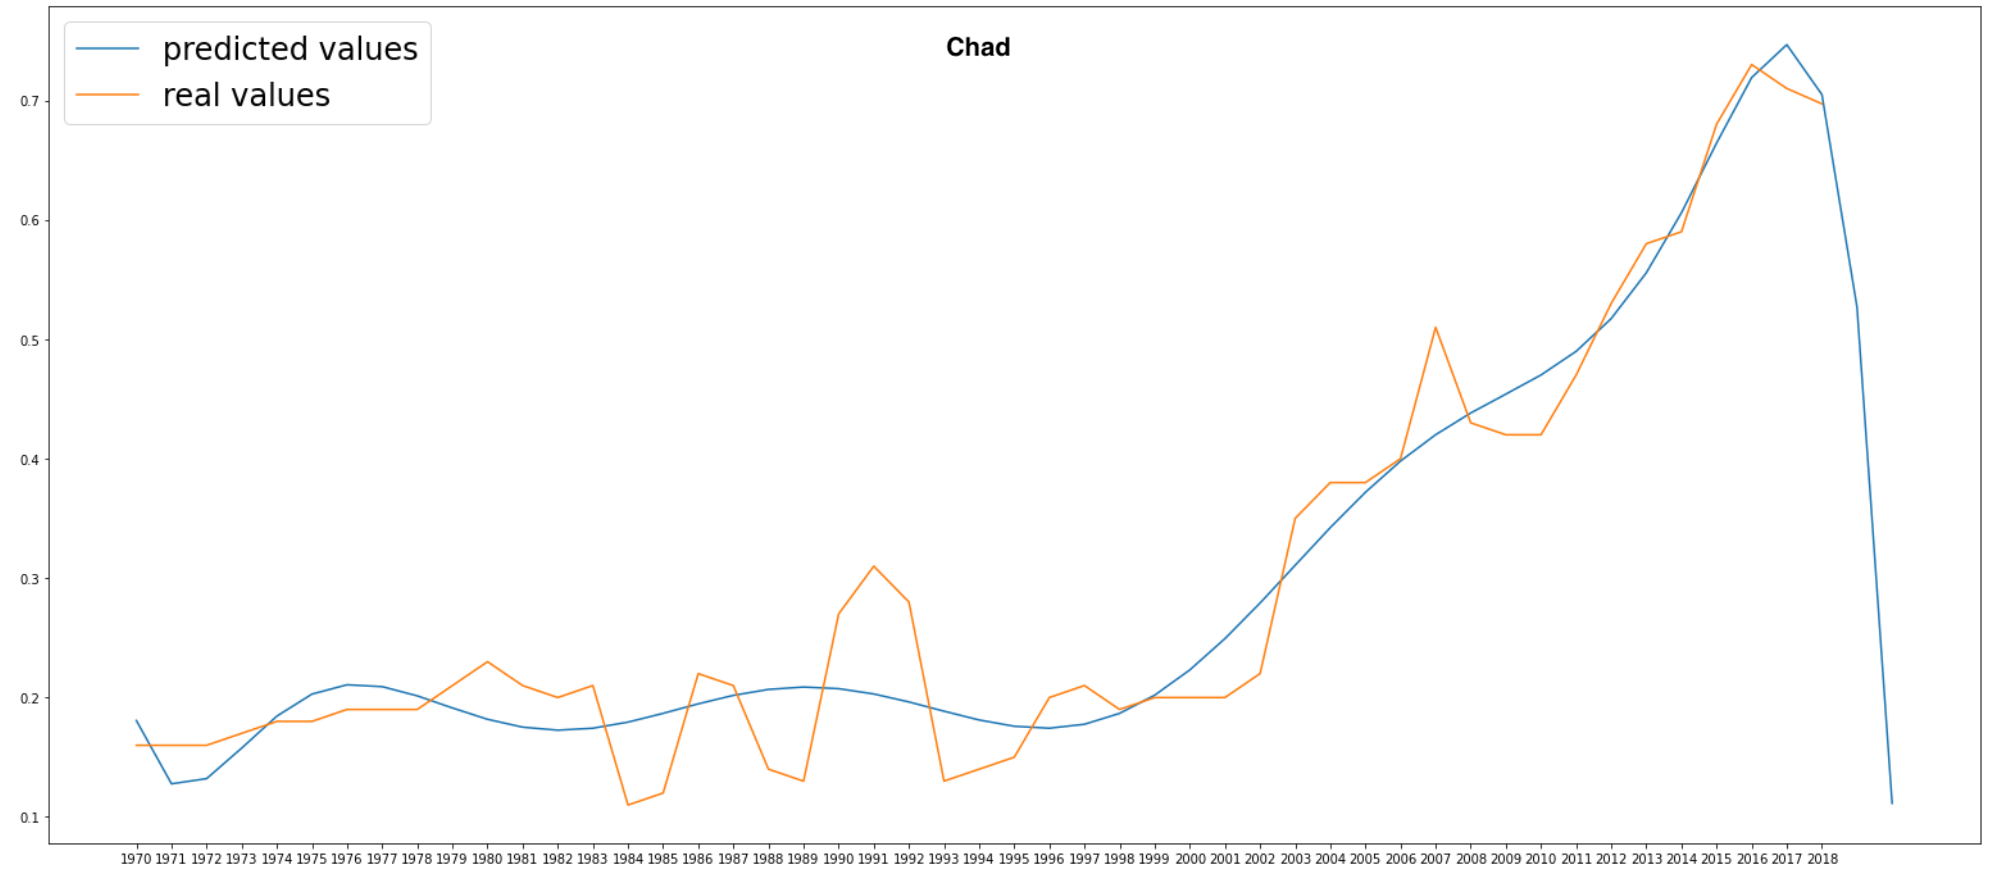
\includegraphics[width=0.5\linewidth]{ziedPNGS/Chad}}
	\caption{Example of a plausible and a wrong prediction}
	\label{fig:firstPrediction}
\end{figure}

\paragraph*{Correlation's predictions}
Looking closer to the EDGAR dataset, we can notice that some countries emissions are correlating. This make sense since the industry and a more resource-intensive way of life becomes more and more global. Using this assumption, one can take advantage of these correlations to correct the wrong predictions from our models.
Using the first prediction, we manually select the best results and look for countries with correlating emissions.
The first step is to choose the best predictions from our results. In our case we have 21 plausibly predicted values for 2019 and 2020. Having this list of countries we calculate the correlation of the real data from 1970 to 2018 of these 21 countries with every other country and filter out the correlations included in the interval $[-0.9,...,0.9]$.
Now we have a list of countries which emissions in 2019 and 2020 can be predicted from the first predictions.
For each correlation, we train a linear model using the real data from 1970 until 2018 and predict the emissions of 2019 and 2020 using the appropriate model and the predicted data from 1970 to 2020.
\begin{center}
\begin{table}[h!]%todo: Pie chart?, Values add up to 109 \% sadly
	\centering
	\begin{tabular}{ll}
		\hline
		 Country's emissions to predict& Already predicted countries emission\\
		\hline
		\hline
		 Bahrain   & Australia   \\
  		 Brazil &   Australia  \\
 		 Canada & Australia \\
 		 Dominica & Australia, Burkina Faso\\
  		 Iran & Australia, Burkina Faso, Egypt, Iceland, India, Indonesia \\
		 Iraq & Burkina Faso, India, Indonesia \\
 		 Ireland & Greece \\
		 Malta & Greece \\
 		 Haiti &  Burkina Faso, Egypt \\
 		 Singapore & Australia, Egypt, Indonesia, Malaysia, Morocco \\
 		 United Kingdom & Burkina Faso, Egypt, India, Morroco, Phlippines, Turkey, United Arab Emirates \\
 		 United States& Netherlands \\
		\hline &\\
	\end{tabular}
	\caption{Some examples of dependencies for the second predictions.}%todo: source
	\label{tab:correlations}	
\end{table}	
\end{center}
Some examples of our results are shown in the \autoref{tab:correlations}. We can see that Brazil is only correlating with Australia. In this case we predict Brazil's emissions from Australia's emissions. For Iran we have more countries correlating: Australia, Burkina Faso, Egypt and other. In this case, we can generate more predictions. From these predictions we calculate the mean value, the maximum value and the minimum value to have a better approximation.
\begin{figure}[h!]
	\centering
	\subfloat[Brazil]{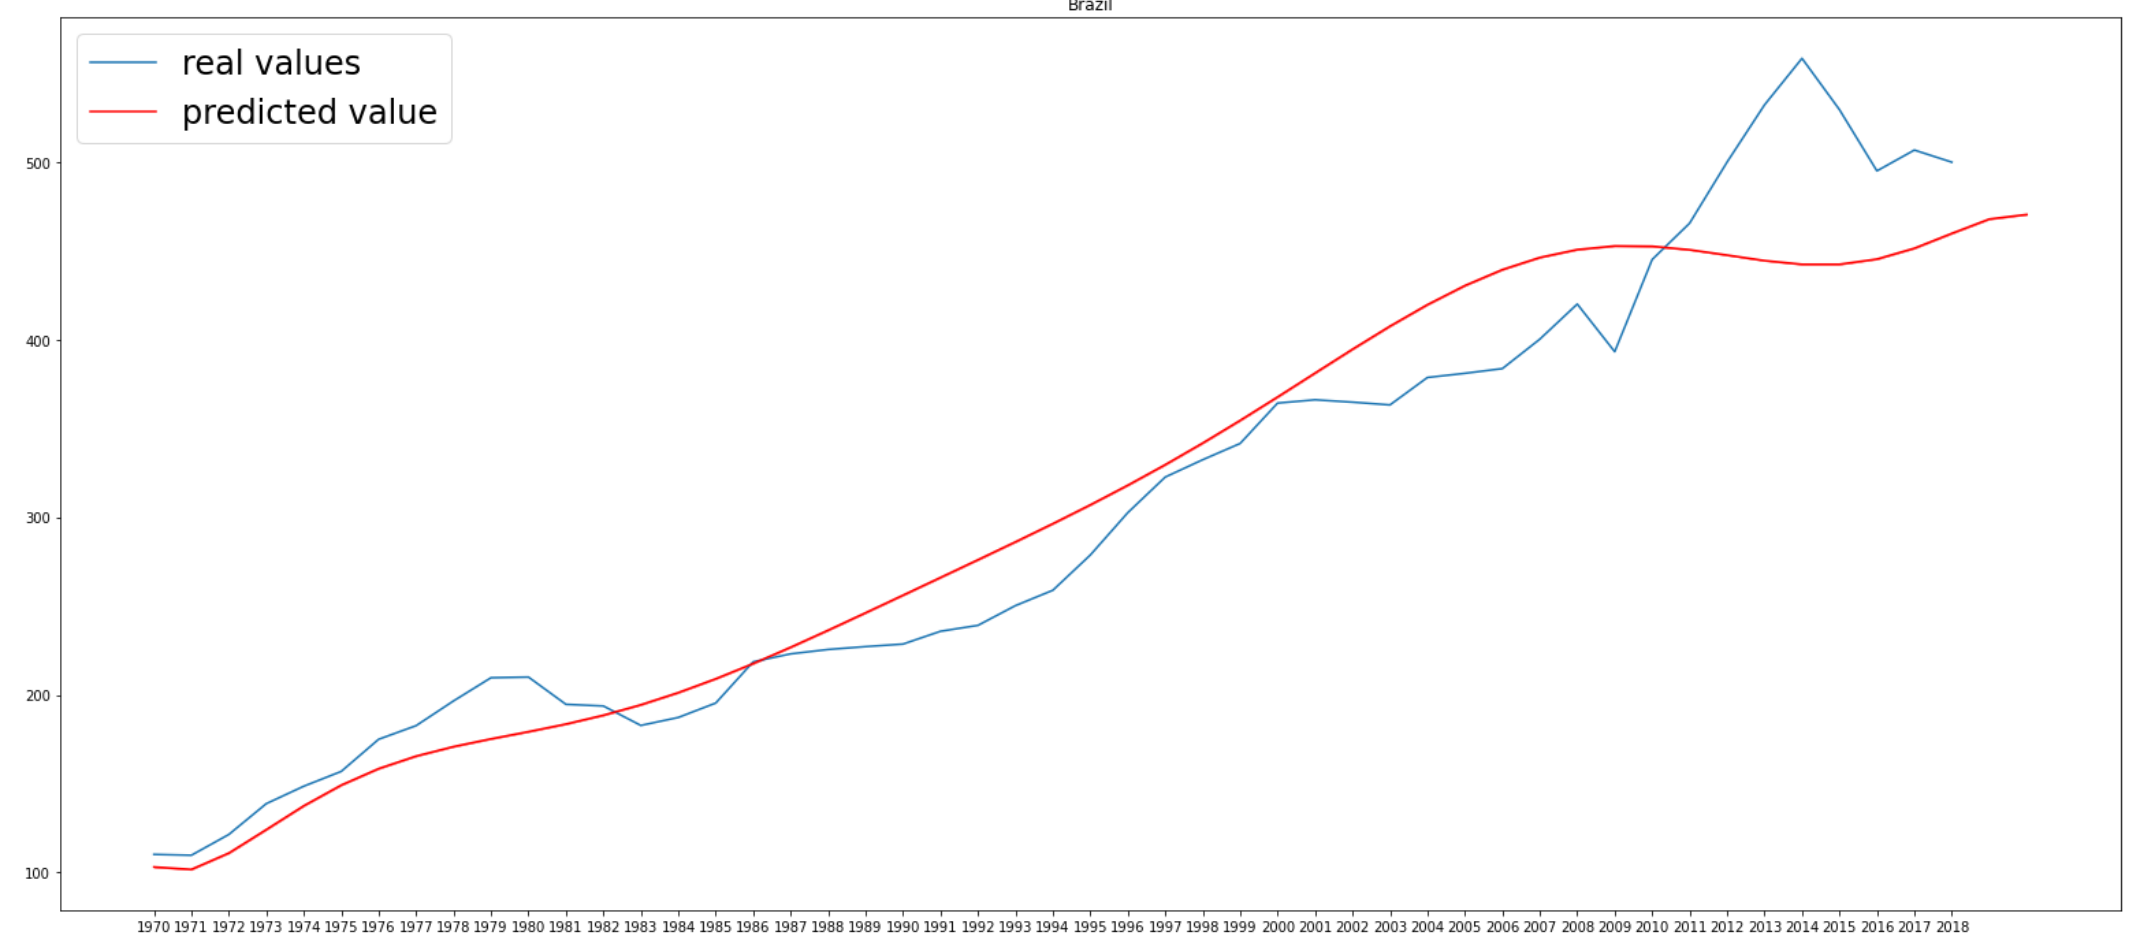
\includegraphics[width=0.5\linewidth]{ziedPNGS/Brazil}}
	\subfloat[Iran]{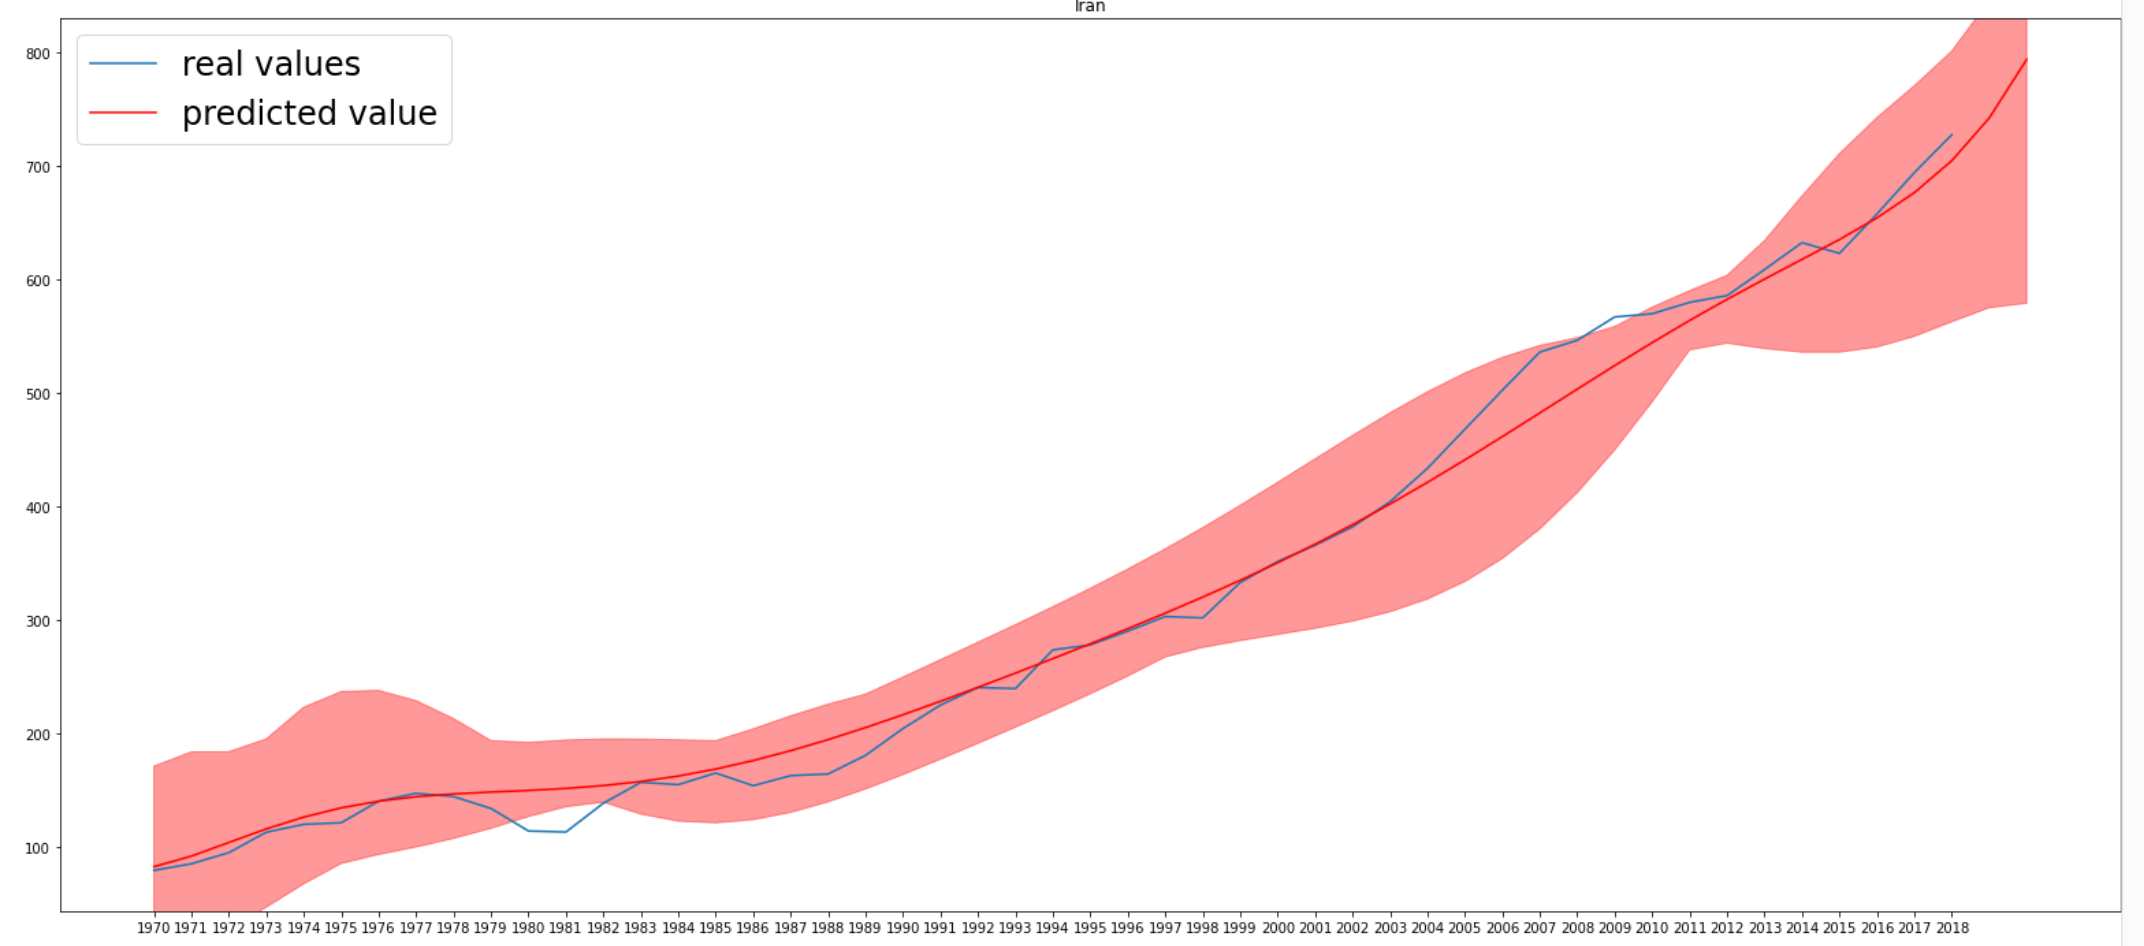
\includegraphics[width=0.5\linewidth]{ziedPNGS/Iran}}
	\caption{Brazil's emissions are predicted from Australia's emissions. Iran's emissions are predicted from the emissions of several countries.}
	\label{fig:resultsExample} % change label
\end{figure}

\subsubsection{Results and conclusion}
From the eight major countries we consider -- Canada, China, United States, Japan, Russia, Brazil, India and the EU -- India's predictions could be generated with the first prediction and the remaining countries were generated with the second predictions.
Only Russia's predictions are not available, because no correlation with any other country was found.

\begin{figure}[hbt!]
	\centering
	\subfloat[Brazil]{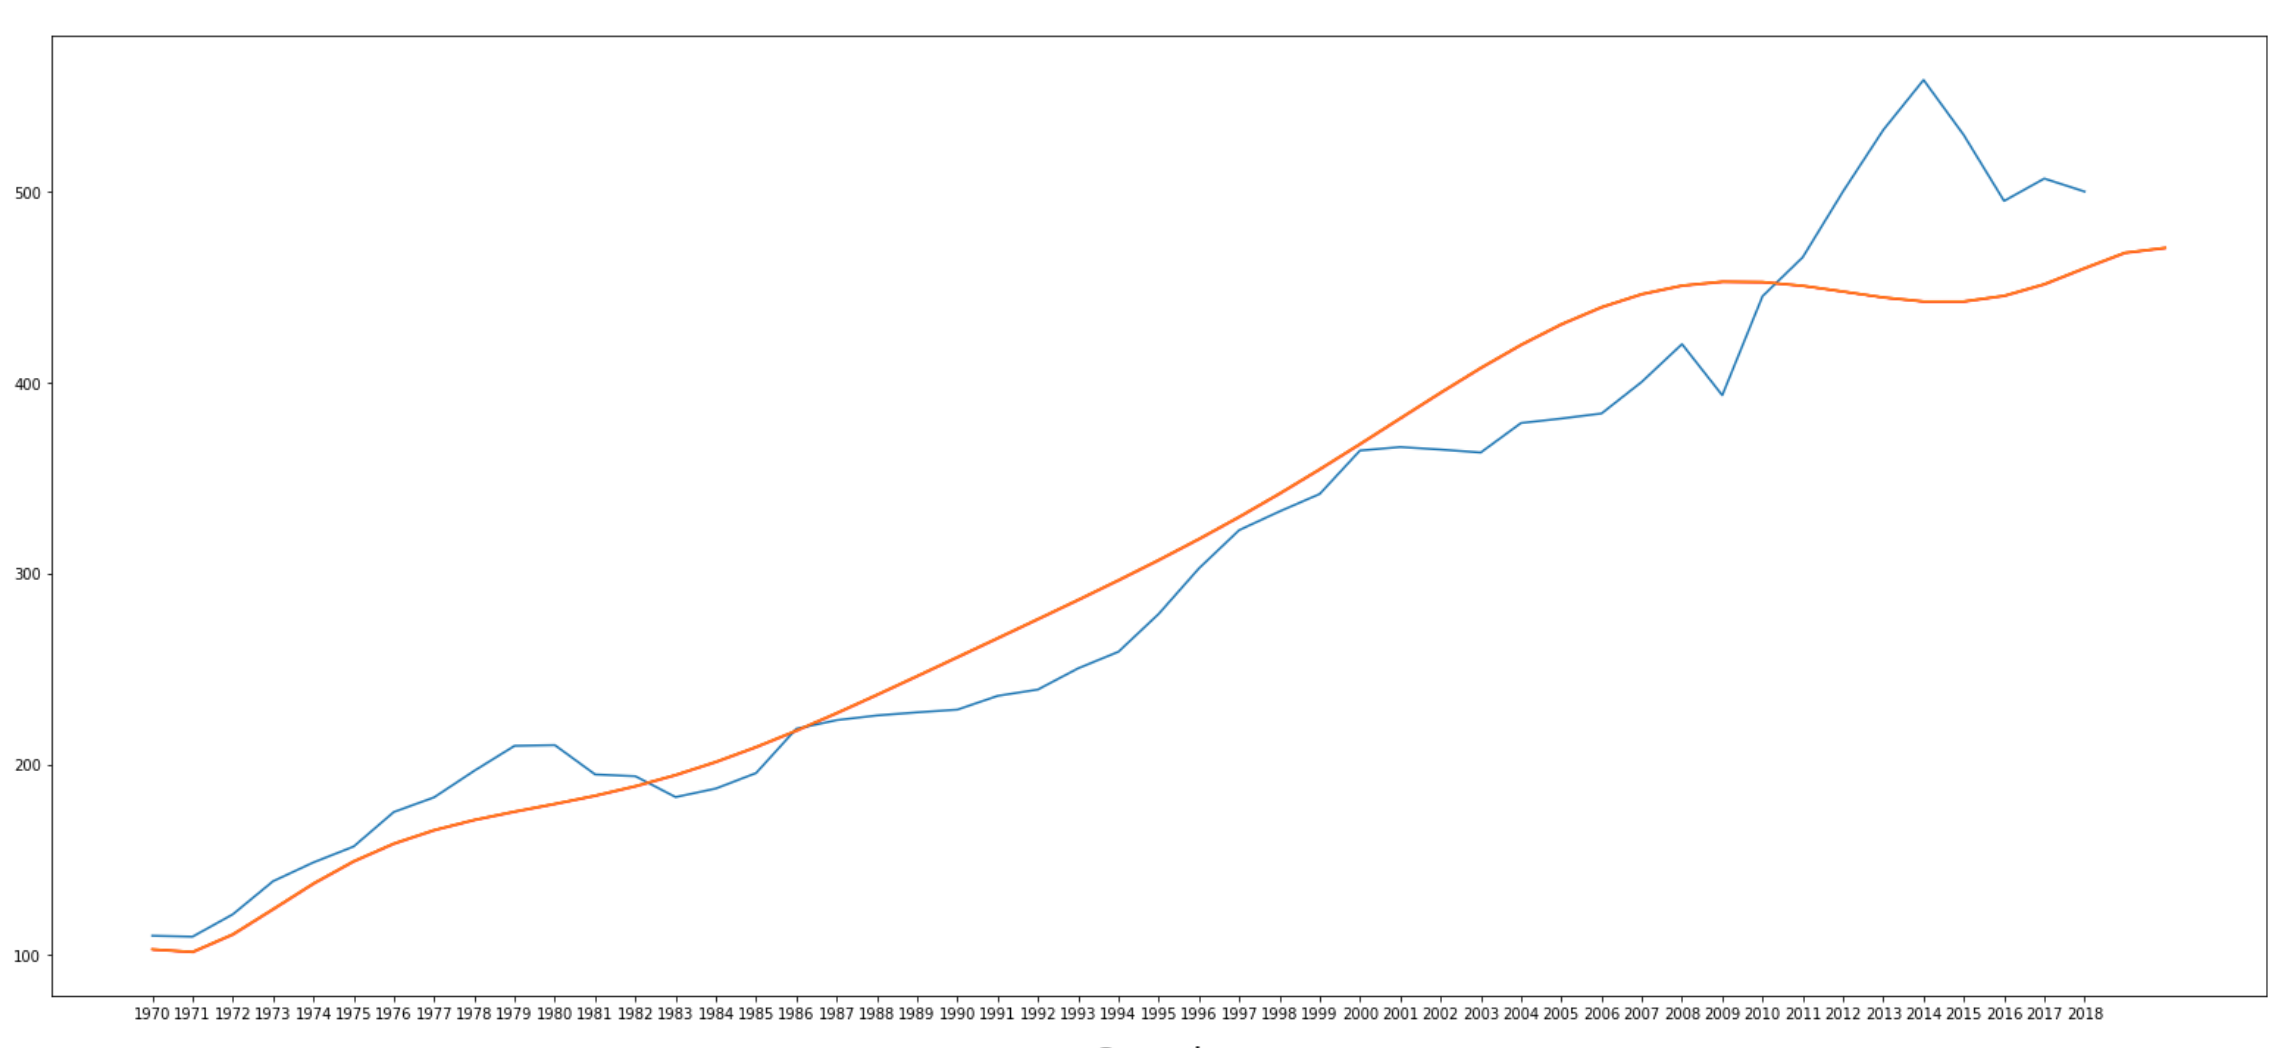
\includegraphics[width=0.5\linewidth]{ziedPNGS/br}}
	\subfloat[Canada]{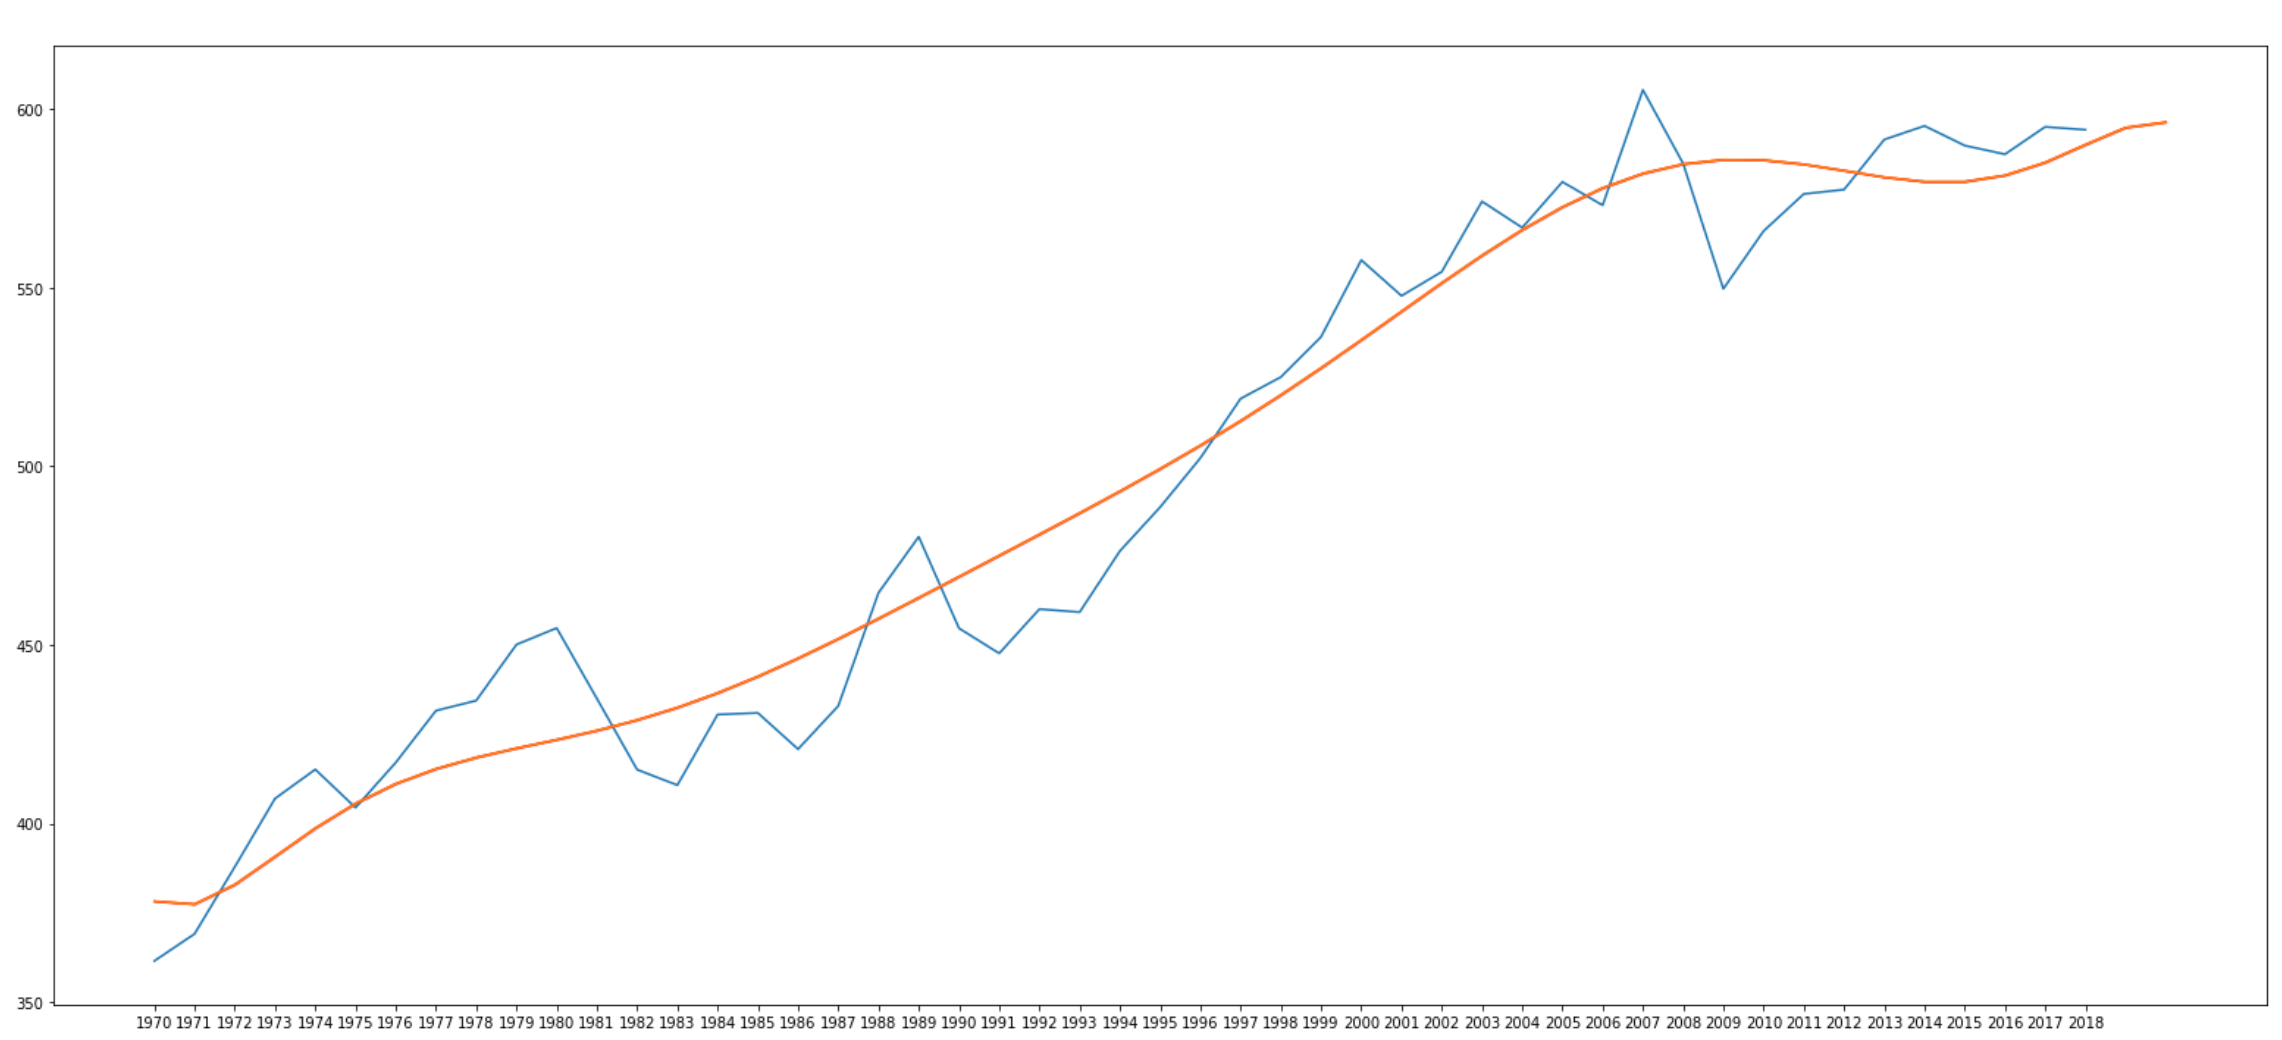
\includegraphics[width=0.5\linewidth]{ziedPNGS/2}}
	
	\subfloat[Japan]{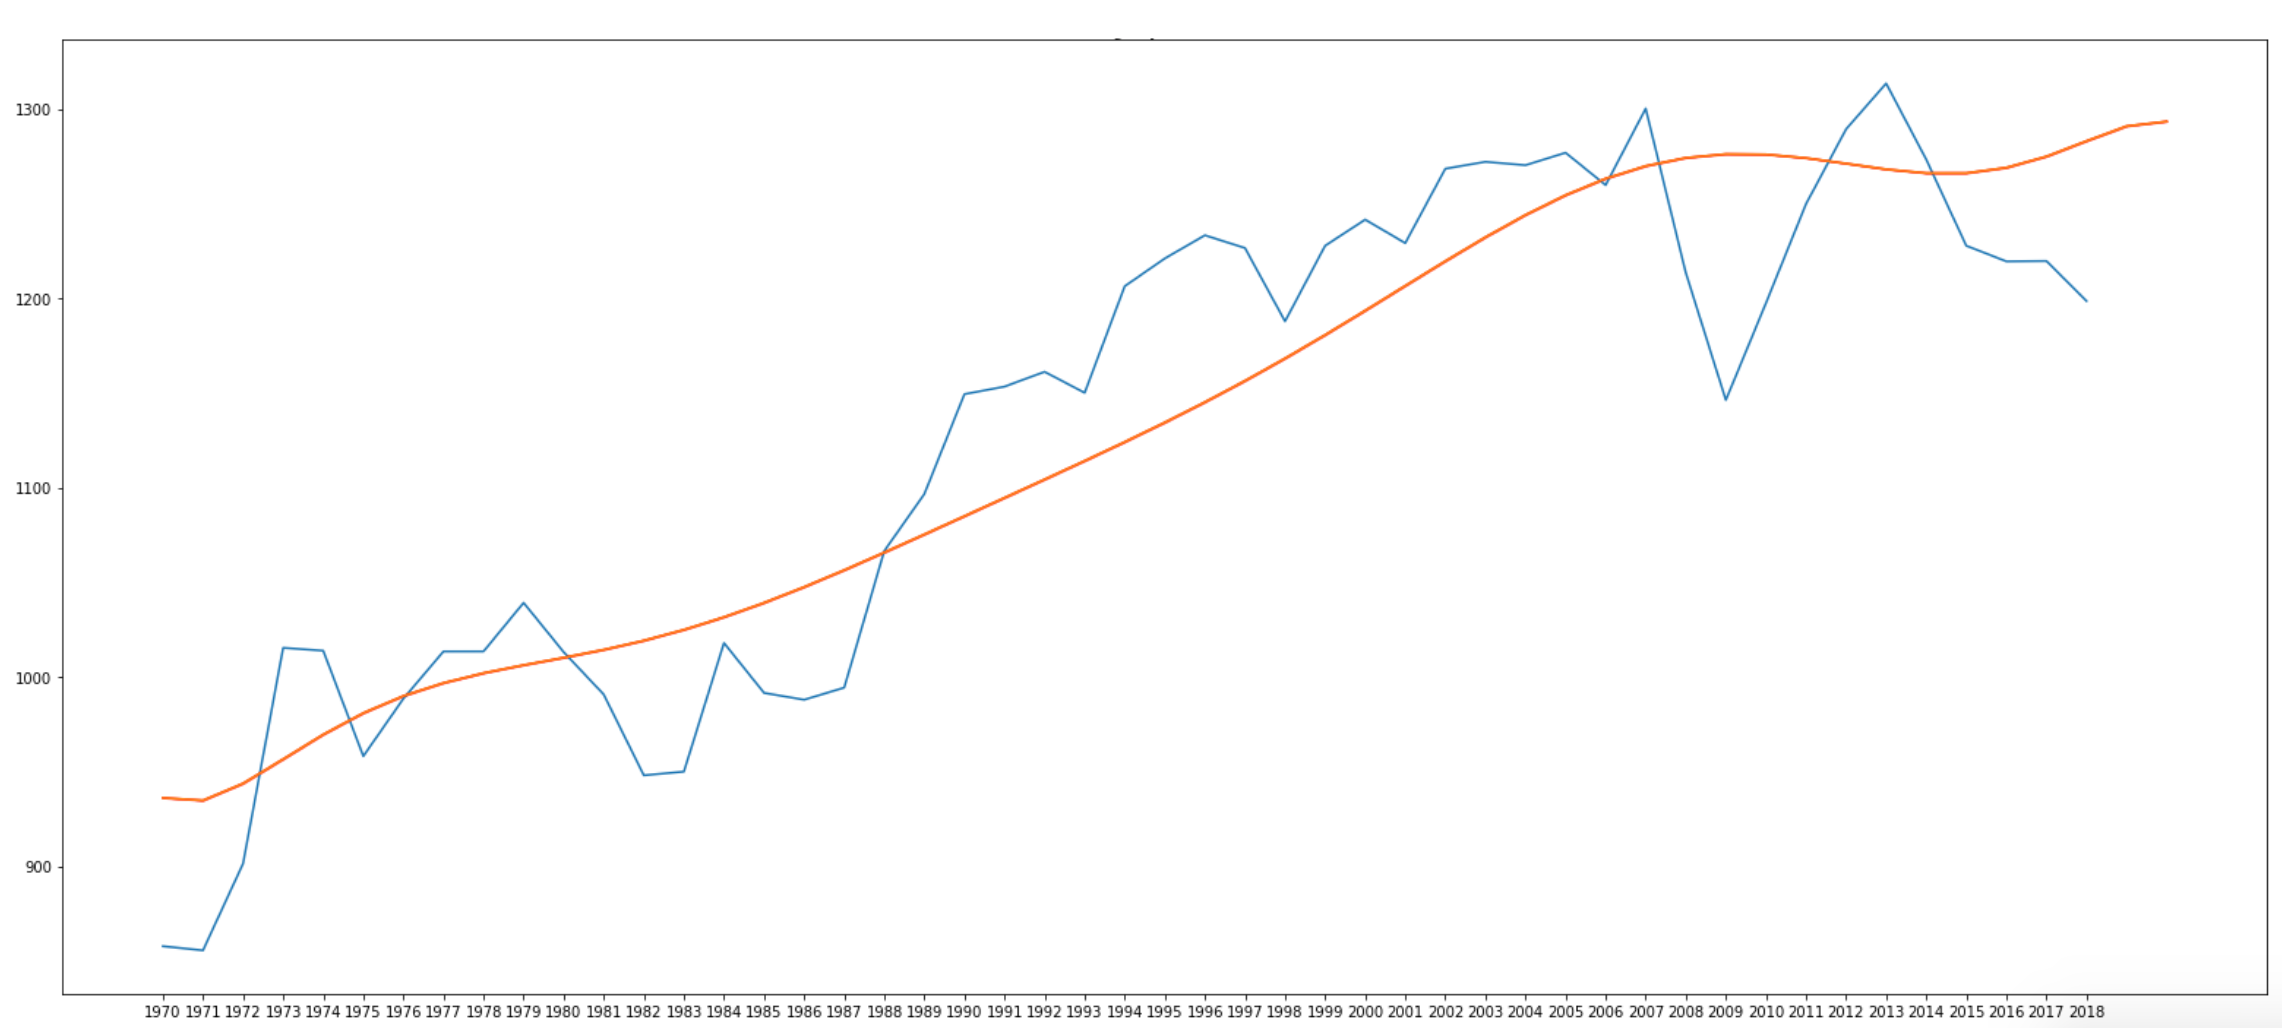
\includegraphics[width=0.5\linewidth]{ziedPNGS/3}}
	\subfloat[China]{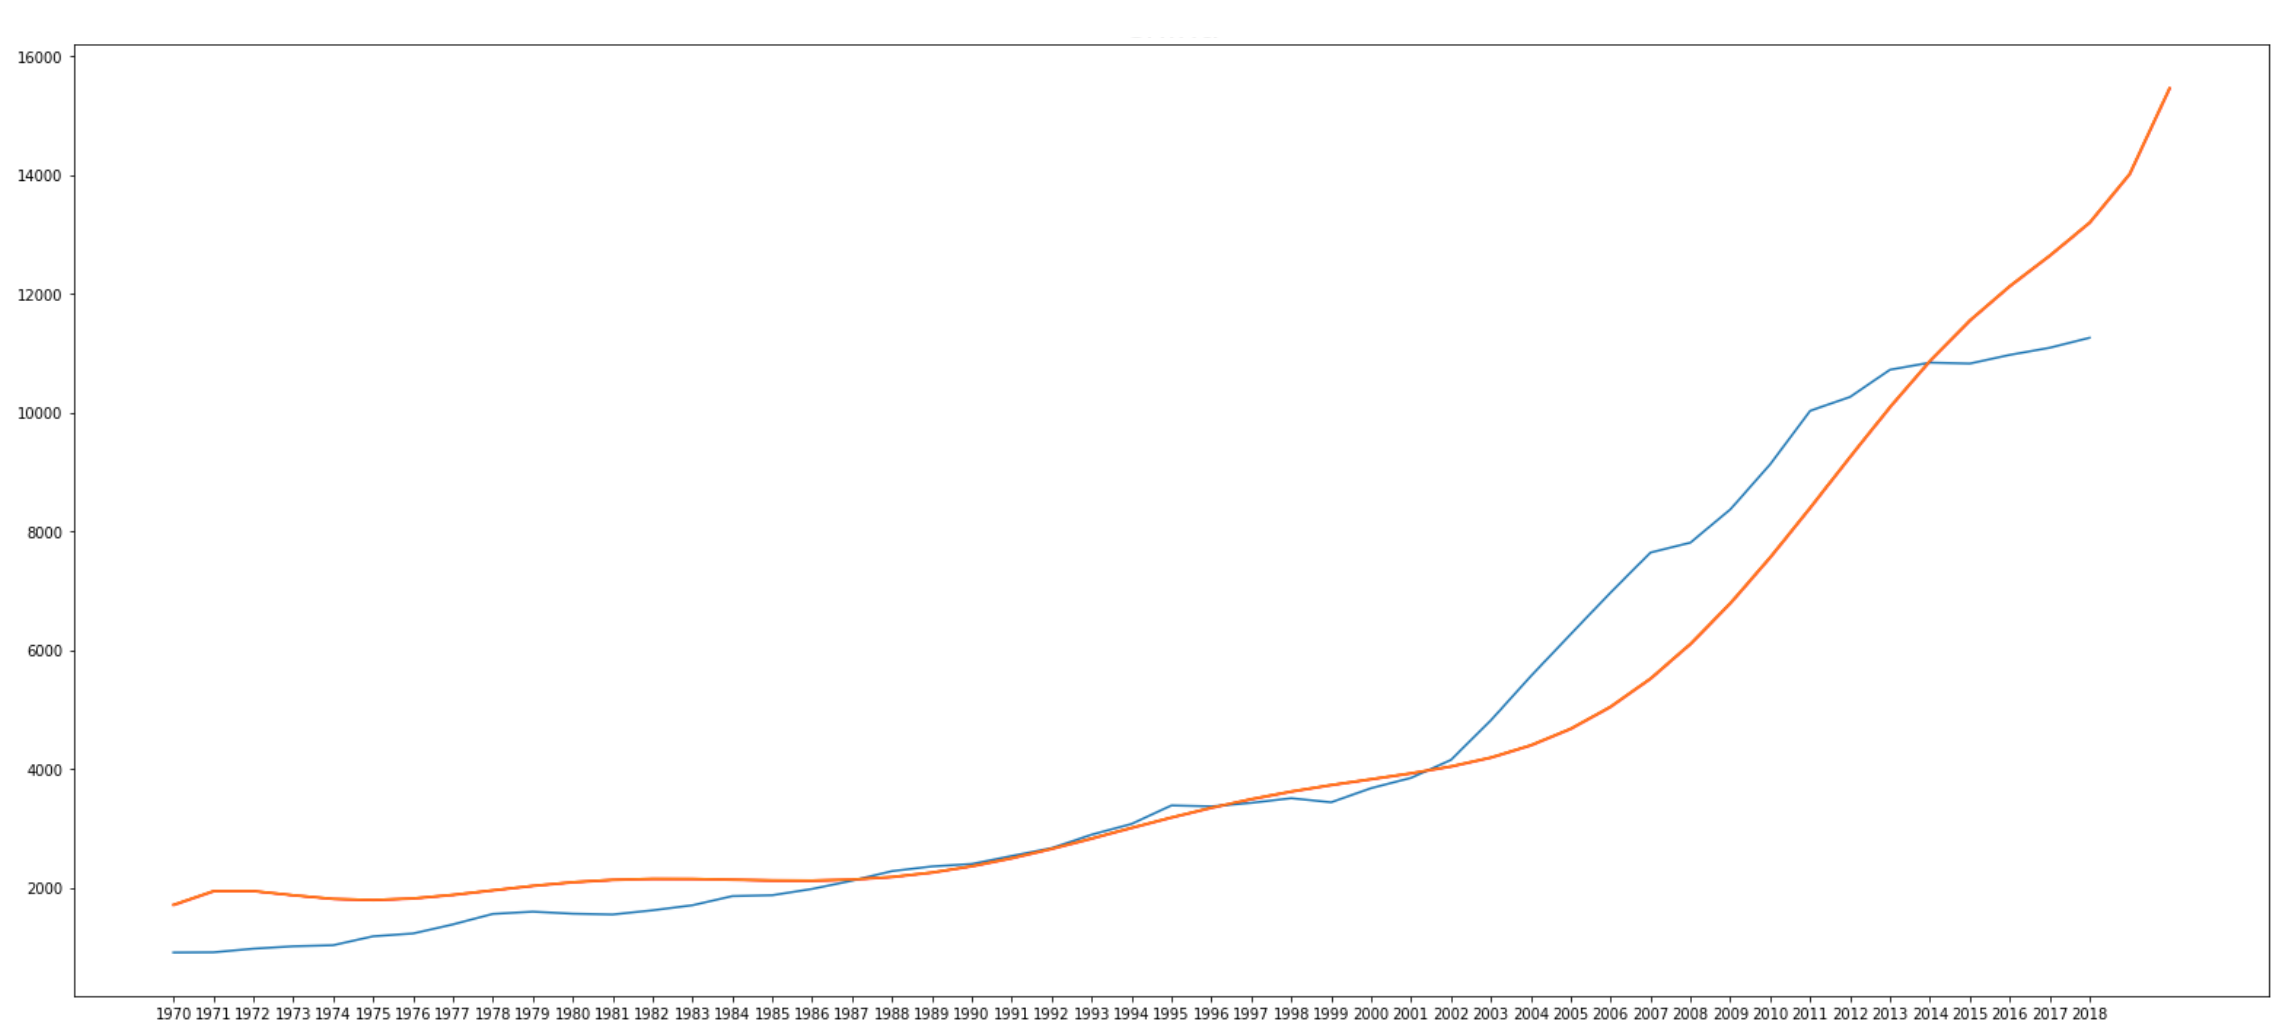
\includegraphics[width=0.5\linewidth]{ziedPNGS/4}}
	
	\subfloat[EU]{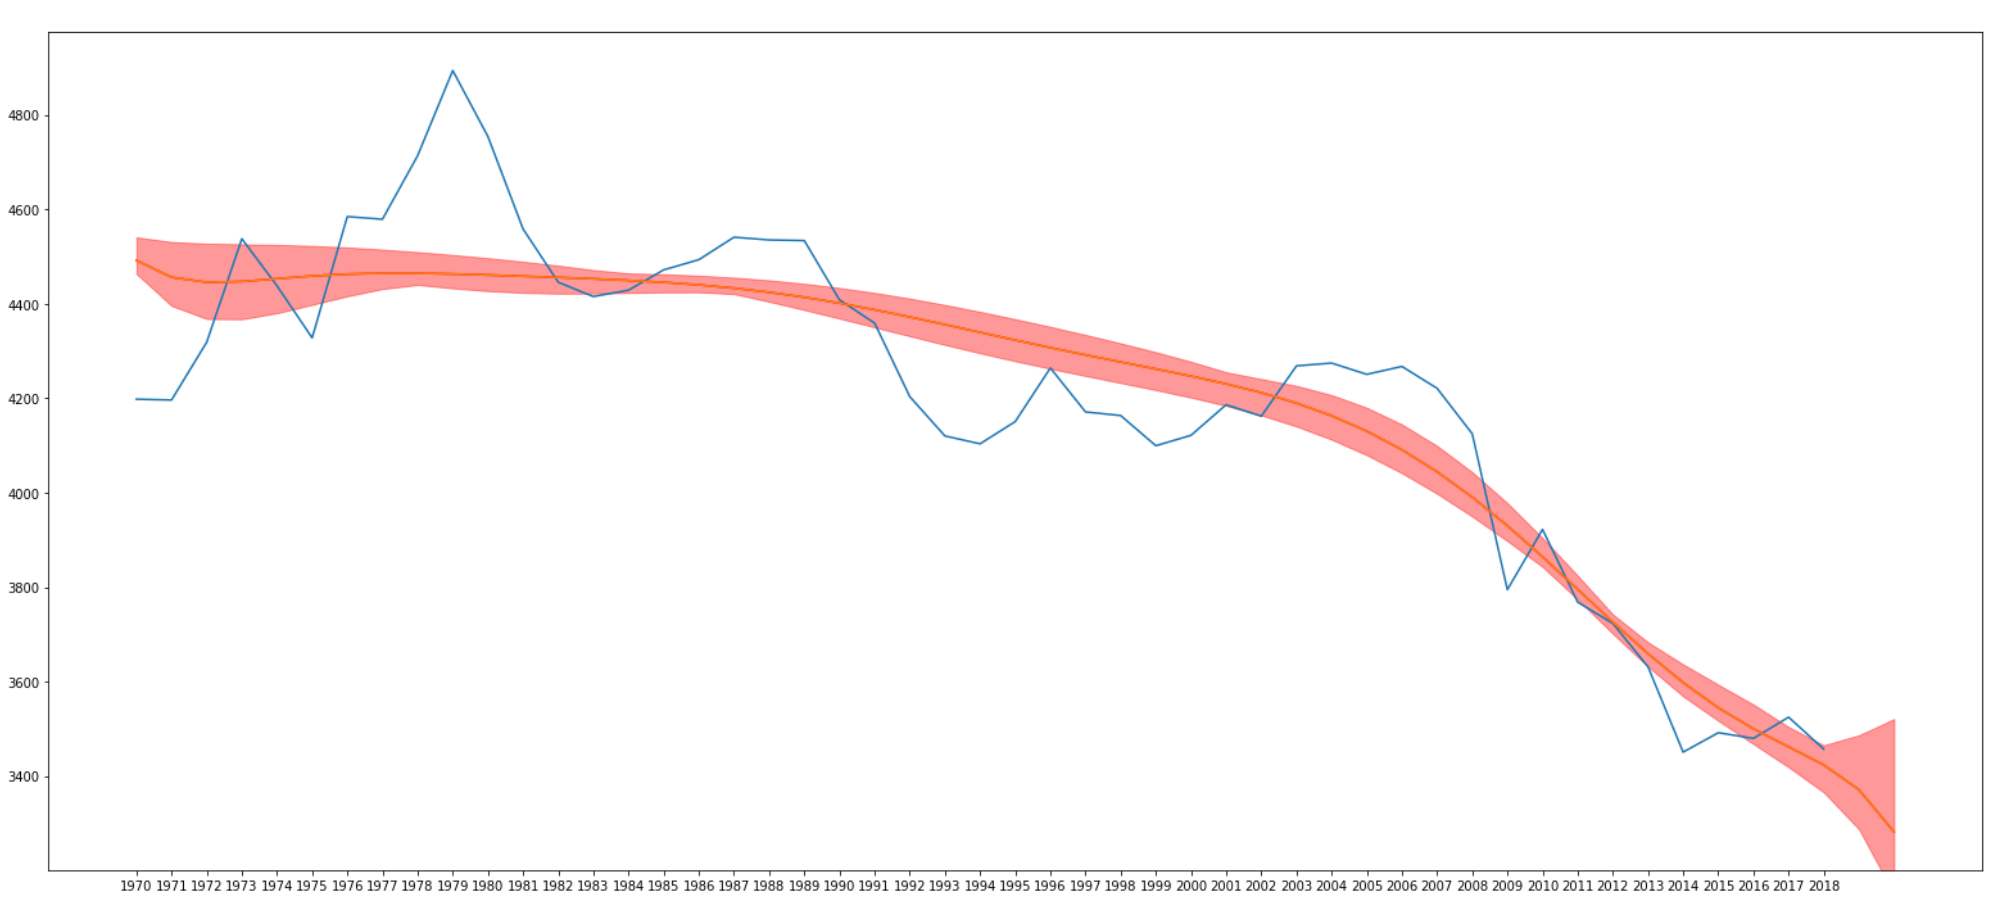
\includegraphics[width=0.5\linewidth]{ziedPNGS/5}}
	\subfloat[United States]{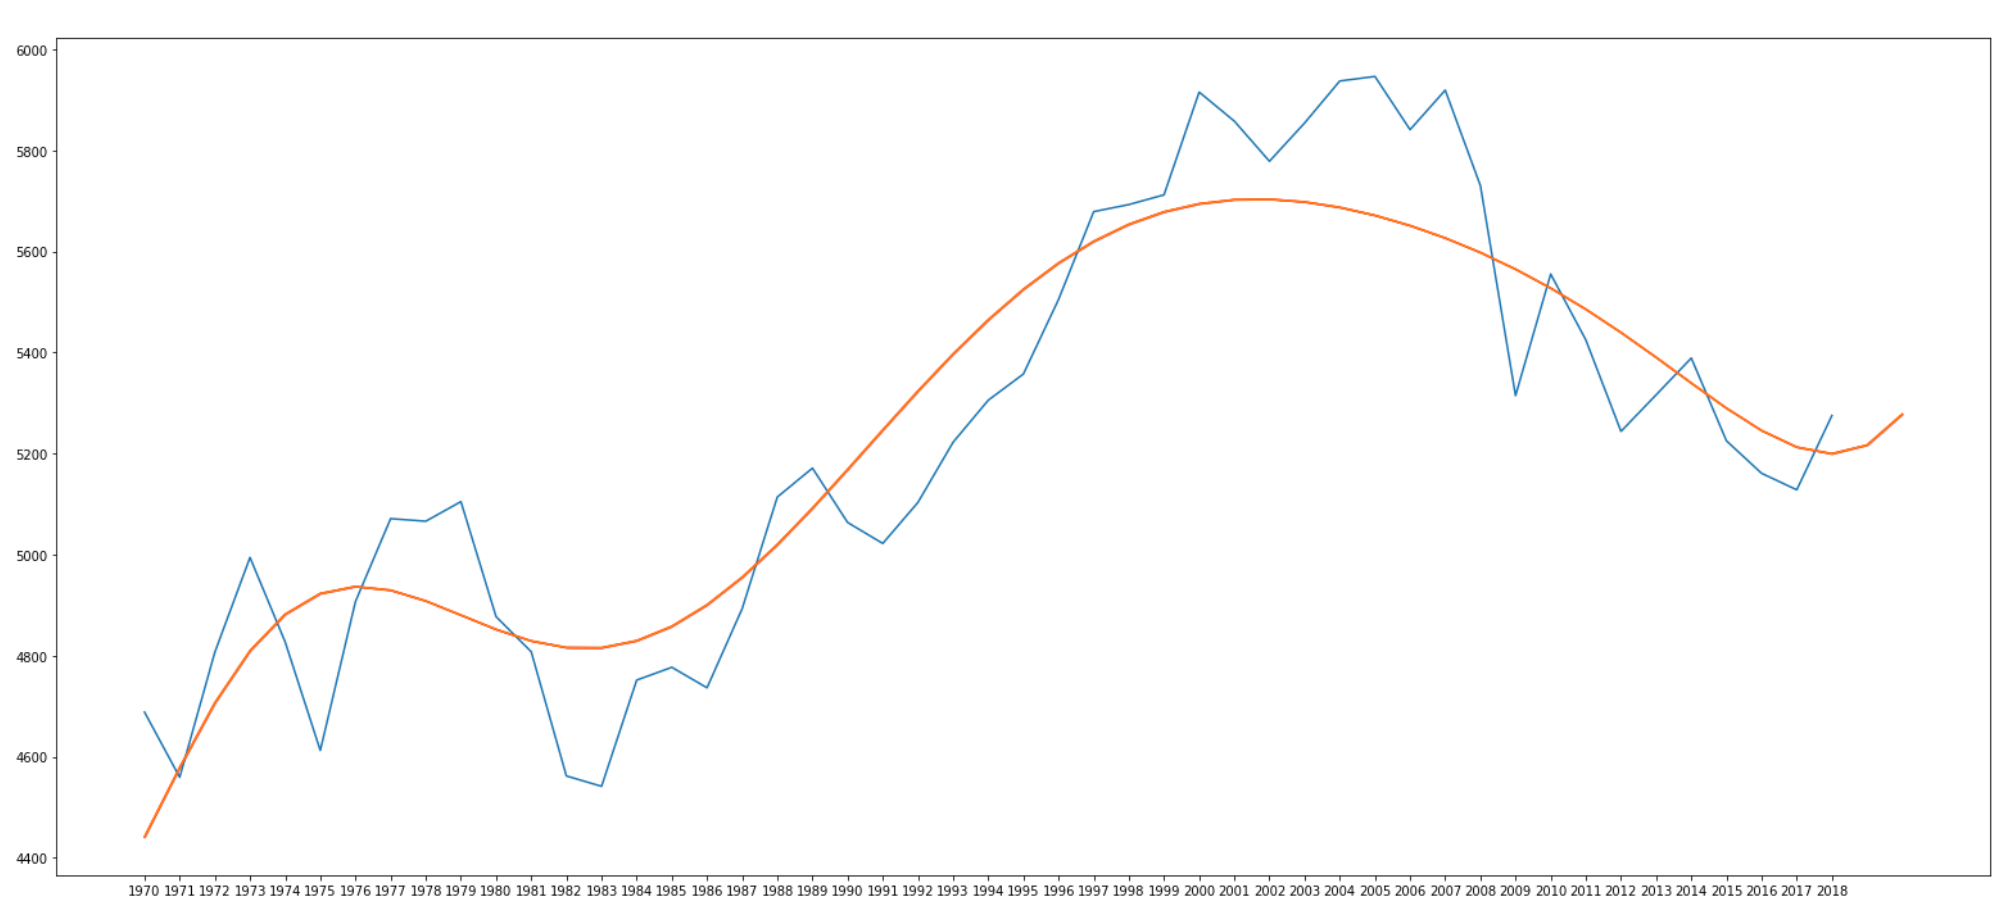
\includegraphics[width=0.5\linewidth]{ziedPNGS/6}}
	
	\subfloat[India]{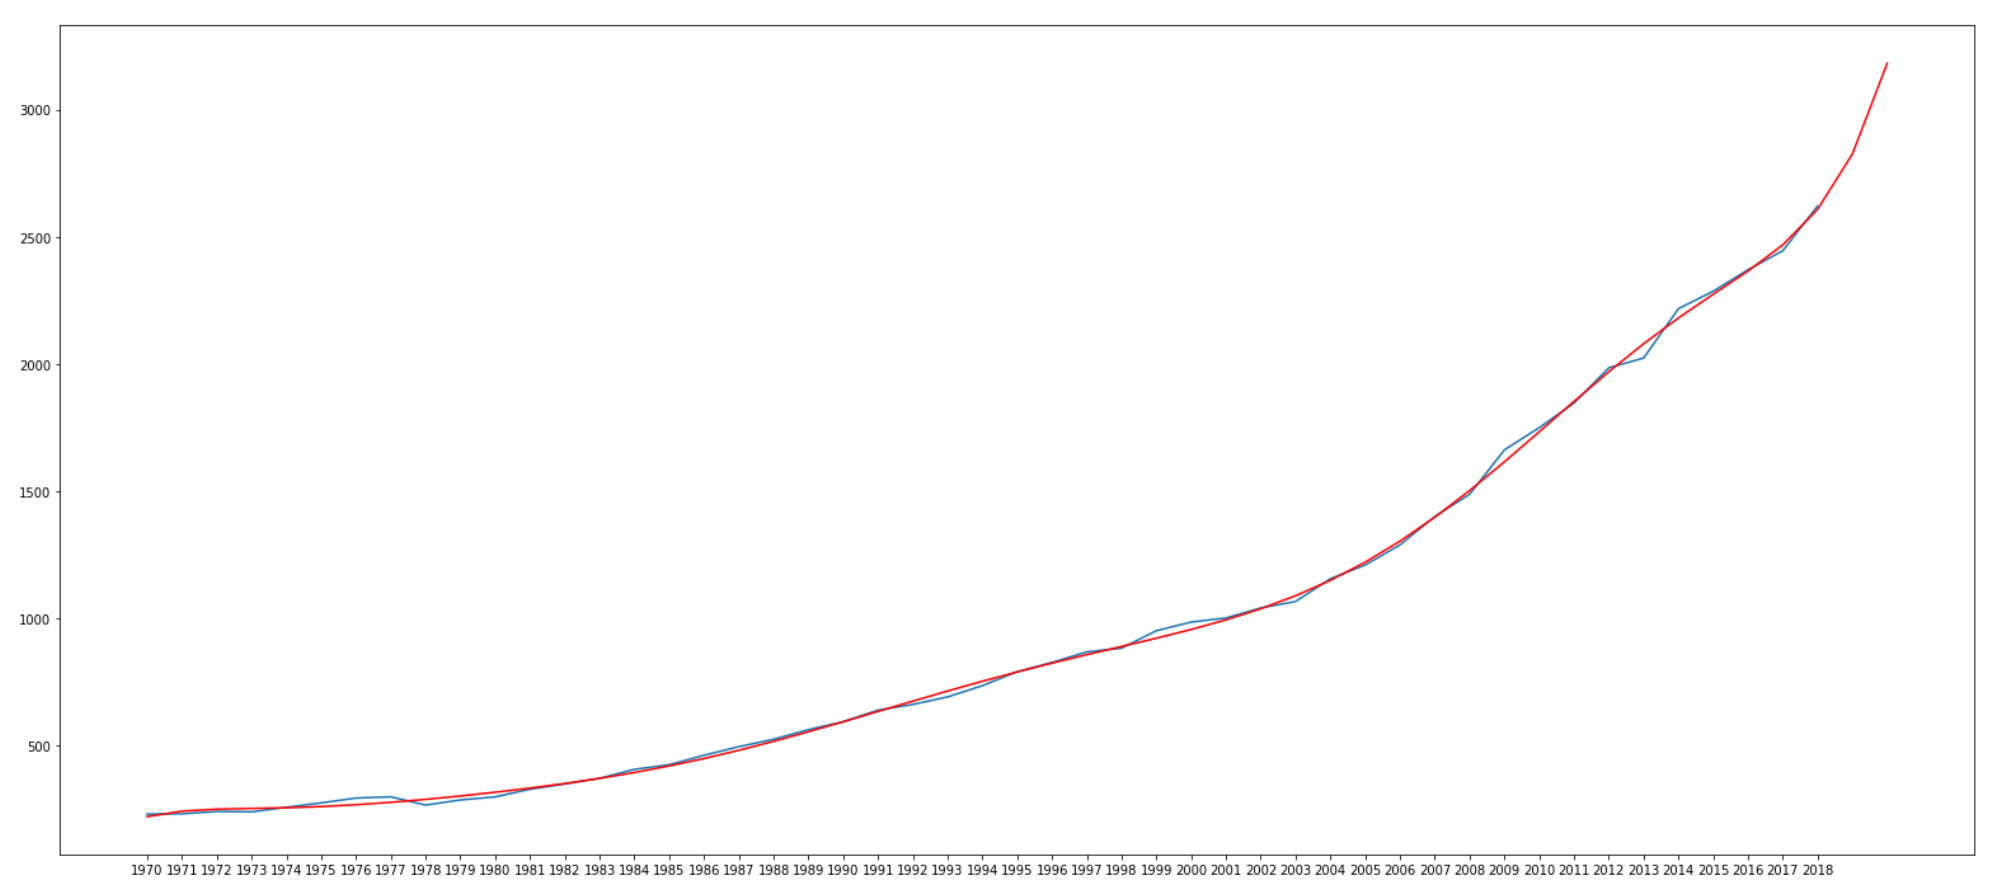
\includegraphics[width=0.5\linewidth]{ziedPNGS/7}}
	\caption{These graphs present the predicted emissions.}
	\label{fig:Results}
\end{figure}


%%%%%%%%%%%%%%%%%%%%%%%

\subsection{Sector indicators}

From the \co data we predicted for 2020 without considering COVID-19, we now want to deduce actual \co for this year. As monthly \co emission data is not available, we needed to find a way to model the emissions during the lock-down.
\co emissions can be split up in five major sectors, as depicted in \autoref{tab:sector_contributions}. For each sector, we know the yearly behavior but not the monthly. In this section, we will focus on finding monthly data for each sector.

\begin{table}[h!]%todo: Pie chart?, Values add up to 109 \% sadly
	\centering
	\begin{tabular}{lr}
		\hline
		Sector & Contribution to total emissions in 2018\\
		\hline
		\hline
		Power industry &  \(39.42\%\)\\ 
		Buildings &   \(10.90\%\)\\ 
		Mobility &   \(23.92\%\)\\ 
		Other industrial combustion &   \(22.30\%\)\\ 
		Other sectors &   \(12.56\%\)\\ 
		\hline &\\
	\end{tabular}
	\caption{All five majors sectors  and their contributions to the total \co emissions. Calculated from the EDGAR dataset.}%todo: source
	\label{tab:sector_contributions}	
\end{table}	



Knowing each sectors usual contribution to the total emissions, we want to find the behavior of the \co emissions of each sector during the lock-down. To do so, we use monthly data available to us that can be seen as an indicator for the respective sector. For each country, we extract one value per month in 2020 that we apply to our estimated 2020 \co emission data without considering COVID-19. In conclusion, we modulate our yearly data with monthly values to obtain monthly \co emission data for 2020.

\subsubsection{Power Industry}
The classification by sectors is given by the report of EDGAR \cite{crippa2019fossil}. The emissions produced by this sector refer to power and heat generation plants (public \& autoproducers). In a general view, it is the main source of greenhouse gas emissions. The original data from this sector is until 2018 and annual, so we cannot appreciate the impact of COVID-19. We decided to explore some indicators which were monthly updated to get an intuition. 


\paragraph{Indicators}
\begin{itemize}
	\item \textbf{Natural gas prices:} \cite{gas} dataset contains monthly and daily prices of natural gas, starting from January 1997 to current year. Prices are in nominal dollars.
	\item \textbf{Brent spot prices:} \cite{brent} Europe Brent and WTI (Western Texas Intermediate) Spot Prices (Annual/ Monthly/ Weekly/ Daily) from EIA U.S. (Energy Information Administration).
	\item \textbf{Electricity, gas, steam and air conditioning supply:} \cite{production} industry production per European country.
	\item \textbf{Supply oil:} \cite{production} as the previous reference, it is defined also per European country.
\end{itemize}

\paragraph{Strategy}
Due to the lack of monthly emission data for this sector which could show us the impact of COVID-19, we had to based our predictions in these indicators.

The first approach was to modulate the annual emissions with an indicator, in order to get monthly resolution. We could get the weights for each month in the indicator and apply it to the emissions. Then, we could apply machine learning to predict the emissions using indicators, what would be our data considering COVID-19 against the time series prediction of the emissions which represents the data without considering COVID-19. The problem is we were using twice the same data (an indicator), first to modulate the emissions and then to train the model.

For this reason we chose to change the strategy. Now the procedure was to find the most correlated indicator per each country between these four (consider that for non European countries we only have the natural gas and brent prices). Then, we assume the emissions behave as the selected indicator and we are able to identify if there is any change, comparing the real values of the indicator with a time series prediction from previous months affected by COVID-19. The steps are the following:

\begin{enumerate}
	\item \textbf{Selection of most correlated indicator:} we looked for only one indicator per country which could explain the behavior of the emissions. 
	\item \textbf{Time series prediction from december of 2019:} we predict the last months when the COVID-19 had not a big impact, in order to have a reference to compare. The prediction was using the SARIMA model \cite{sarima}. 
	\item \textbf{Extracting COVID-19 influence:} as we have current data from the last months (from January to May of 2020), we can observe a relative change respect the predicted values.
\end{enumerate}


\paragraph{Results}
Depending on the country we are studying, the obtained correlation is very different. 

In Figure \ref{fig:indicators_EEUU_China} we have two cases with only two indicators: United States and China. In the first one we got a correlation larger than 0.8, while in China it does not reach 0.1.
\begin{figure}[h!]
	\centering
	\subfloat[United States]{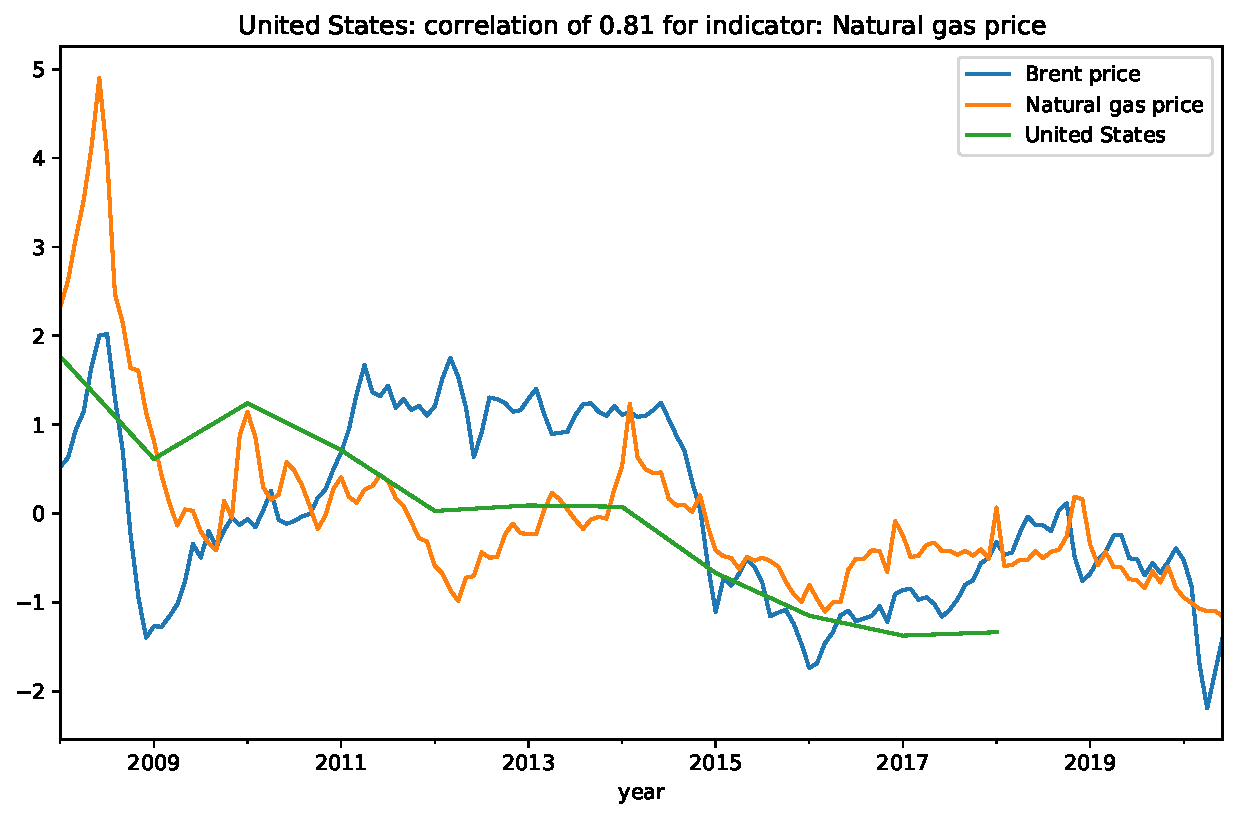
\includegraphics[width=0.5\linewidth]{../power_industry/United States_indicators}}
	\subfloat[China]{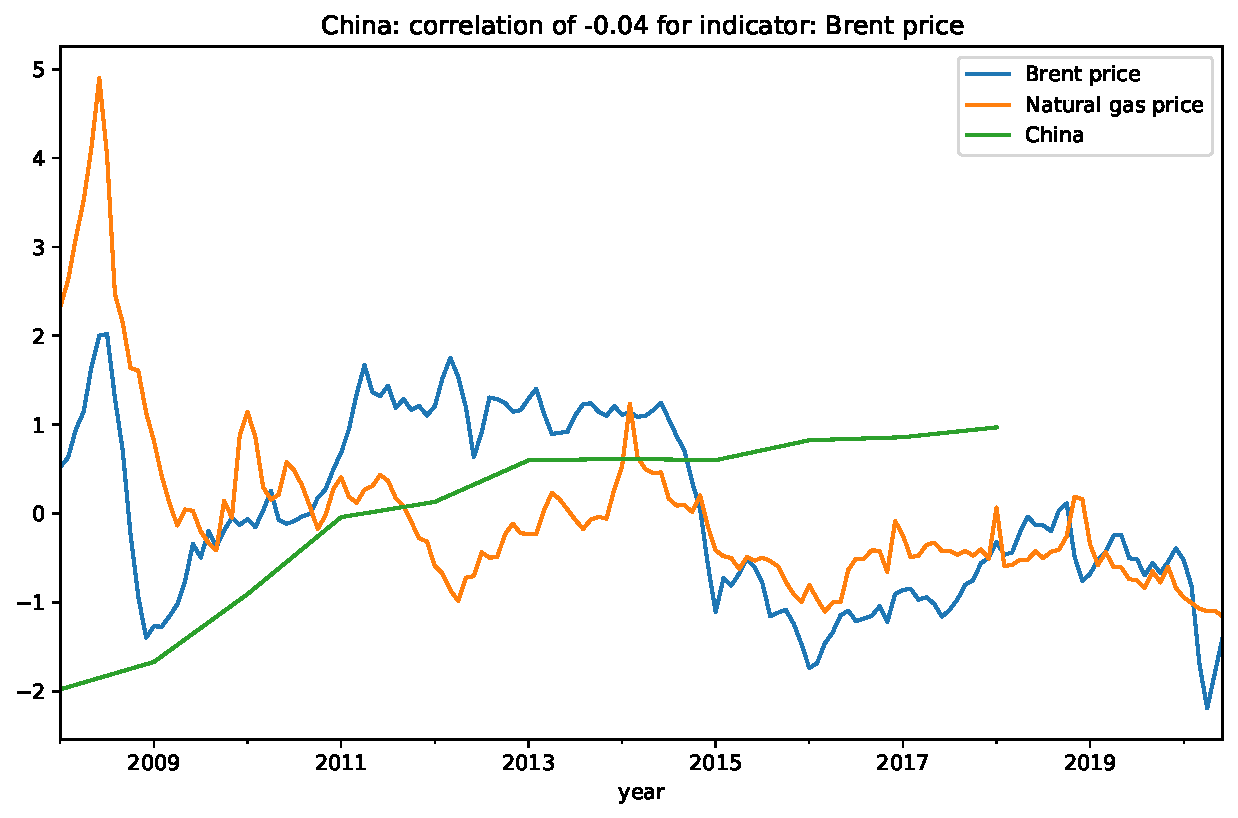
\includegraphics[width=0.5\linewidth]{../power_industry/China_indicators}}
	\caption{Indicators and annual emissions for non European countries.}
	\label{fig:indicators_EEUU_China}
\end{figure}

The same behavior appears in European countries where we have 4 indicators as it is shown in the Figure \ref{fig:indicators_Denmark_Portugal}
\begin{figure}[h!]
	\centering
	\subfloat[Denmark]{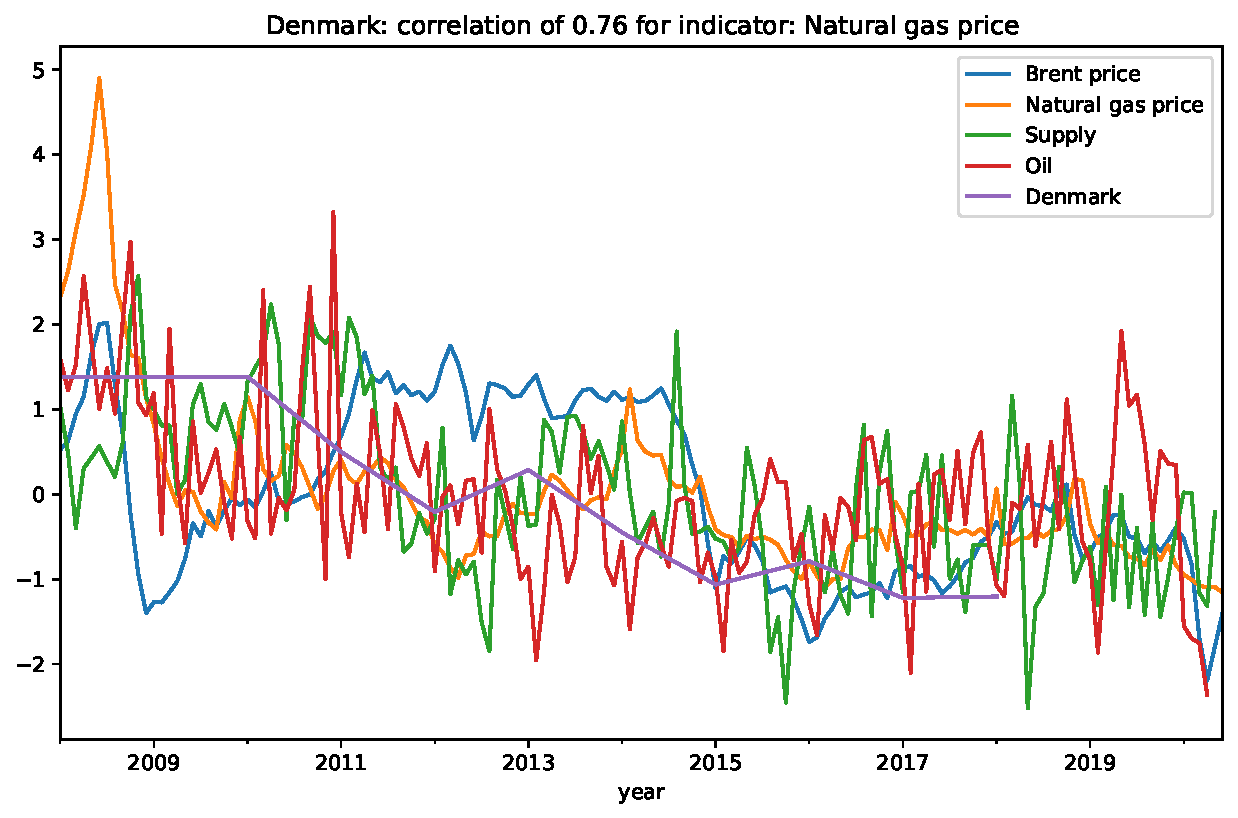
\includegraphics[width=0.5\linewidth]{../power_industry/Denmark_indicators}}
	\subfloat[Portugal]{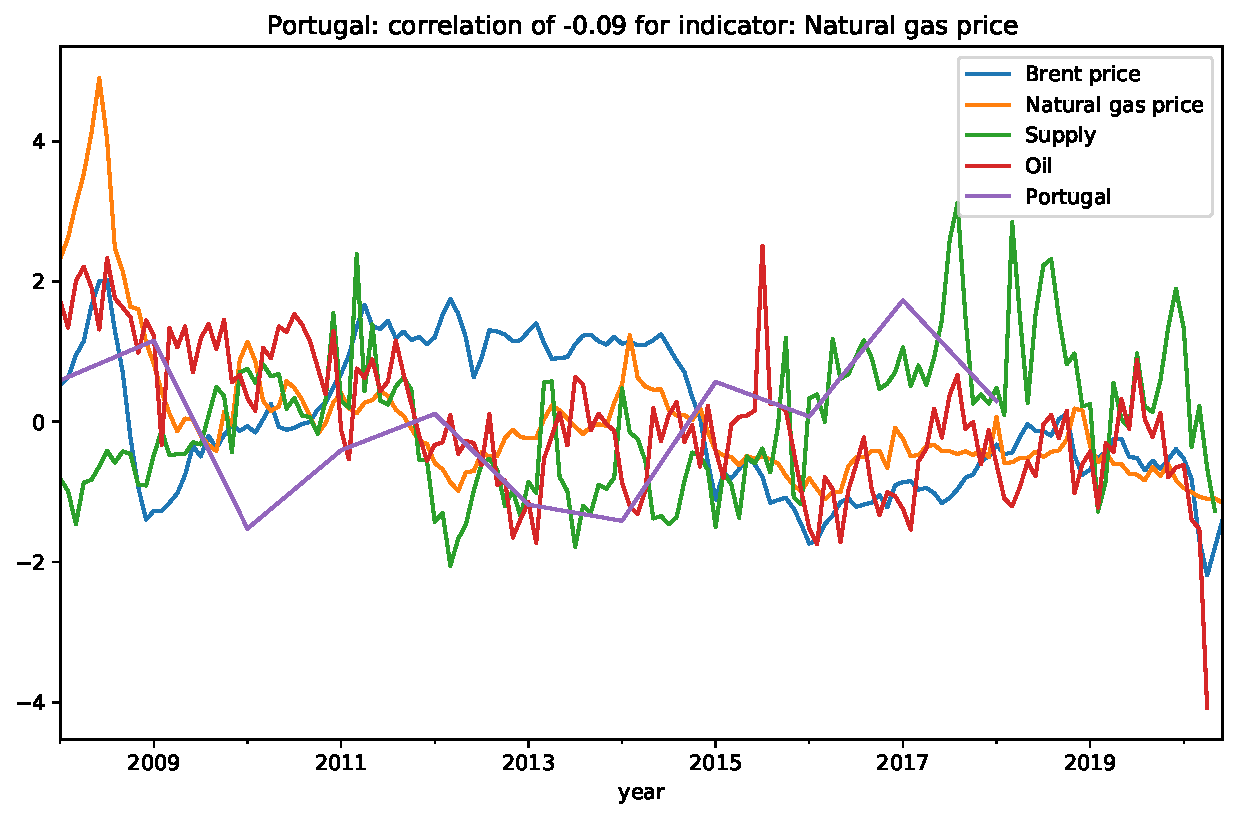
\includegraphics[width=0.5\linewidth]{../power_industry/Portugal_indicators}}
	\caption{Indicators and annual emissions for European countries.}
	\label{fig:indicators_Denmark_Portugal}
\end{figure}

In Table \ref{table:correlation} we can observe the selected indicators and the respective correlation with the emissions for the 8 biggest contributors in emissions.
\begin{table}[h!]
	\centering
	\begin{tabular}{ccc}
		\hline
		Country & Correlation Indicator \& Emissions & Selected Indicator \\
		\hline
		\hline 
		EU & 0.740 & Brent Price \\
		United States & 0.813 & Natural Gas Price \\
		India & -0.272 & Brent Price \\
		China & -0.038 &  Brent Price \\
		Japan &  0.428 & Brent Price \\
		Russia & 0.792 & Brent Price \\
		Canada & 0.785 & Natural Gas Price \\
		Brazil & 0.021 & Brent Price\\
		\hline 
		&& \\
	\end{tabular}
	\caption{Resulting correlations for the biggest contributors}
	\label{table:correlation}  
\end{table}

Once the indicator is selected, SARIMA model is applied per country, allowing us to check if there is a relative change in this indicator and simultaneously to $ CO_2 $ emissions. The results are plotted in Figure \ref{fig:sarima}. 
\begin{figure}[h!]
	\centering
	\subfloat[European Union]{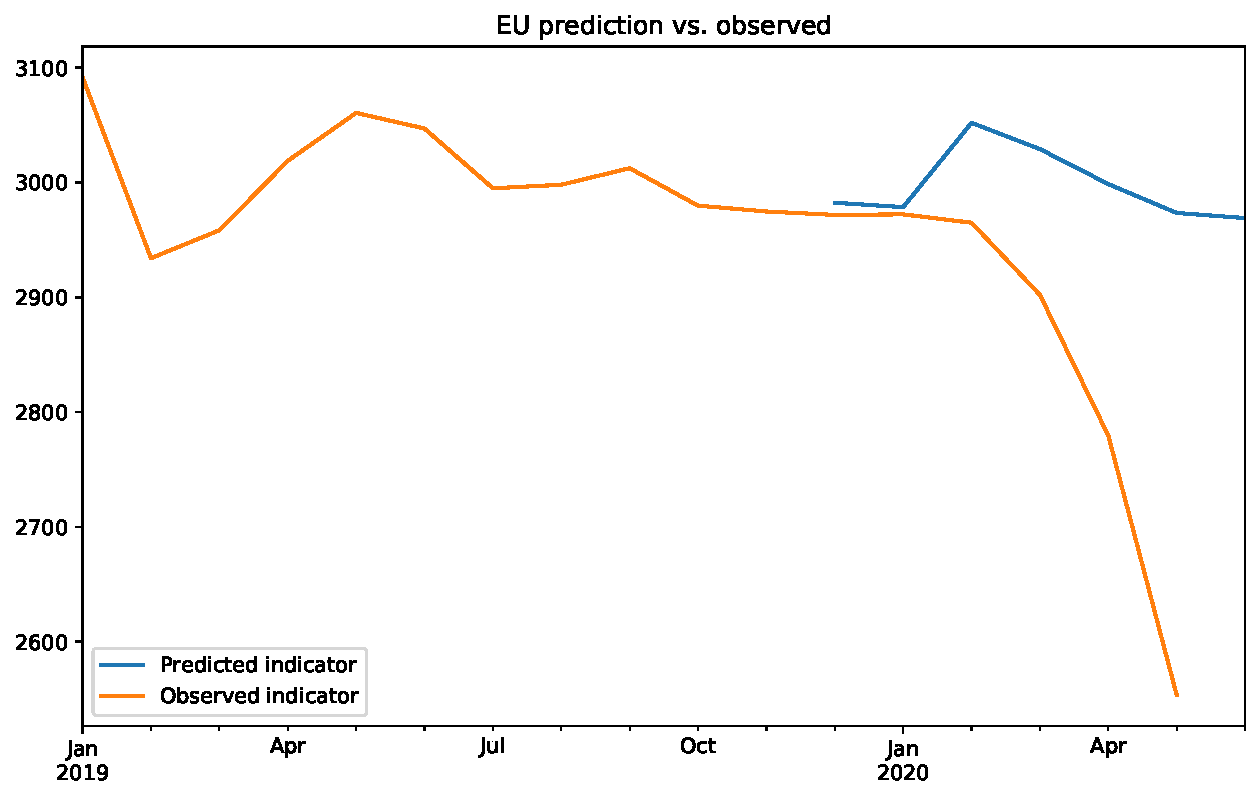
\includegraphics[width=0.4\linewidth]{../power_industry/EU_prediction}}
	\subfloat[United States]{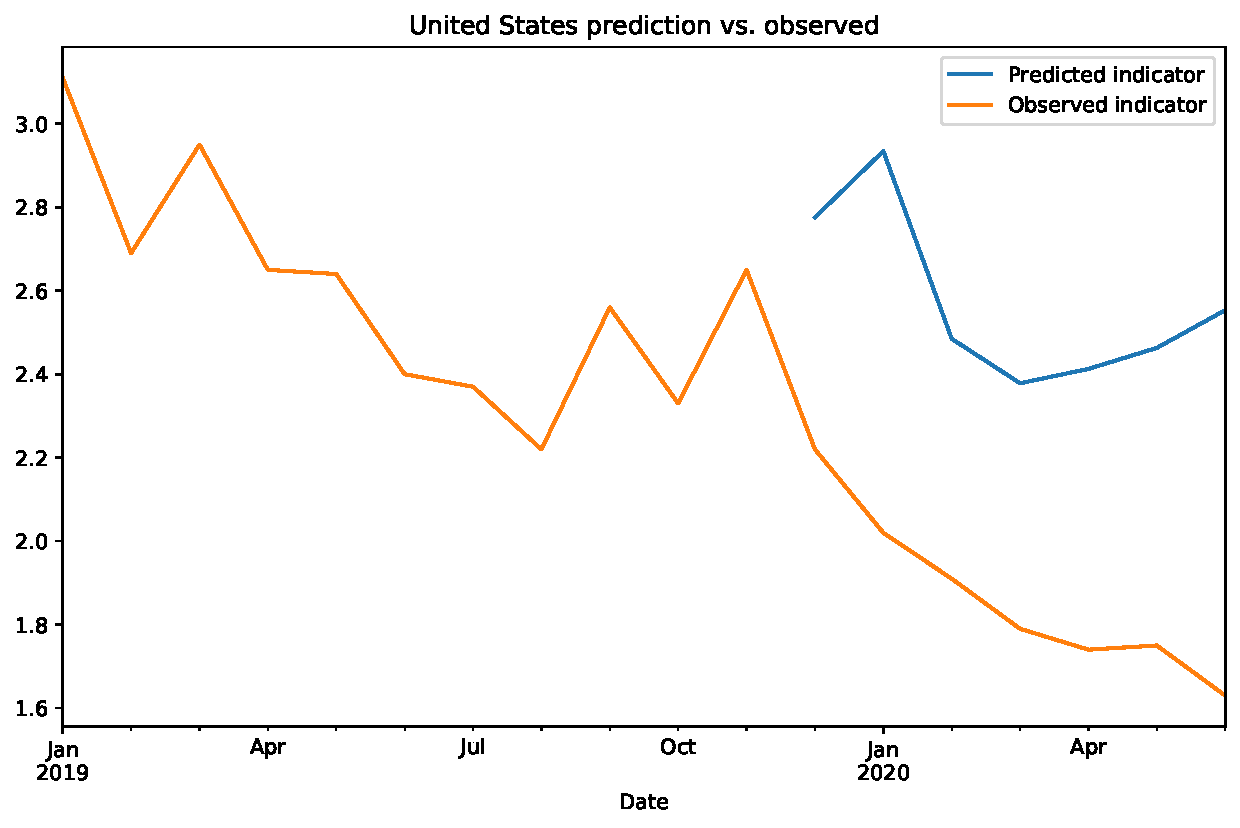
\includegraphics[width=0.4\linewidth]{../power_industry/United States_prediction}} \\
	\subfloat[India]{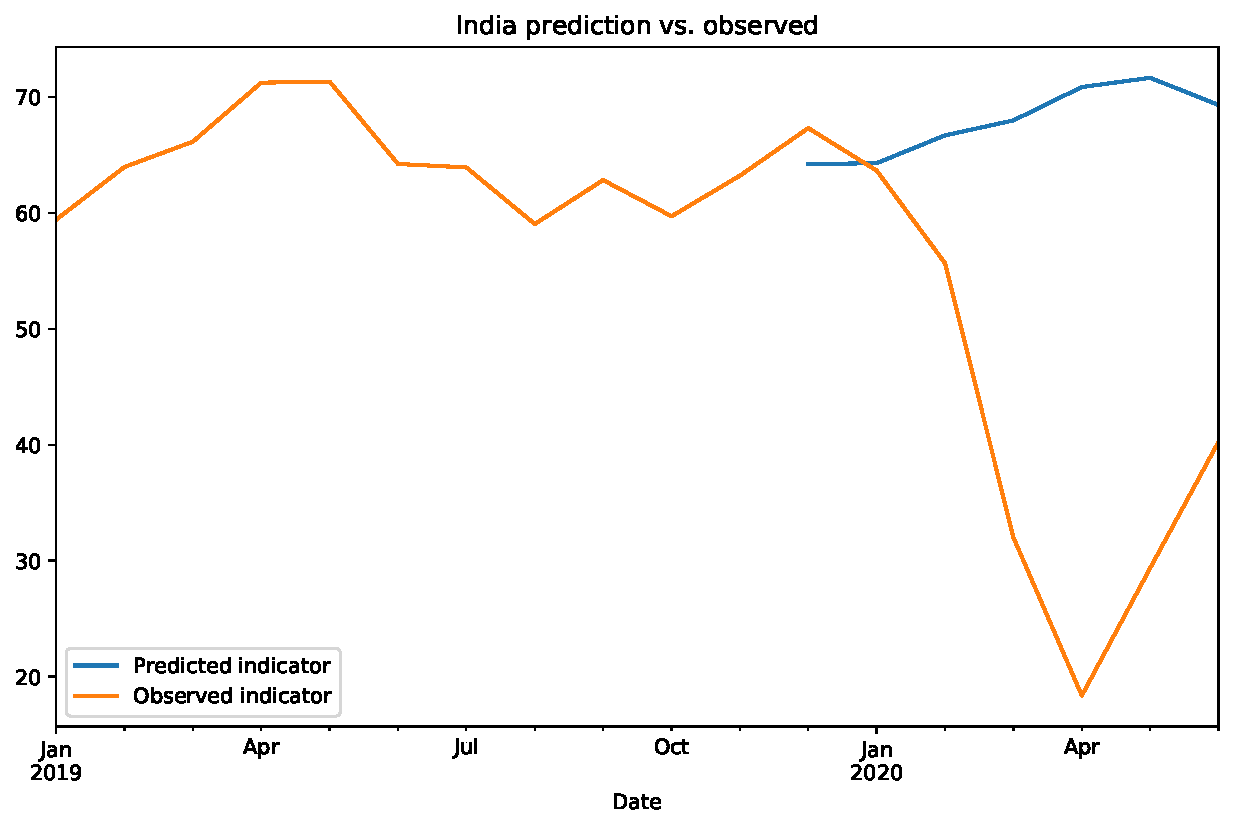
\includegraphics[width=0.4\linewidth]{../power_industry/India_prediction}}
	\subfloat[China]{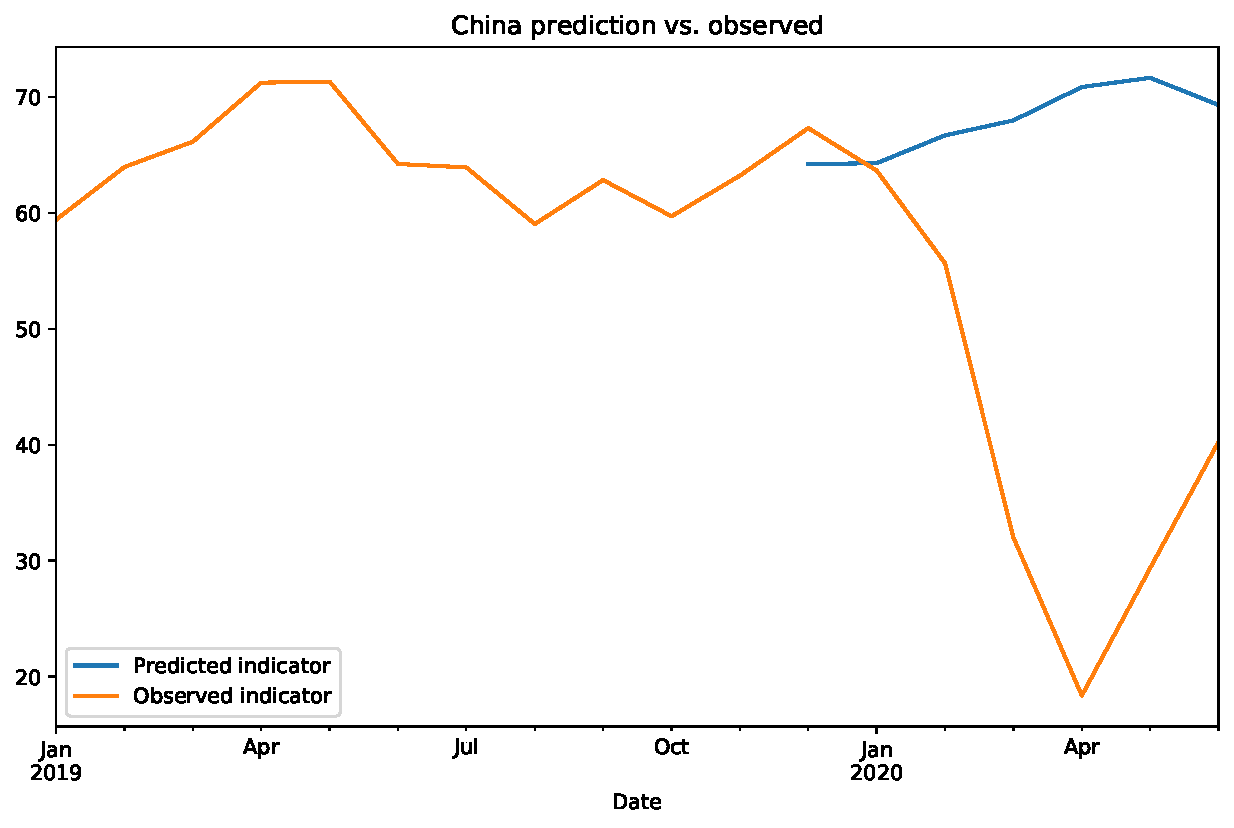
\includegraphics[width=0.4\linewidth]{../power_industry/China_prediction}} \\
	\subfloat[Japan]{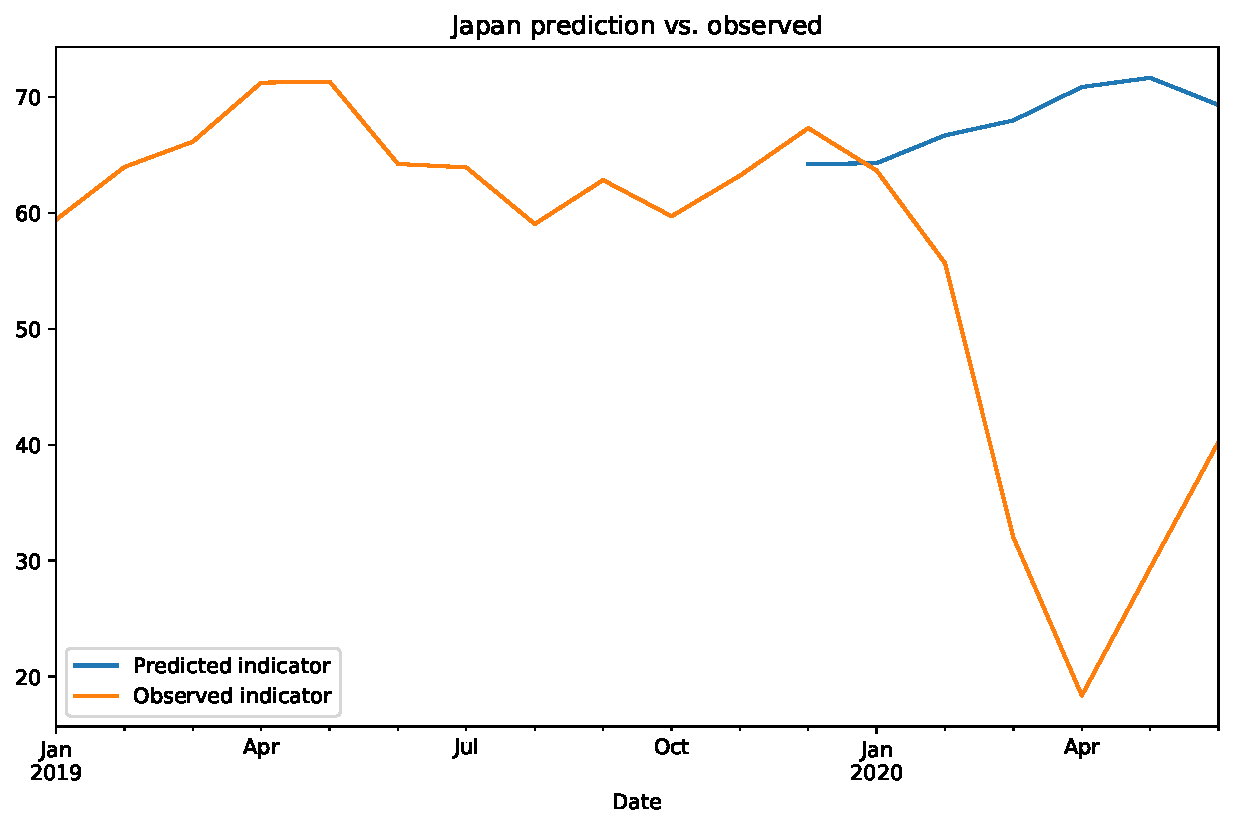
\includegraphics[width=0.4\linewidth]{../power_industry/Japan_prediction}}
	\subfloat[Russia]{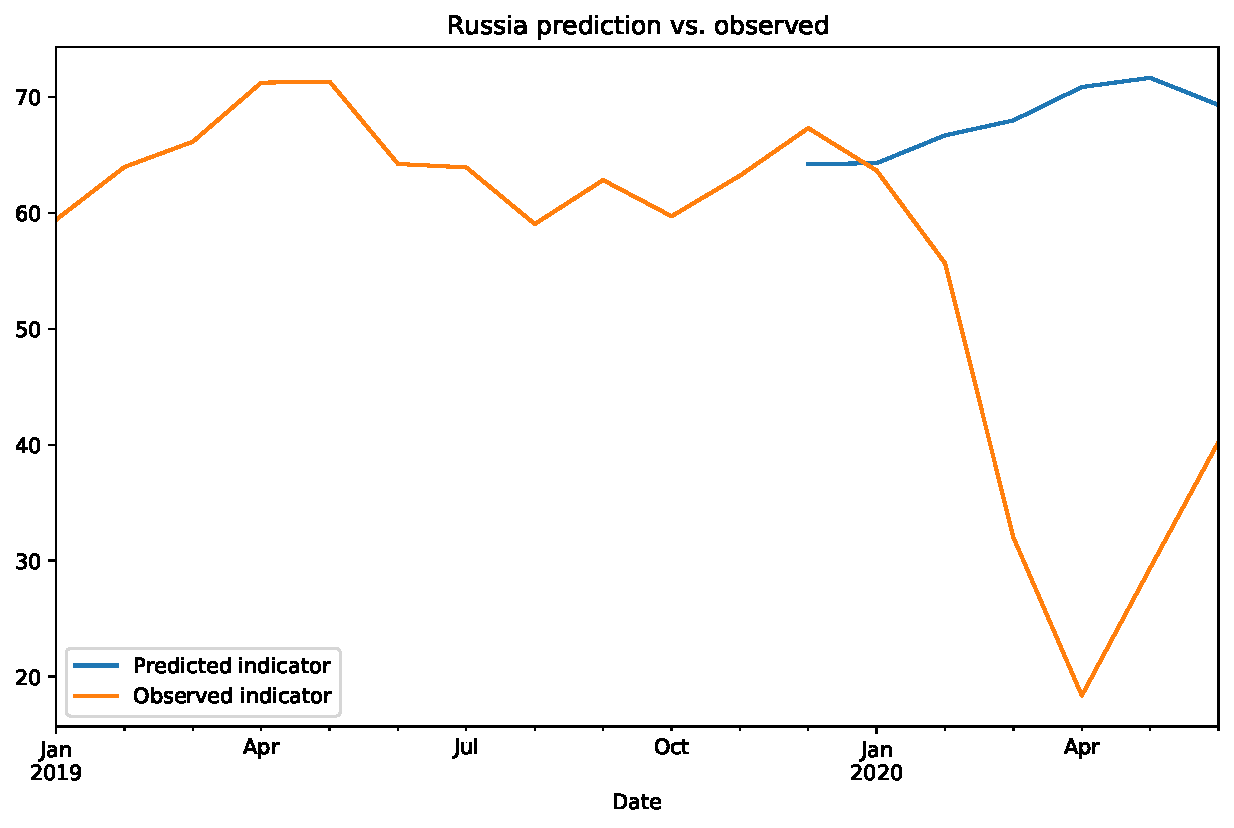
\includegraphics[width=0.4\linewidth]{../power_industry/Russia_prediction}} \\
	\subfloat[Canada]{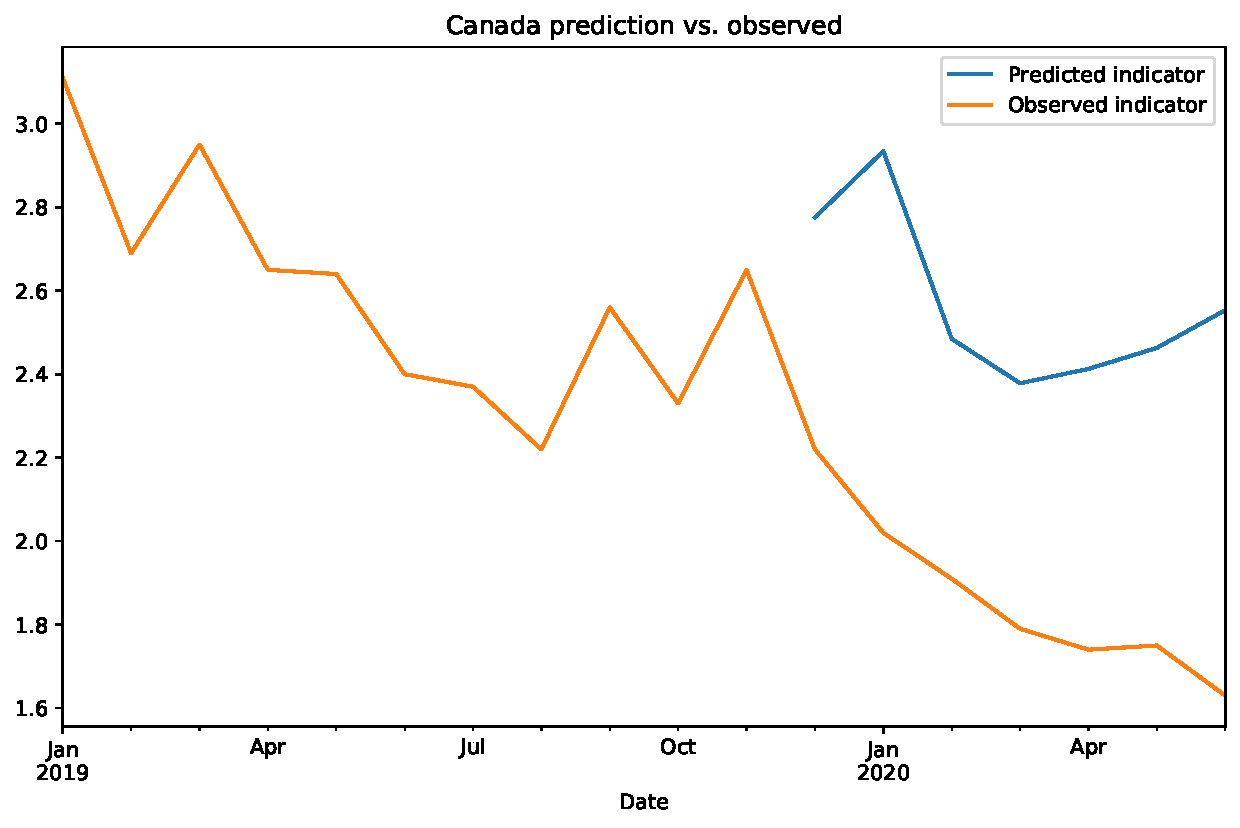
\includegraphics[width=0.4\linewidth]{../power_industry/Canada_prediction}}
	\subfloat[Brazil]{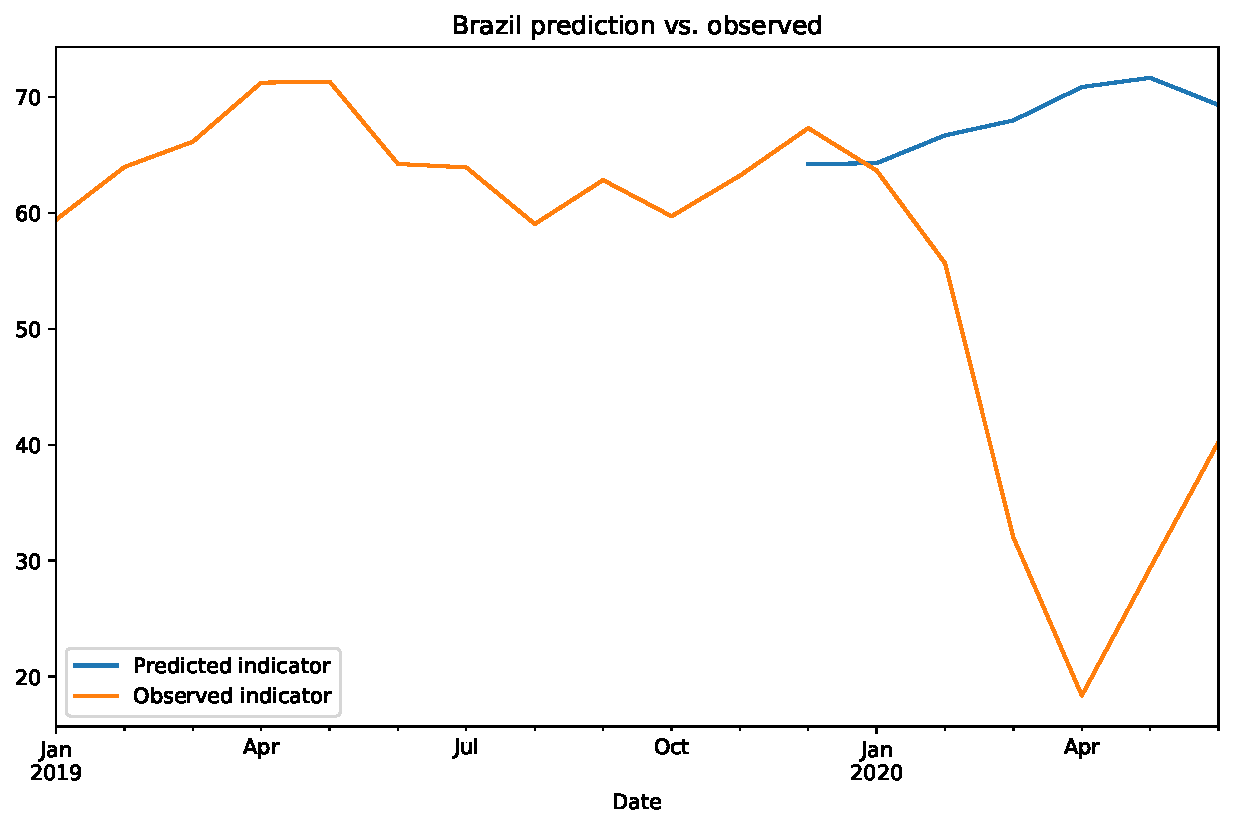
\includegraphics[width=0.4\linewidth]{../power_industry/Brazil_prediction}}
	\caption{Predicted vs real values of selected indicators.}
	\label{fig:sarima}
\end{figure}

In Table \ref{table:change} we show the rate of change for the months we have data. This ratio can be described as:

\begin{equation}
	\text{Rate} = \frac{\text{indicator considering COVID-19}}{\text{indicator without considering COVID-19}} = \frac{\text{actual value of the indicator}}{\text{prediction of the indicator}} 
\end{equation}
\begin{table}[h!]
	\centering
	\begin{tabular}{c|cccccccc}
		\hline
		Country & European Union & United States & India & China & Japan & Russia & Canada & Brazil \\ 
		\hline 
		December, 2019 & 0.996 & 0.800 & 1.048 & 1.048 & 1.048 & 1.048 & 0.800 & 1.048  \\
		January, 2020 & 0.998 & 0.688 & 0.990 & 0.990 & 0.990 & 0.990 & 0.688 & 0.990 \\
		February, 2020 & 0.971 & 0.769 & 0.835 & 0.835 & 0.835 & 0.835 & 0.769 & 0.835 \\
		March, 2020 & 0.958 & 0.752 & 0.471 & 0.471 & 0.471 & 0.471 & 0.752 & 0.471 \\
		April, 2020 & 0.927 & 0.721 & 0.259 & 0.259 & 0.259 & 0.259 & 0.721 & 0.259 \\
		May, 2020 & 0.859 & 0.710 & 0.410 & 0.410 & 0.410 & 0.410 & 0.710 & 0.410 \\
		June, 2020 & \textit{No data} & 0.638 & 0.581 & 0.581 & 0.581 & 0.581 & 0.638 & 0.581 \\
		\hline
	\end{tabular}
	\vspace{1em}
	\caption{Rate of change in the indicator.}
	\label{table:change}  
\end{table}

\paragraph{Conclusion}
Due to the lack of data in emissions of $ CO_2 $, the reliability in our assumptions is based in the correlation with an indicator. Consequently, there are countries which this relation is not very strong and the vector of rate change does not make any sense, since it does not show a reliable situation. 

As mentioned before, non European countries tend to have smaller correlations due to having only two global indicators. In contrast, countries which belong to Europa have four indicators, being two of them unique per country. In results we shown cases with good performance and others which are not optimal, regardless of the region.
\subsubsection{Buildings}
%Introduction
The emissions of the buildings sector is composed of stationary combustion and the construction of buildings. In 2018, it had an average contribution of 10.9\%
percent to the worlds greenhouse gas emissions. 
In this part, the goal was to make a monthly prediction of the 2020 emissions based on real time indicators that also were available long before the COVID-19 crisis in order to be able to correlate them.

%Materials and Methods
\paragraph{Indicators}

Sadly, the construction industry employment dataset was only updated until 2018, which is the reason why we chose to limit our datasets to the ones presented below:

\begin{itemize}
	\item \textbf{Producer price index by commodity for metals and metal producs: Iron Steel.}
	Source: Federal reserve Bank of St. Louis
	\url{https://fred.stlouisfed.org/series/WPU101}
	\item \textbf{Producer Price index by industry: cement and concrete product manufacturing.}
	Source:  Federal reserve Bank of St. Louis
	\url{https://fred.stlouisfed.org/series/PCU32733273}
	\item \textbf{Industrial Production: Durable Goods: Cement and concrete products.}
	Source:  Federal reserve Bank of St. Louis
	\url{https://fred.stlouisfed.org/series/IPG3273S}
	\item \textbf{Total construction spending.}
	Source:  Federal reserve Bank of St. Louis
	\url{https://fred.stlouisfed.org/series/TTLCONS}
\end{itemize}%todo: Were they all used? Spelling, Reduce info

The general idea was that the price should correlate with the demand for the product. Together with the assumption that the construction industry consumes a significant amount of the worlds concrete and steel production, the hypothesis is that we can use the prices as indicators in a machine learning model that is able to predict the emissions in 2020 based on previous price development.

In Figure \ref{fig:indicators}, selected indicators are plotted against the global \co emissions.
\begin{figure}[h!]
\centering
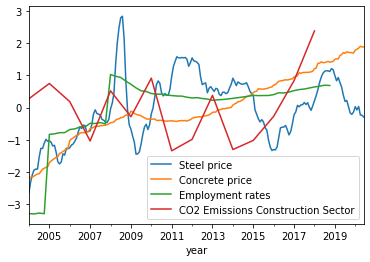
\includegraphics[width=0.4\linewidth]{../buildings/indicators}
\caption{Indicators and global \co emissions in arbitrary units.}
\label{fig:indicators}
\end{figure}
In general, one can observe that a slight correlation can already be seen on the global scale. of course, different countries are impacted differently from the prices. 
%todo: describe the raw plotted indicators against CO2 emissions

\paragraph{Strategy}

Our strategy to make use of the indicators was as follows:
\begin{enumerate}
	\item \textbf{Model training:} For each country a support vector machine regression model was used, in order to allow the employment of different kernels. The eight selected regions (USA, EU, Brazil, Russia, Japan, China, India, Canada)  were fitted on 2004-2018 yearly \co emission data. To avoid overfitting, the validation loss was optimized on 30\% of the data by using a gridsearch method to evaluate the best degree of kernel regularization. 
	\item \textbf{Prediction:} Afterwards, the model was used to predict monthly data in 2020 with the same indicators.
	\item \textbf{Extracting COVID-19 influence:} To extract the information whether the emissions had gone down or not due to COVID-19, we compare the 2020 data with an interpolation of the global emissions up to 2018.
\end{enumerate}

%Results
\paragraph{Results}

First, the gridsearch with k fold cross validation was executed to retrieve the best regularization parameter and kernels to reduce overfitting.

For each country the gridsearch provided different optimal kernels and regularization strengths. The resulting parameters are provided in Table \ref{buildings:kernel} together with the resulting scores.

\begin{table}[h!]
	\centering
	\begin{tabular}{clll}
		\hline
		Country & Regularization strength & Kernel & negative RMS error \\
		\hline
		\hline 
		EU & 'C': 10 & 'rbf' &
		-0.67 \\
		United States & 'C': 10 & 'poly' & 
		-0.74 \\
		India &'C': 10 & 'poly' &
		-0.23 \\
		China &'C': 100 &  'rbf' &
		-0.36 \\
		Japan &  'C': 10 & 'rbf' &
		-0.32 \\
		Russia &'C': 10 & 'poly' &
		-0.67 \\
		Canada &'C': 10 & 'rbf' &
		-1.20 \\
		Brazil &'C': 10 & 'rbf' &
		-0.38 \\
		\hline 
		&&& \\
	\end{tabular}
	\caption{Resulting parameters.}
	\label{buildings:kernel}  
\end{table}



\begin{figure}[h]
	\centering
	\subfloat[EU]{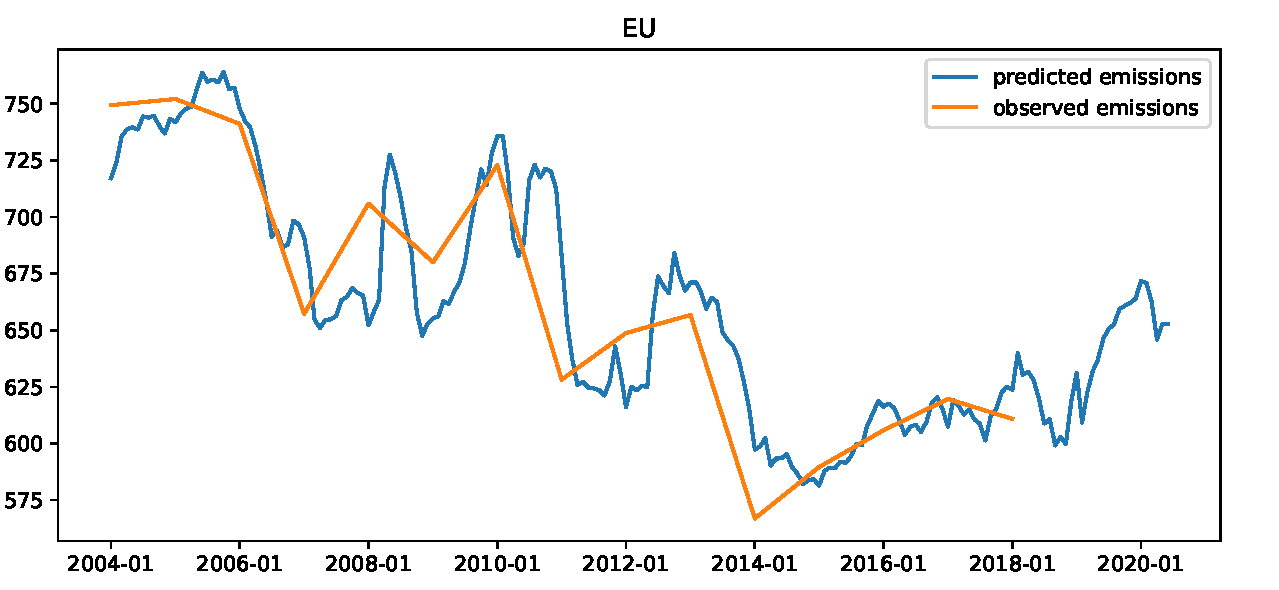
\includegraphics[width=0.5\linewidth]{../buildings/eu}}
	\subfloat[USA]{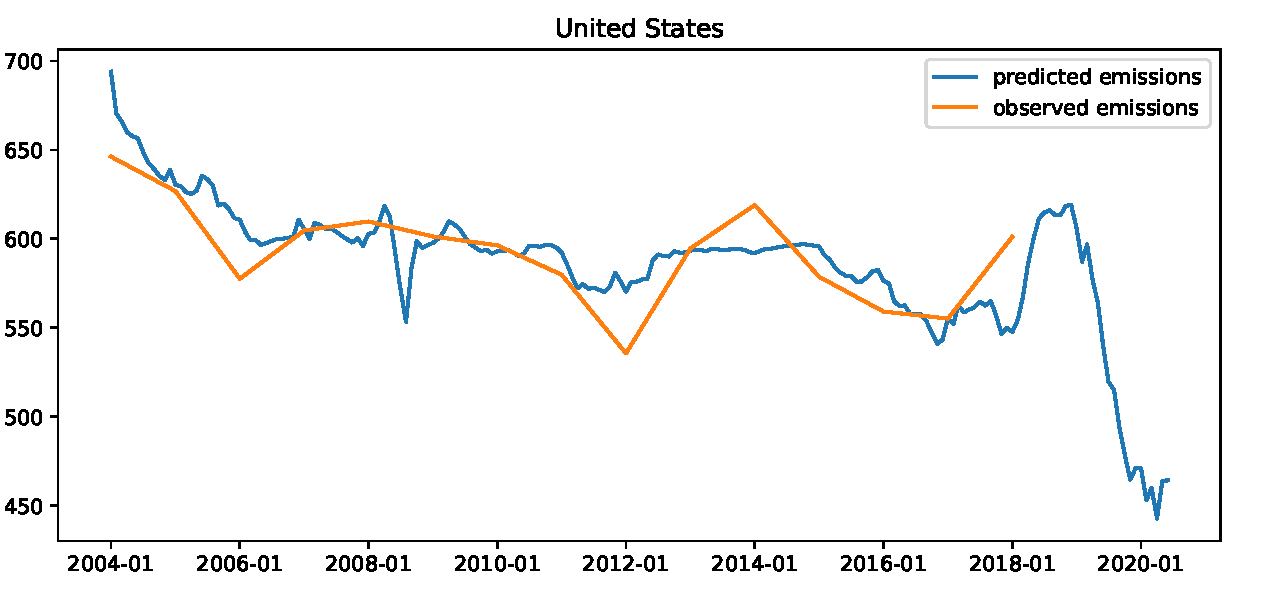
\includegraphics[width=0.5\linewidth]{../buildings/united_states}}\\
	\subfloat[Brazil]{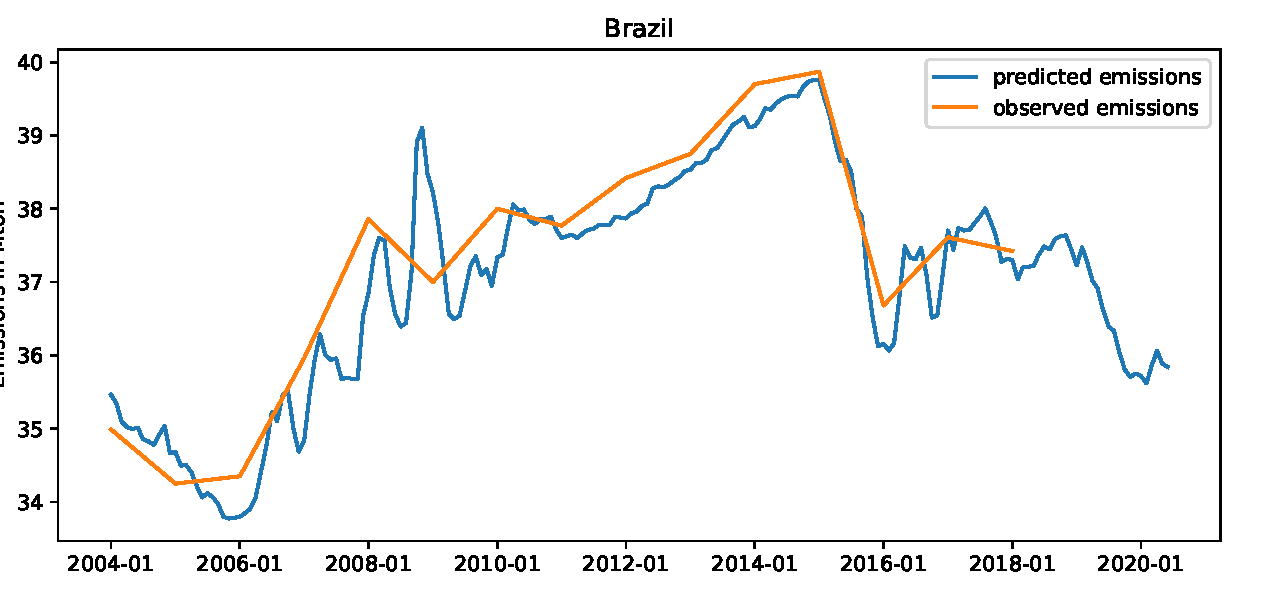
\includegraphics[width=0.5\linewidth]{../buildings/brazil}}
	\subfloat[Russia]{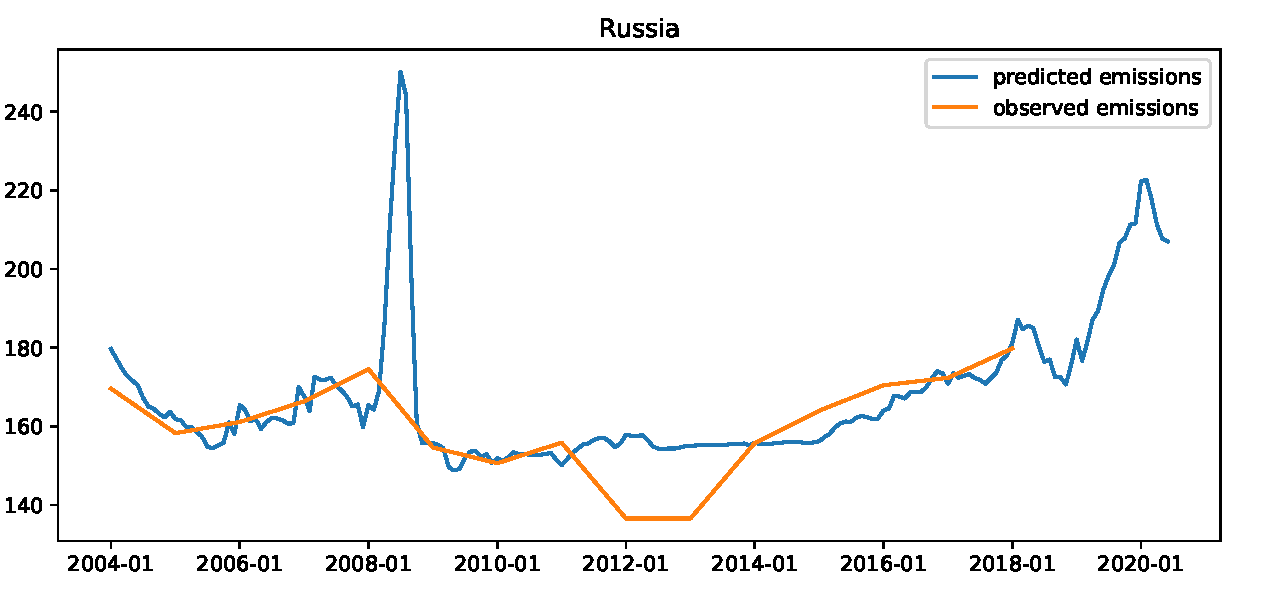
\includegraphics[width=0.5\linewidth]{../buildings/russia}}\\
	\subfloat[India]{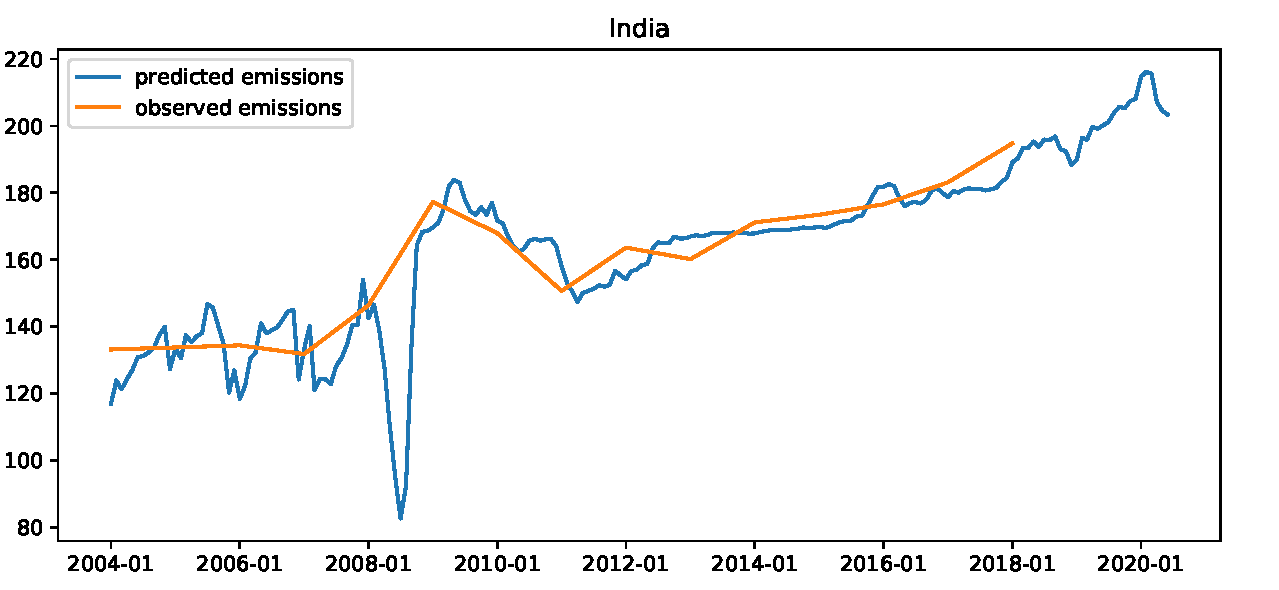
\includegraphics[width=0.5\linewidth]{../buildings/india}}
	\subfloat[Japan]{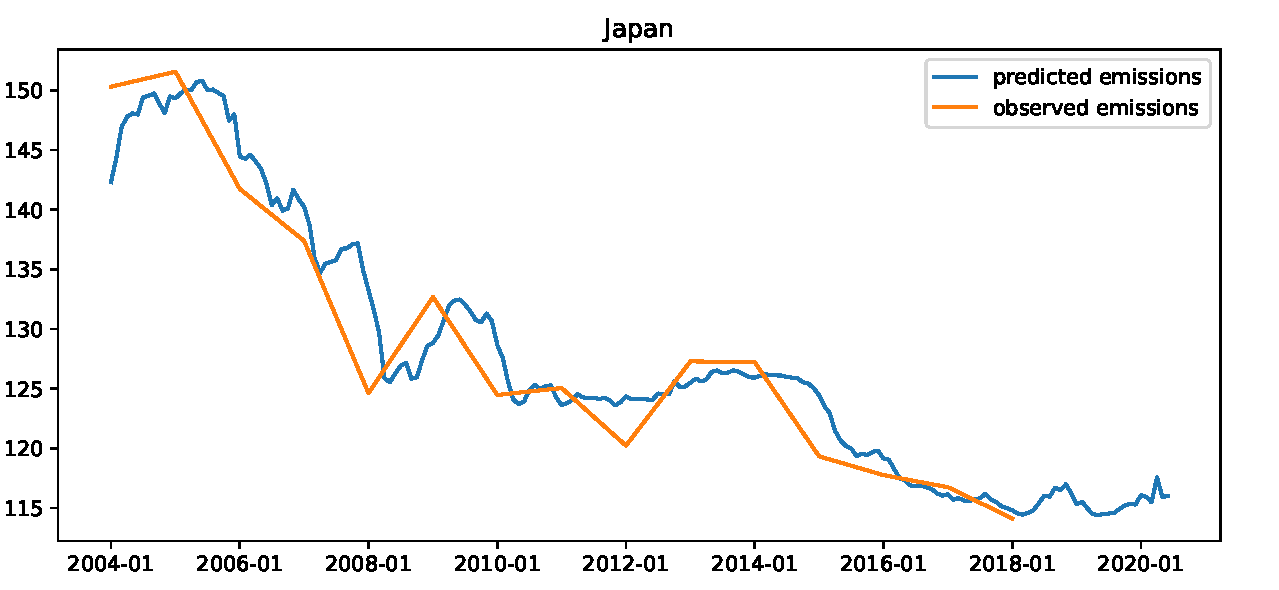
\includegraphics[width=0.5\linewidth]{../buildings/japan}}\\
	\subfloat[Canada]{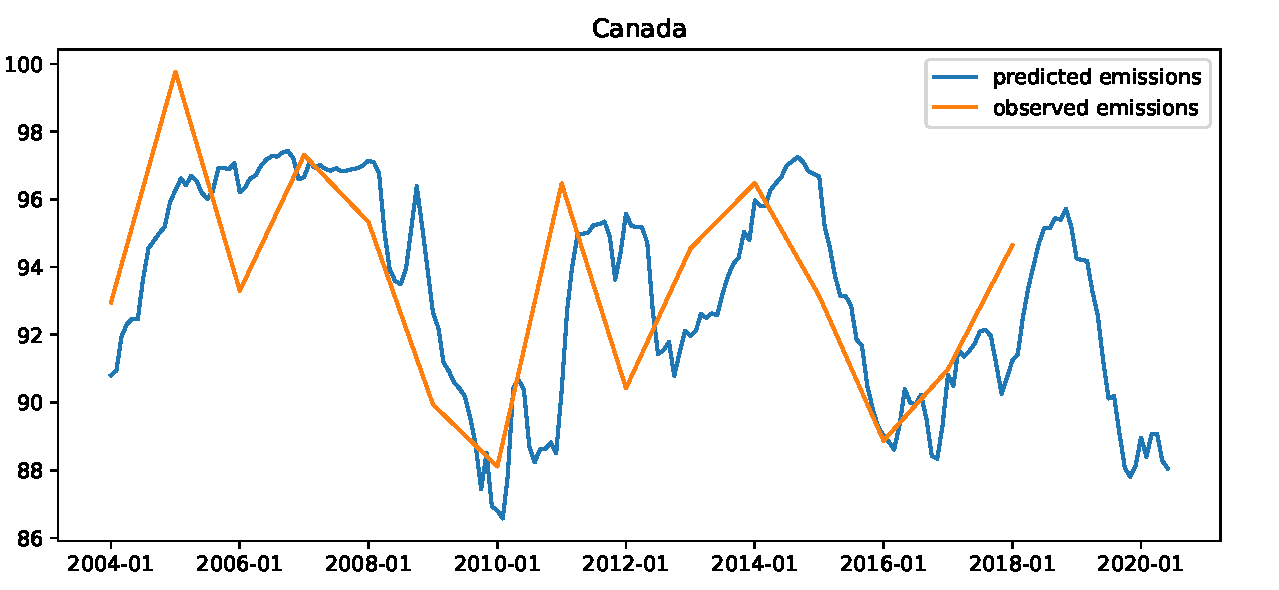
\includegraphics[width=0.5\linewidth]{../buildings/canada}}
	\subfloat[China]{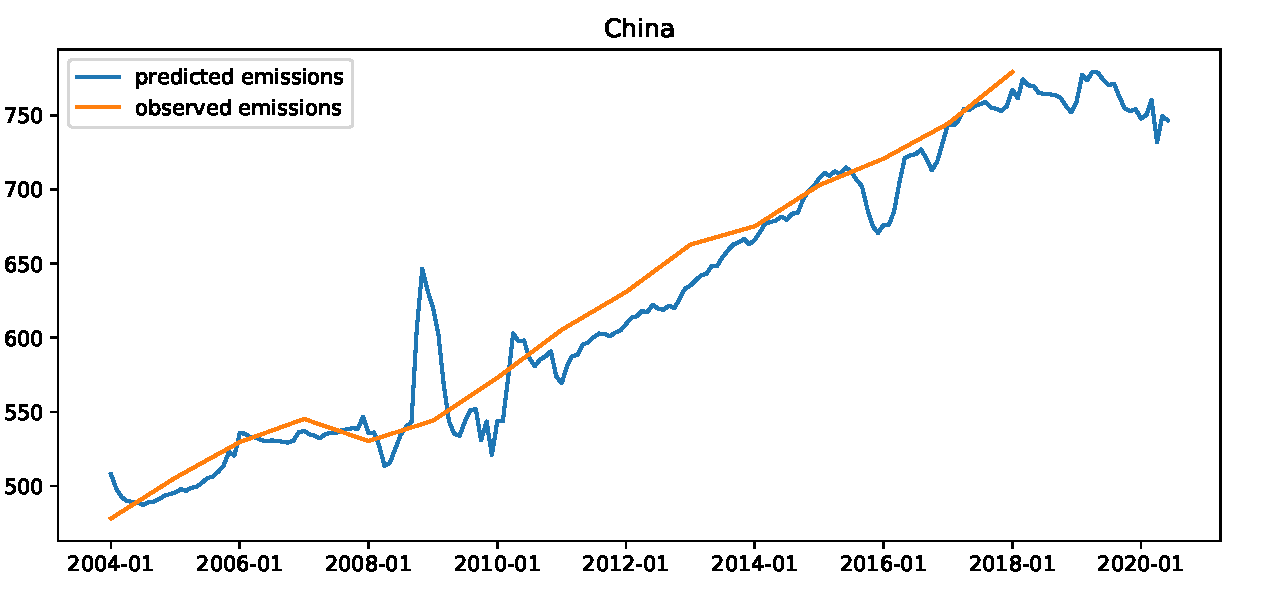
\includegraphics[width=0.5\linewidth]{../buildings/china}}
	\caption{Predicted emissions based on indicators on training set and for 2020.}
	\label{fig:mobility_pred}
\end{figure}	


%Conclusion
\paragraph{Conclusion}

In conclusion, we were able to model the countries sufficiently well. Each country showed an emission drop in the early months of 2020, indicating that COVID-19 had an impact on the indicators and therefore on the overall emissions in the sector.
%todo: scores are lacking
\subsubsection{Mobility data}

\paragraph{Analysis of available datasets}

As already described in Milestone 2, we had four data sets suitable for this sector. These were two data sets on international flight activity and two mobility data sets from Google and Apple. The aviation data sets could not be used for this sector, as the number of flights was not stated explicitly for every country. We then decided to take a closer look at the Apple mobility data set, as it was easy to handle but still contained all necessary information. For every country, it contains \textit{walking} and \textit{driving} mobility data and wherever available, \textit{transit} mobility data as well. We had to pre-process this dataset a little by grouping the data of 26 out of 28 EU countries (Cyprus and Malta were not available). Furthermore, we applied a 7-day \textit{moving average} filter, to account for changes throughout the week. Unfortunately, we could not gather mobility data for China, as it was neither in the Apple mobility data set nor in the Google mobility data set. This can be directly attributed to China's restrictive handling of sensitive data. We also tried to gather information from \textit{Baidu Maps}, China's \textit{Google Maps} equivalent so-to-say. However, this proved to be very difficult, as the files are prepared in Chinese and nobody in our team is able to read Chinese. Therefore, we had to calculate China's mobility indicator from other countries' mobility data and do a few assumptions.

\paragraph{Data visualization}

As it is interesting to see the drop in international flights, we depicted it in \autoref{fig:flights}. In \autoref{fig:driving} and \ref{fig:transit}, we show the raw, unprocessed data and our result after applying a moving average filter. From the two figures, we can see that \textit{driving} mobility almost recovered to a normal level for most countries, while \textit{transit} mobility is still low for all countries except Japan.


\begin{figure}[hb!]
	\centering
	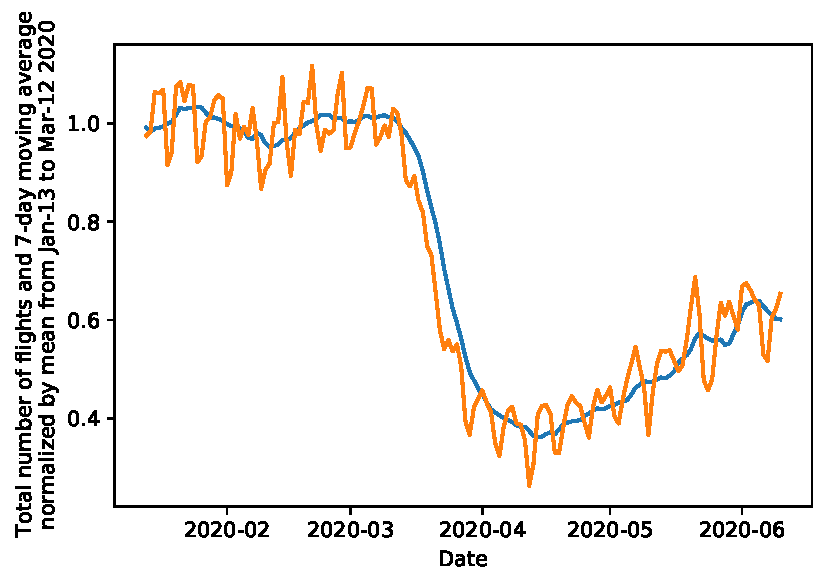
\includegraphics[width=0.7\linewidth]{../predictions/flights.pdf}
	\caption{International flights data.}
	\label{fig:flights}
\end{figure}


\begin{figure}[h!]
	\centering
	\subfloat[Raw driving data]{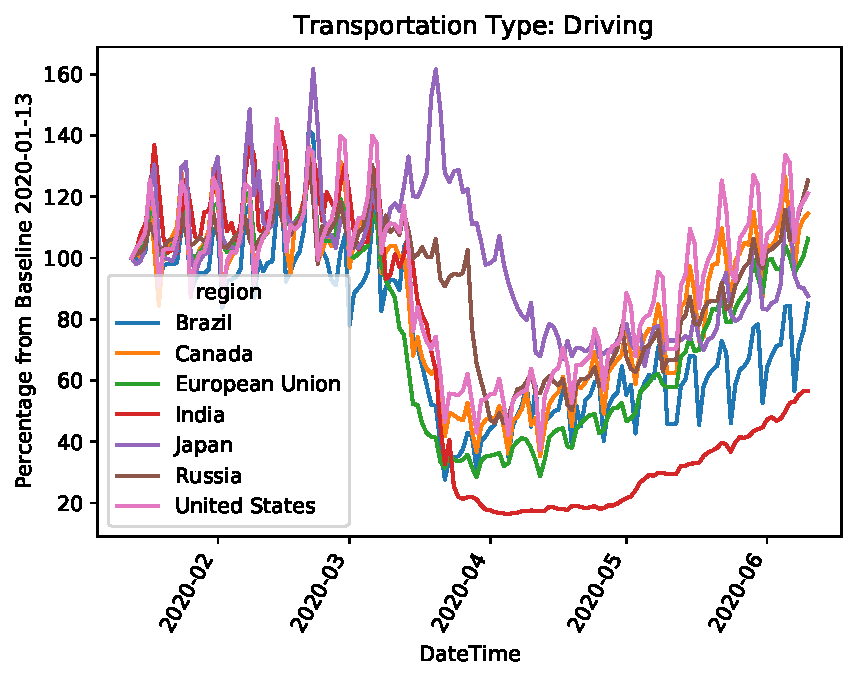
\includegraphics[width=0.48\linewidth]{../predictions/driving.pdf}}
	\hfill
	\subfloat[Driving data with moving average]{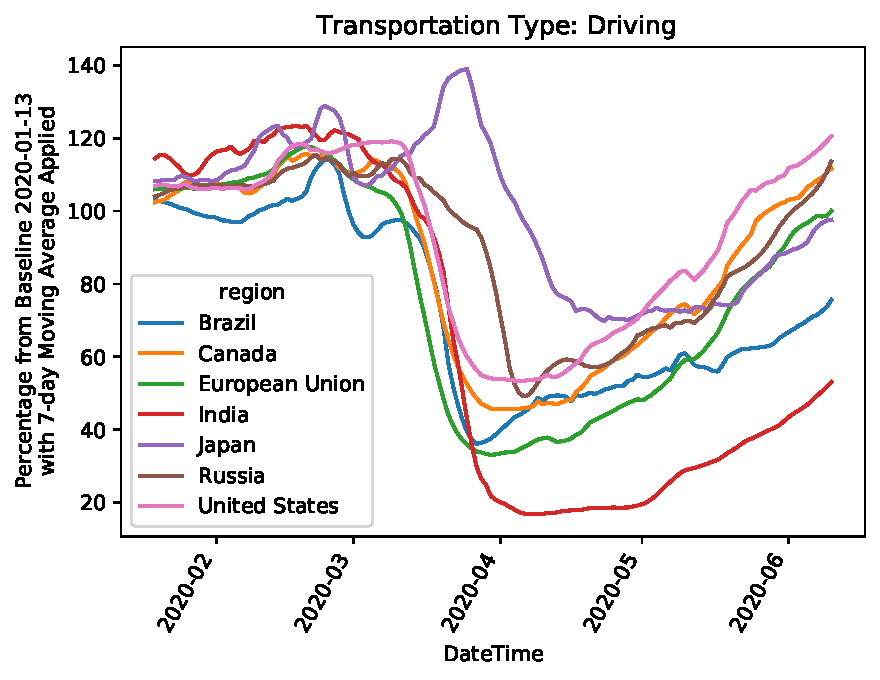
\includegraphics[width=0.48\linewidth]{../predictions/driving_ma.pdf}}
	\caption{Mobility data. A steep drop is visible for all countries.}
	\label{fig:driving}
\end{figure}

\begin{figure}[h!]
	\centering
	\subfloat[Raw transit data]{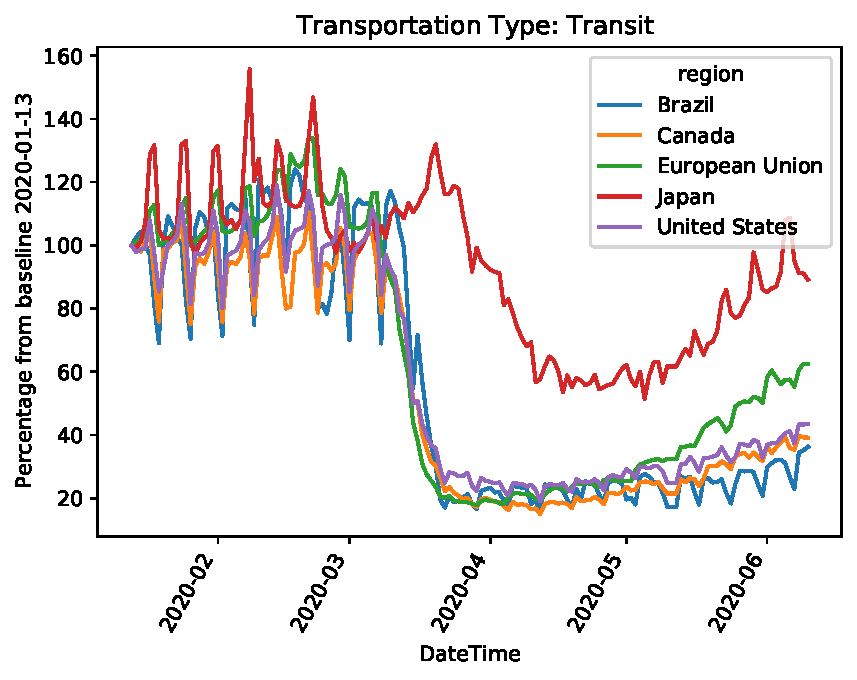
\includegraphics[width=0.48\linewidth]{../predictions/transit.pdf}}
	\hfill
	\subfloat[Transit data with moving average]{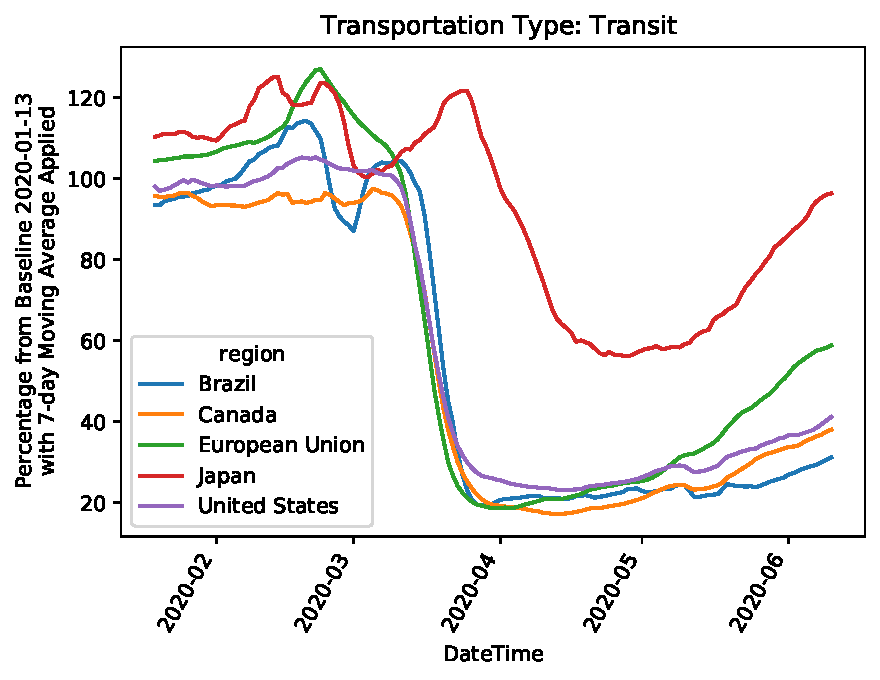
\includegraphics[width=0.48\linewidth]{../predictions/transit_ma.pdf}}
	\caption{Mobility data. A steep drop is visible for all countries that transit data was available for.}
	\label{fig:transit}
\end{figure}

\paragraph{Result}

Due to the huge size of the project, we had to cut back on some details and make some assumptions. As we could not find out the correct contributions of transit and driving mobility to the \co emissions of this sector, we had no choice but to weigh those two categories equally. We then calculated the monthly average, which lead to the resulting indicators depicted in \autoref{fig:indicator_mobility}. As all data is normalized to the first day of available data, all indicators should start at one. But since we are taking the mean of the first month, one can see small deviations from one for most countries.

For China, we had to assume a curve similar to the others and took mean values of suitable countries and set the mobility to one in months were COVID-9 had no to little impact, like January and June.


\begin{figure}[ht!]
	\centering
	\subfloat[Transit indicator]{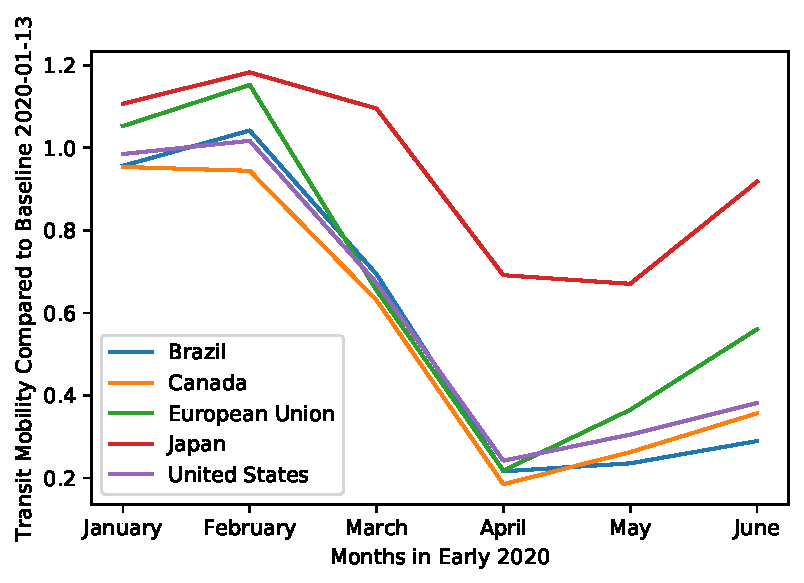
\includegraphics[width=0.48\linewidth]{../predictions/indicator_transit.pdf}}
	\hfill
	\subfloat[Driving indicator]{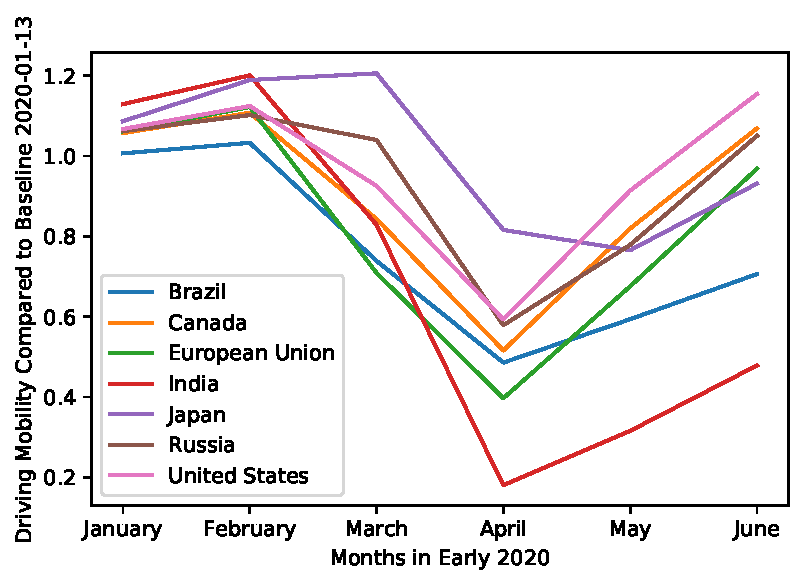
\includegraphics[width=0.48\linewidth]{../predictions/indicator_driving.pdf}}
	\caption{The two \textit{driving} and \textit{transit} mobility indicators before we combine them to one overall mobility indicator.}
	\label{fig:both_mobility_indicators}
\end{figure}

\begin{figure}[hb!]
	\centering
	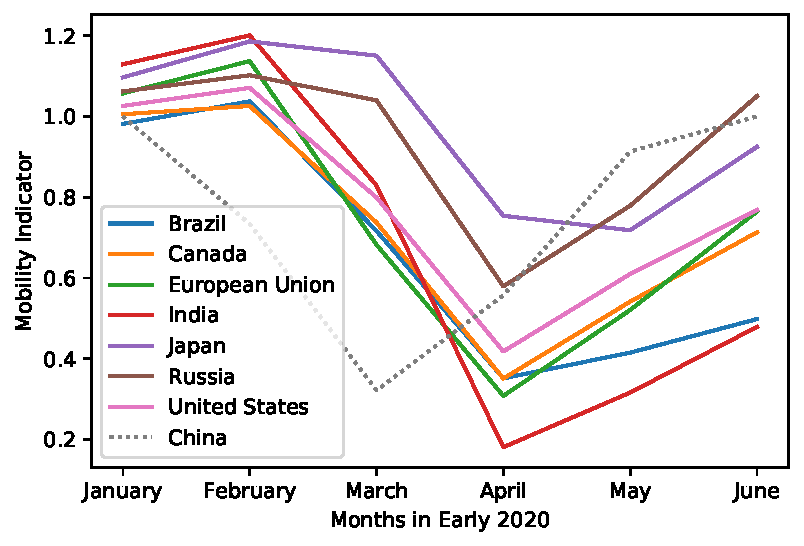
\includegraphics[width=0.7\linewidth]{../predictions/full_mobility_indicator.pdf}
	\caption{Calculated mobility indicator, including China.}
	\label{fig:indicator_mobility}
\end{figure}

\paragraph{Conclusion}

It is very unfortunate that we have no data on China, as it is the biggest emitter of \co. This definitely has an impact on the validity and accuracy of the mobility indicator and therefore the model. Still, we tried to model China's mobility as accurately as possible. As we can see in \autoref{fig:indicator_mobility}, we assume that China's emission drop earlier than the others, which is a fair assumption as the pandemic started in China.
\subsubsection{Other industries}

This sector is called \textit{other industries}, which one might misunderstand at the first glance. We wanted to be consistent with the sector distribution we found, where this sector is labeled other industry. Actually, it simply refers to all industry except \textit{power industry}.

\paragraph{Strategy}
After conducting some research on how to find suitable indicators for this sector, we found out that global steel production fits our needs. Monthly data is readily available and data researchers are able to predict a country's economic growth with it~\cite{Ravazzolo2020}.
Furthermore, \textit{Le Quéré et al.} model monthly \co data of the industry sector using US steel production data as well~\cite{LeQuere2020}.

\paragraph{Data}
We found recent data of worldwide steel production from January 2019 on, depicted in \autoref{fig:steelallcountries}.
For a longer period of time, we found US steel production data. As shown in \autoref{fig:steelUS}, it ranges from mid 2015 until mid 2020.
\begin{figure}[hbt]
	\centering
	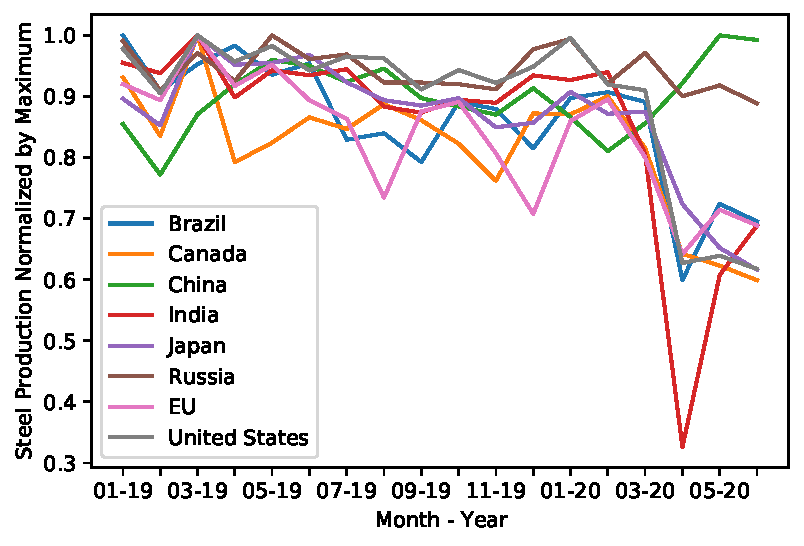
\includegraphics[width=0.69\linewidth]{../predictions/steelAllCountries.pdf}
	\caption{Steel output of all eight countries considered, normalized by the respective maximum for a better comparison.}
	\label{fig:steelallcountries}
\end{figure}

\begin{figure}[hbt]
	\centering
	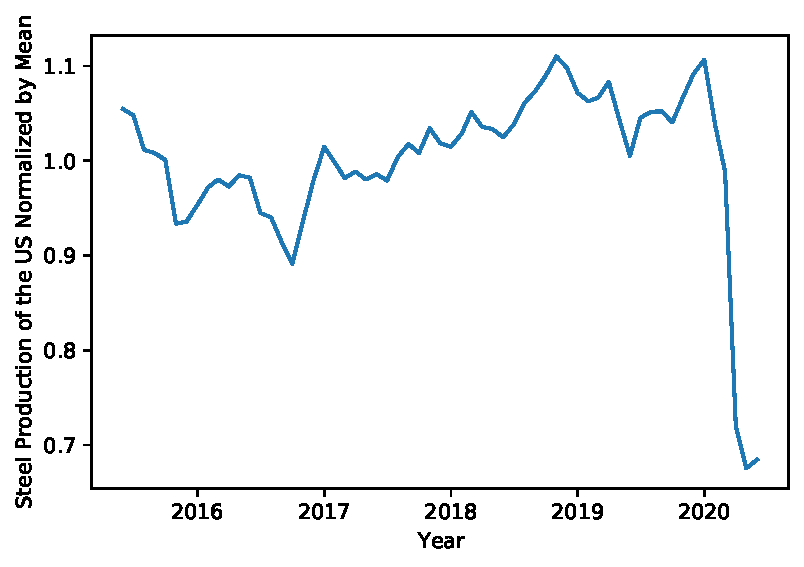
\includegraphics[width=0.69\linewidth]{../predictions/steelUS.pdf}
	\caption{Steel output of the US, normalized by the mean in the years 2015 to 2020.}
	\label{fig:steelUS}
\end{figure}

\newpage

\paragraph{Method}
In contrast to \textit{Le Quéré et al.}, we wanted to use each country's own steel production and not only US data. However, only recent data from 2019 until now is available for free for every country considered in this work. Obviously, one can not find seasonality trends from that. Thus, we use the recent data we have to find a preliminary indicator without seasonality adjustments for each country first, as depicted in \autoref{fig:otherindustry_notadjusted}. For this, we took the early 2020 data of this month and divided it by the early 2020 data and thus obtain a percentage of the steel production output in early 2020 compared to early 2019. 

We then use US steel production data to find a seasonality trend. Furthermore, we assume here that we can transfer this seasonality adjustment to all other countries as well. Our strategy to find a seasonality trend begins with finding mean values of steel production in a given year. We assume that these mean values centered on a given time-point, are the steel production values with seasonality removed. The ratio of the new value without the seasonality effect to the old value is the seasonality trend. Since we can calculate the trend for four different years by using the US data, and we do not want to overfit for a single year, we take the average of seasonality trends of 4 years. Seasonally adjusted steel output of the US can be seen in \autoref{fig:steelUS_adjusted}

\paragraph{Results and conclusion}
As seen in \autoref{tab:otherindustry_seasonality}, our calculated seasonality effect is relatively weak, thus adjusting the data does not have a significant impact. This may also be caused by the limited data.
We can see that for most countries a drop in \co emissions for the \textit{other industries} sector can be expected. For China however, we see more or less stable emissions. This surprised us at first. But the stable steel output can be explained with the fact that COVID-19 only hit a very confined region of China in the beginning and was contained more or less successfully later.

\begin{figure}[hbt]
	\centering
	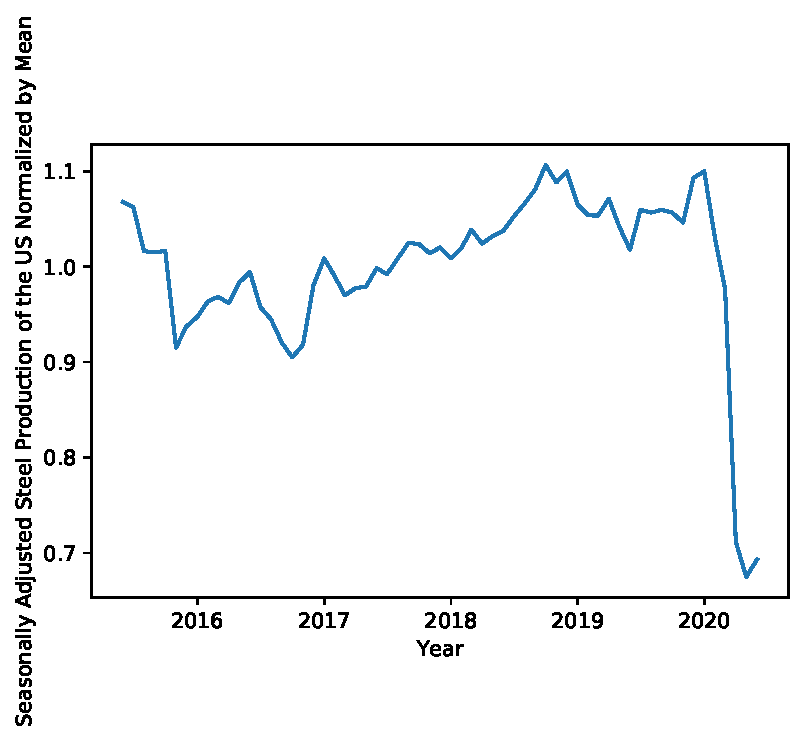
\includegraphics[width=0.69\linewidth]{../predictions/steelUS_seasonadjusted.pdf}
	\caption{Seasonally adjusted steel output of the US, normalized by the mean in the years 2015 to 2020.}
	\label{fig:steelUS_adjusted}
\end{figure}


\begin{table}[h!]
	\centering
	\begin{tabular}{cccccccccccc}
		\hline
		January & February & March & April & May & June & July & August & September & October & November & December\\
		\hline
		\hline
		0.995 & 0.993 & 0.989 & 0.99 & 1.0 & 1.014 & 1.015 & 1.006 & 1.008 & 1.017 & 0.982 & 1.003\\
		\hline &&&&&&&&&&& \\
	\end{tabular}
	\caption{Seasonality trend of steel production in the US.}%todo: source
	\label{tab:otherindustry_seasonality}
\end{table}

\begin{figure}[h]
	\centering
	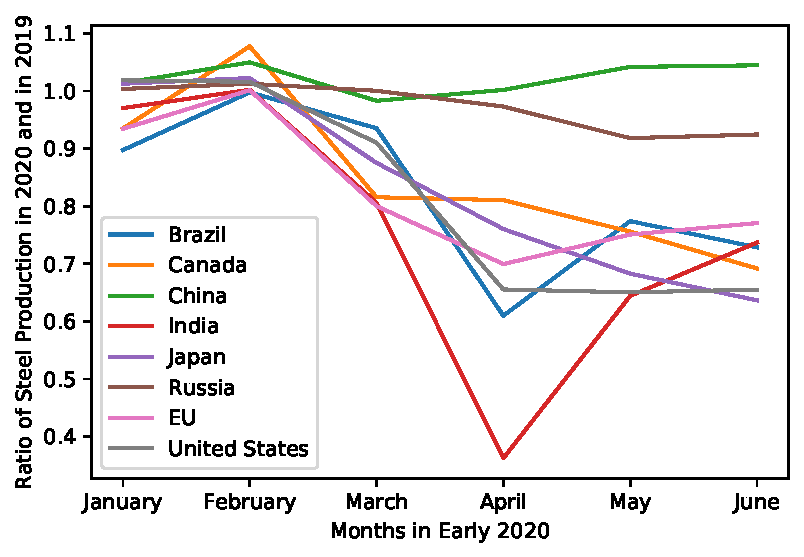
\includegraphics[width=0.7\linewidth]{../predictions/otherindustries_notadjusted.pdf}
	\caption{The indicator of each country without seasonality adjustments.}
	\label{fig:otherindustry_notadjusted}
\end{figure}

\subsubsection{Other sectors}

The main sector which has a big impact on the \co emission considered such as \emph{other sectors} is agriculture. In 2018, it had an average contribution of 12.56\% to the worlds greenhouse gas emissions. In this section, we considered agriculture indicators which can have the most impact on the \co emission, such as rice and soybeans cultivation, and cattle farming. 

\paragraph{Indicators}

\subparagraph{Cattle farming}

Without any doubts, we can say that it is the livestock farming which has the greatest impact on \co emission in this sector. Cattle farming has a huge impact on the greenhouse gas emissions not only by breathing. The carbon balance of livestock farming includes emissions related to land-use changes, in particular the replacement of forests with pastures and arable fields for fodder production (i.e. deforestation). This means the elimination of huge carbon reservoirs, which are forests, and their replacement with much less capacious agricultural areas. It is estimated that as a result of deforestation, up to 2.4 billion tons of \co are emitted into the atmosphere per year. It is the largest item in the balance of not only \co emissions from animal farming, but also the total greenhouse gas emissions from agriculture sector.

We takes into account 8 selected regions (USA, EU, Brazil, Russia, Japan, China, India and Canada), where 4 of them are the biggest world's providers of cattle (Brazil, India, USA, China) to show the trends in the recent 7 years and compare it with the estimation for all 2020 year. Because the recent data is very hard to collect, we are not able to say how fulfilled is this estimation for now. 

\begin{figure}[hb]
	\centering
	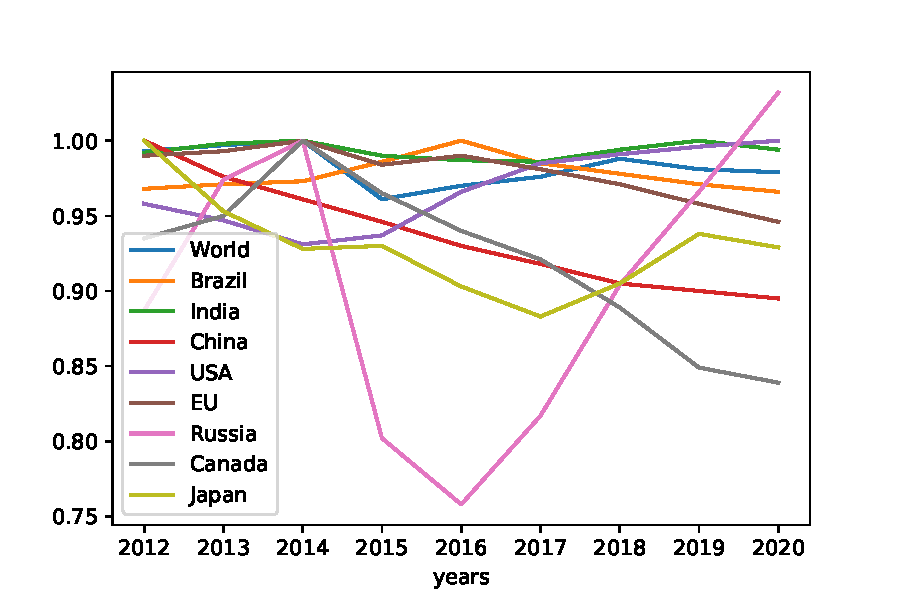
\includegraphics[width=0.7\linewidth]{../agriculture/Graph_cattle.pdf}
	\caption{Trends of cattle agriculture for 8 selected areas in seasons 2012-2019 with the estimation for all season 2020}
	\label{fig:Graph_cattle}
\end{figure}


\subparagraph{Plants: Analyzing rice and soybeans as indicators}

The greenhouse gas emissions profile for plant production differs significantly from that for sectors such as transport or industry. Emissions come from naturally variable biological processes that are numerous and complex, and management of these unavoidable emissions from biological processes is limited. Plant production naturally traps carbon in the soil and biomass during soil processes, also plants absorb \co from the atmosphere by photosynthesis. The emission results from the use of organic and inorganic fertilizers in the soil, as well as from the activity of microorganisms in the process of denitrification and nitrification. The potential to reduce the emissions of greenhouse gases from plant production gives the opportunity to combat global warming. 

We selected two plants which can have the biggest impact on greenhouse gas emission, soybean and rice. In case of rice, Canada is the most northerly rice production country and it has only one hectare crop of rice. That is why we decided to reject this country in our consideration in this sector. 

\begin{figure}
	\centering
	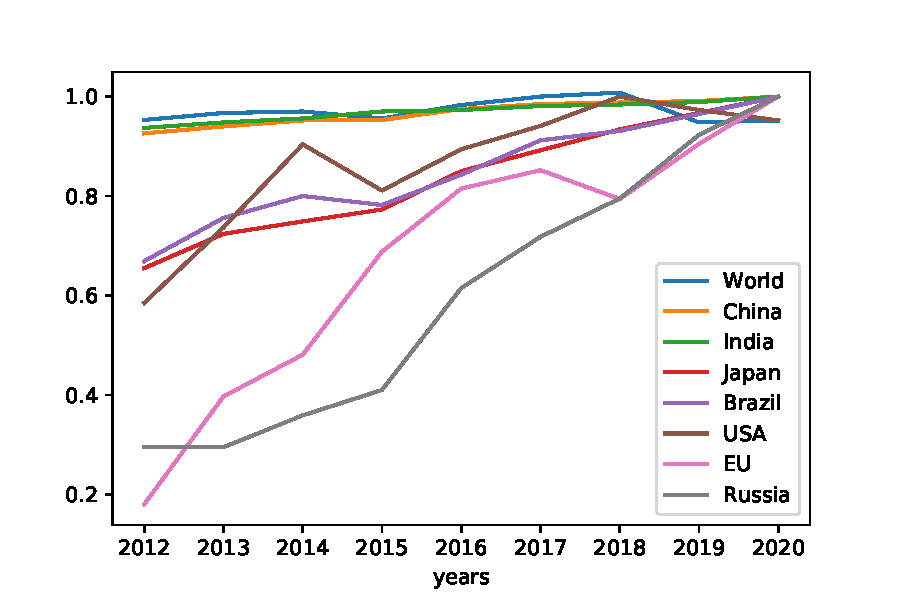
\includegraphics[width=0.7\linewidth]{../agriculture/Graph_rice.pdf}
	\caption{Trends of rice agriculture for 8 selected areas in seasons 2012-2019 with the estimation for all season 2020}
	\label{fig:Graph_rice}
\end{figure}

\begin{figure}
	\centering
	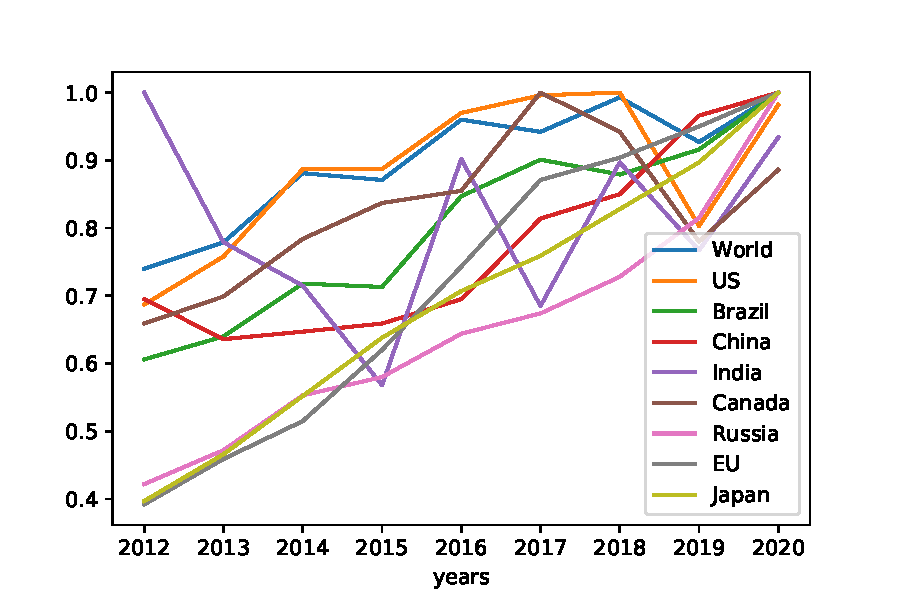
\includegraphics[width=0.7\linewidth]{../agriculture/Graph_soybean.pdf}
	\caption{Trends of soybean agriculture for 8 selected areas in seasons 2012-2019 with the estimation for all season 2020}
	\label{fig:Graph_soybean}
\end{figure}

We tried to gather detailed data on the processes that affect greenhouse gas emission from rice agriculture and their inter-relationships. It defines the shifting roles and potential future of these gases in causing global warming and the benefits and trade-offs of reducing emissions. It is known that when large amounts of organic matter are applied, the additional flux that is observed is due to both greater production and reduced emission. We noticed that rice cultivation is becoming less environmentally friendly in the face of a changing atmosphere. This is important because rice fields are one of the largest sources of methane and rice is the second most cultivated crop. Considering this issue with our project is to relate the \co emission and try to say how rising temperatures and the extra amount of carbon dioxide in the atmosphere affect rice crops and the amount of methane (CH\textsubscript{4}) released. It was figured out that the greater presence of \co resulted in increased methane emissions from rice fields, and in addition, high temperatures caused crops to decline. The methane in the rice fields is produced by microorganisms that absorb carbon dioxide. The more \co, the faster the rice grows, and the accelerated plant growth gives the microorganisms more energy. Rising \co levels will increase rice yields, but also the amount of methane. As a result, the amount of CH\textsubscript{4} emitted per kg of rice will increase. Rising temperatures have little effect on methane emissions, but as they reduce yields, the average amount of methane per kg of rice will increase. As a result, the higher \co concentration and higher temperatures projected at the end of the century may double the amount of methane per kg of rice produced. There are several options for reducing the amount of CH\textsubscript{4}, such as using alternative fertilizers and growing varieties that are less sensitive to heat.

Seeing that rice agriculture can have huge impact on the greenhouse gases emission, we try to show if there is any impact of COVID-19 pandemic on the rice production in the first half of the year, according to the estimation for the year 2020 and the seasonality of growing this crop. In the North China plains, the rice season is from May/June to August/September. In the Yangtze River Valley, rice is planted from April to June and harvested from August to October. In south-eastern China, the early (March to July) and late (June to November) rice crops are bountiful. So we can simplify that in all China there are two main seasons in the first half of the year and in the second half of the year. Taking India into account, the main rice growing season is June-July and it is harvested in November-December. The third world largest rice provider is Japan. In central Japan, it is from April–May to August–October. In southern Japan the rice season is from April -May to August–September. In Brazil the rice is planted from September to December and harvested from February through June, although later-planted rice grown in the northeast extends the season to August. In United States the harvest season in mid-September to October. 

\vfill

\begin{table}[h!]
	\centering
	\begin{tabular}{c c} 
 	\hline
 	Country & Season\\ 
	 \hline\hline
	 China & March to July and June to November \\ 
	 India & November to December  \\
	 Japan & April-May to August-October \\
	 Brazil & February to June \\
	 USA &  mid-September to October \\ 
	 \hline
	 &\\
	\end{tabular}
	 \caption{Simplification of main seasonality periods of rice harvesting for 5 selected areas.}
	 \label{tab:Seasonality_rice}
\end{table}

Next, we consider another one of a second biggest agriculture crop, soybean. The increase in soybean production as a source of protein and oil is being stimulated by the growing demand for livestock feed, food and numerous other applications. Significant greenhouse gas emissions can result from land use change due to the expansion and cultivation of soybean. However, this is complex to assess and the results can vary widely. The main point shows the importance of land use change in soybean greenhouse emissions, but significant differences were observed for the alternative scenarios, namely 0.1-17.8 kg \co per 1kg of soybean. The original land choice is a critical issue in ensuring the lowest soybean greenhouse balance and degraded grassland should preferably be used for soybean cultivation. The highest emissions occurs for tropical moist regions when rain forest is converted into soybean plantations. When land use change is not considered, the greenhouse gas emission intensity varies from 0.3 to 0.6 kg \co per 1 kg of soybean. It was calculated that all systems in tropical regions have higher greenhouse gas emissions than the others. It is also known, that N\textsubscript{2}O emissions play a major role in the greenhouse gas emissions from cultivation, although N\textsubscript{2}O emission calculations are very sensitive to the parameters and emission factors adopted.
If it comes to seasonality of soybean agriculture, the most of world soybean is harvested between March and the end of July (even in Brazil). In some tropical regions it can occur also during the winter season from November to December, but the amount does not have big impact for the world's production.

\subparagraph{Results}

\begin{table}[h!]
	\centering
	\begin{tabular}{c c c c} 
		\hline
		Country & Estimation for 2020 season & State for 1st June 2020 & Percent \\ 
		\hline\hline
		World & 470.98 & 394.43 & 83.74\% \\
		China & 150.43 & 110.32 & 73.33\% \\ 
		India & 119.43 & 15.76 & 13.19\% \\
		Japan & 7.98 & 5.34 & 66.92\% \\
		Brazil & 7.65 & 7.82 & 102.2\% \\
		USA & 6.76 & 1.32 & 19.53\%  \\ 
		EU & 1.89 & 1.87 & 98.94\% \\
		Russia & 0.78 & 0.82 & 105.13\% \\
		\hline
		&&& \\
	\end{tabular}
	\caption{The current state of rice crops for the World production and 7 selected areas with a comparison to the estimation for the all 2020 season}
	\label{tab:Current_production_rice}
\end{table}

Analyzing \autoref{tab:Current_production_rice} with current data and seasonality of the rice agriculture, we can simply say that there is no impact on this sector during the COVID-19 pandemic. In some countries current state is even higher than the estimated one, whereas in countries where it's lower it basically depends on the seasonality in the particular region. 

 

\begin{table}[h!]
	\centering
	\begin{tabular}{c c c c} 
 	\hline
 	Country & Estimation for 2020 season & State for 1st June 2020 & Percent \\ 
	 \hline\hline
	 World & 362.76 & 345.12 & 95.14\% \\
	 US & 118.32 & 112.26 & 94.88\% \\ 
	 Brazil & 135.40 & 131.0 & 96.75\% \\
	 China & 18.78 & 17.5 & 93.18\% \\
	 India & 11.39 & 10.5 & 92.19\% \\
	 Canada & 6.84 & 6.15 & 89.91\%  \\ 
	 Russia & 5.19 & 4.72 & 90.94\% \\
	 EU & 3.42 & 2.61 & 76.32\% \\
	 Japan & 0.58 & 0.34 & 58.62\% \\
	 \hline
	 &&& \\
	\end{tabular}
	 \caption{The current state of rice crops for the World production and 8 selected areas with a comparison to the estimation for the all 2020 season}
	 \label{tab:Current_production_soybean}
\end{table}

Analyzing \autoref{tab:Current_production_soybean} with current data and seasonality of the soybean agriculture, we can say again, without any doubts that there is no impact on this sector. In countries where it is lower it strongly depends on the seasonality period which occurs till the end of July, and the final state can be even higher that the estimated one. 

\paragraph{Conclusion}

In conclusion, whereas both, the livestock and the plant growing has an impact on the \co emission, we can easily notice that COVID-19 does not have impact on the agriculture. Of course there can be some differences between estimated values and the current data because of many factors associated with the global pandemic and lock down, but it has minimal impact in general overview. 
However, there are other concerns related to the pandemic and agriculture. Farmers are afraid that COVID-19 can have an impact not on the production size, but production distribution, and this distribution can contribute to some problems for countries that are dependent on imported crops and for farmers who can't sell their yields. Nonetheless this phenomenon is not a part for our consideration. 

%%%%%%%%%%%%%%%%%%%%%%%%%

\subsection{COVID-19 Data}
\paragraph{Calculating the severity of COVID-19}

Since the purpose of this project is to investigate the correlation between COVID-19 pandemic and  $CO_2$ emissions, we needed a dataset, that provides recent and detailed information on COVID-19 statistics per country. These necessary statistics include number of cases, deaths and recoveries. Accessibility, detail and up-to-dateness of Bing COVID-19 dataset \cite{Bing} made it our primary choice for getting COVID statistics.

Eventually we will need to compare the change in $CO_2$ emissions against the severity of COVID-19 cases in a given country. Since the values in Bing database are absolute, we also need population data for each country. After we combined population information, extracted from \cite{PopulationData}, with COVID-19 statistics, we were able to calculate the severity of COVID-19 in any given country, i.e. deaths and cases per 100,000 people. These rates are visualized in \autoref{fig:covidimpact}. This information is to be compared and correlated with predicted $CO_2$ emissions.

\begin{figure}[h]
	\centering
	\begin{subfigure}[b]{0.47\linewidth}
		\includegraphics[width=\linewidth]{../covid/case rate}
	\end{subfigure}
	\begin{subfigure}[b]{0.47\linewidth}
		\includegraphics[width=\linewidth]{../covid/death rate}
	\end{subfigure}
	\caption{Covid-19 rates for each country.}
	\label{fig:covidimpact}
\end{figure}


\begin{figure}[h]
	\centering
	\begin{subfigure}[b]{0.47\linewidth}
		\includegraphics[width=\linewidth]{../covid/bing_top5}
	\end{subfigure}
	\caption{5 countries which have the highest number of cases.}
	\label{fig:bingtop5}
\end{figure}
%\subsection{Analysis of climate agreement goal fulfillment dependence on COVID-19 severity}

\begin{figure}
	\centering
	\includegraphics[width=0.7\linewidth]{../DataPipelineResults/reduction_co2_vs_country_goal_rate}
	\caption{}
	\label{fig:reductionco2vscountrygoalrate}
\end{figure}

%%%%%%%%%%%%%%%%%%%%%%%%%%%%

\section{Results and Discussion}

%How complete is our model so far? What can we model? How big are the uncertainties?
%
%What where the models and approaches that performed the best? \dots for each sector:
%Which sectors were most important (biggest fraction of emissions)

With indicators for all sectors, we can now model how the \co emissions for each of the eight countries behaved for the first half of 2020. For that, we combine all sectors for each country according to each sector's contribution.


We provide our result in \autoref{fig:predictedCO2}. The data is seasonality adjusted already, which means that the height of each line directly gives the fraction of \co emissions we would have expected for this month. This is our main result for this Milestone and it completely meets our expectations. We took a lot of different data into account and tried to model \co emissions as accurately as possible with our (limited) resources. Since we took so many different data sets into consideration we think it is fair to assume that we minimized the overall uncertainty. We used a lot of different machine learning models, each one carefully chosen such that we obtain the best results only. 

We still think that we could have done even better with more resources but nevertheless, we are very satisfied with the outcomes of our model so far. We therefore conclude that our model and approach is valid, delivering a result with which we can finally compare COVID-19 case numbers now. This will be done in the next and final Milestone.

\begin{figure}[hb!]
	\centering
	\includegraphics[width=0.7\linewidth]{../predictions/change_rate.pdf}
	\caption{Change of CO2 emissions for each country we consider. As expected, we observe a drop in \co emissions.}
	\label{fig:predictedCO2}
\end{figure}


%\begin{itemize}
%	\item \textbf{Transport:}
%	\item \textbf{International Aviation/Shipping:}
%	\item \textbf{Buildings:}
%	\item \textbf{Other industrial combustion:}
%	\item \textbf{Other sectors:}
%	\item \textbf{Power industry:}
%\end{itemize}
\section{Front-End Mock Up}

In the previous milestones we already created a frond-end in order to provide an interactive visualization of our collected datasets. This front-end was built using python dash, a framework that builds on top of Flask and React. The respective webserver is deployed by use of Heroku and can be found at the following URL: \url{https://ami-group1-dashboard.herokuapp.com/}.

In order to present our final results, the same framework will be used. In particular, the website will be divided into multiple sections. Our goal is to use the front-end in order to show what datasets were used, how the model pipeline is structured and of course to show the final conclusion in regard to the research question. The basic layout is shown in Figure \ref{fig:front_end_title_page}.

\begin{figure}[h!]
\centering
\includegraphics[width=0.9\textwidth]{front_end_title_page}
\caption{Frontend title page}
\label{fig:front_end_title_page}
\end{figure}

As shown above, the different sections are divided into COVID-19 data, greenhouse gas data and indicators for various industries. In order to get an intuition about what our model pipeline looks like, there will be a separate section which graphically describes the entire pipeline. A preliminary version for this can be seen in Figure \ref{fig:model_pipeline}.

\begin{figure}[h!]
\centering
\includegraphics[width=0.9\textwidth]{mock-up_frontend_pipeline_description.pdf}
\caption{Model pipeline description}
\label{fig:model_pipeline}
\end{figure}

Finally, there will be a section showing our final results. In order to show the training-process, one possibility would be to let the model train while highlighting parts in the diagram shown above which are currently trained. This would be the most descriptive way we could provide our model pipeline to the reader. But since we use quite a variety of different models and some training steps require a lot of computational effort, this approach might not be feasible with regard to costs of the web instances we use, in this case provided by Heroku. This issue could be adressed by just partially training the model parts which are not that compuationally expensive.

On the other hand, there will not be significant advantages using a live-training approach compared to directly showing the results of pre-trained models. This is compuationally affordable for us and still can be done in an attractive way. Besides, the reader does not have to wait in order to get the results presented.

Those are the reasons why from the current point of view, we will not include live-training into our website. Still, we will try to keep it as interactive as possible. In particular, the reader should have the ability to select from different countries, inspect their CO2 emissions, the pandemic development and analyse the overall impact of COVID-19 on greenhouse gas emissions. Apart from that, we are planning to integrate some variability for the reader to hypothetically modify the impact of COVID-19. For example, one could then explore how the emissions would have behaved if COVID-19 had even more affected our daily lives in the first half of the year 2020. Another option could also be to explore how a second wave of COVID-19 in some specific countries, similar to the first one, could affect greenhouse gas emissions in the future.

Those interactive options, together with the final result of our research, will be shown on a last tab on the website (currently not available). Here we will present, for the biggest greenhouse gas emitting countries, the impact of COVID-19 on emissions which eventually will be compared to goals stated in the Paris Climate Agreement.

%Add a pointer to heroku page, add prediction plots and extracted information
\section{Dead Ends}

Some approaches we had to give up, as they did not work out well or went in the wrong direction. Still, a short summary of what we did shall be given here.

\subsection{SARIMA model for global CO\textsubscript{2} levels}

We put a lot of effort in predicting global \co levels, until we noticed that this would not help us directly. We thought that we could see a drop in \co levels but this is actually not the case. Even with the emissions going down, levels still rise. The forecast itself is still pretty good we think, it perfectly follows the seasonality of actual \co levels. Our work was not for nothing though, as we could apply our knowledge on SARIMA models later to forecast indicators.

%\begin{figure}[h!]
%	\centering
%	\subfloat[Raw driving data]{\includegraphics[width=0.4\linewidth]{../sarima_co2/allCO2data.pdf}}
%	\hspace{1cm}
%	\subfloat[Driving data with moving average]{\includegraphics[width=0.4\linewidth]{../sarima_co2/dyn_pred_forecast.pdf}}
%	\caption{Mobility data. A steep drop is visible for all countries.}
%	\label{fig:driving}
%\end{figure}

\begin{figure}[hb!]
	\centering
	\includegraphics[width=0.7\linewidth]{../sarima_co2/dyn_pred_forecast.pdf}
	\caption{\co levels from 2015 until beginning of 2020 in blue and a forecast to mid 2021 in orange, including an area of uncertainty in gray.}
	\label{fig:flights}
\end{figure}

\subsection{Weather data}

We also tried to gather satellite precipitation data for the whole world and even had correspondence to data scientists at NASA to explain to us how to access the data. However, when we turned away from our first approach by going with \co levels, we also did not need weather data anymore. Precipitation mainly affects \co levels, not \co emissions. Therefore, this also became a dead end.

\subsection{Recursive Neural Network for predicting athmospheric \co concentration in the future}

One of our first attempts was to predict atmospheric \co emissions in the future by use of pure time series \co concentration data.  Since a mostly generic RNN architecture would serve as a basic structure for other time series predictions as well, we implemented a RNN that could be used for several problems. Only predicting one outcome per cycle and recursively using this result for predicting multiple time steps was not successful at all, even after some optimization steps. An example for one of those results can be seen in the following Figure \ref{fig:RNN1}. In this particular case, a RNN with a single hidden layer with 500 neurons and ten steps as inputs was used.

\begin{figure}[hb!]
	\centering
	\includegraphics[width=0.7\linewidth]{./RNN_athmospheric _CO2_prediction/500neurons_10_inputs_1_output.jpg}
	\caption{\co First attempt: predicting a single output recursively.}
	\label{fig:RNN1}
\end{figure}

Alternatively, predicting multiple time steps in one single cycle was much more successful. Still, the results which are shown in Figure \ref{fig:RNN2} were not convincing at all. In this case, 1000 neurons within the single hidden layer with five inputs were used. In one step, 100 outputs were predicted.

\begin{figure}[hb!]
	\centering
	\includegraphics[width=0.7\linewidth]{./RNN_athmospheric _CO2_prediction/1000neurons_5inputs_100_outputs.jpg}
	\caption{\co Predicting multiple steps in the future.}
	\label{fig:RNN2}
\end{figure}

After taking into account knowlegde we gained from the lecture, the reading assignments and discussing the occured issues, we decided to split the time series data into a trend and a seasonal component. The implemented RNN served for predicting the seasonal behavior in the future. This much more convincing result can be seen in Figure \ref{fig:RNN3}. For predicting the trend component, a simple multi layer perceptron was used.

\begin{figure}[hb!]
	\centering
	\includegraphics[width=0.7\linewidth]{./RNN_athmospheric _CO2_prediction/seasonal_predictions}
	\caption{\co Predicting only seasonal behavior.}
	\label{fig:RNN3}
\end{figure}


\section{Conclusion and Outlook}

As already discussed in the respective sections, we had to come up with several assumptions throughout our project so far. Some of these assumptions can be considered fair, with some we are not really happy. Given the circumstances, we tried to be as precise and accurate as possible, taking all kinds of possibilities into account. Overall, we are confident that we predicted plausible values for the \co emissions of each country we consider for our project. Our data analysis pipeline is therefore set up and we did most of the work for our project in this Milestone. 

All that is left for the next Milestone now is to compare our results and see if \co emissions correlate with COVID-19 data. Also, we will need to finalize our front-end, which should not be too much work given the current status of it. Since a live-training process on the front-end is not valuable for our project, we want to provide interactivity by offering the possibility of hypothetically changing real world scenarios to explore the impact of different pandemic developments. Of course, we will do the final video to explain our whole model in one go. This is definitely an important and integral part of our project, as it is indeed a huge project.

\bibliographystyle{unsrt}
\bibliography{references}  %%% Remove comment to use the external .bib file (using bibtex).
%%% and comment out the ``thebibliography'' section.


%%% Comment out this section when you \bibliography{references} is enabled.



\end{document}
